	%%  A simple AAU report template.

%  2014-09-13 v. 1.1.0
%  Copyright 2010-2014 by Jesper Kjær Nielsen <jkn@es.aau.dk>
%
%  This is free software: you can redistribute it and/or modify
%  it under the terms of the GNU General Public License as published by
	%  the Free Software Foundation, either version 3 of the License, or
%  (at your option) any later version.
%
%  This is distributed in the hope that it will be useful,
%  but WITHOUT ANY WARRANTY; without even the implied warranty of
%  MERCHANTABILITY or FITNESS FOR A PARTICULAR PURPOSE.  See the
%  GNU General Public License for more details.
%
%  You can find the GNU General Public License at <http://www.gnu.org/licenses/>.
%
%  A simple AAU report template.
%  2014-09-13 v. 1.1.0
%  Copyright 2010-2014 by Jesper Kjær Nielsen <jkn@es.aau.dk>
%
%  This is free software: you can redistribute it and/or modify
%  it under the terms of the GNU General Public License as published by
%  the Free Software Foundation, either version 3 of the License, or
%  (at your option) any later version.
%
%  This is distributed in the hope that it will be useful,
%  but WITHOUT ANY WARRANTY; without even the implied warranty of
%  MERCHANTABILITY or FITNESS FOR A PARTICULAR PURPOSE.  See the
%  GNU General Public License for more details.
%
%  You can find the GNU General Public License at <http://www.gnu.org/licenses/>.
%
\documentclass[11pt,twoside,a4paper,openright]{report}
%%%%%%%%%%%%%%%%%%%%%%%%%%%%%%%%%%%%%%%%%%%%%%%%
% Language, Encoding and Fonts
% http://en.wikibooks.org/wiki/LaTeX/Internationalization
%%%%%%%%%%%%%%%%%%%%%%%%%%%%%%%%%%%%%%%%%%%%%%%%
% Select encoding of your inputs. Depends on
% your operating system and its default input
% encoding. Typically, you should use
%   Linux  : utf8 (most modern Linux distributions)
%            latin1 
%   Windows: ansinew
%            latin1 (works in most cases)
%   Mac    : applemac
% Notice that you can manually change the input
% encoding of your files by selecting "save as"
% an select the desired input encoding. 
\usepackage[utf8]{inputenc}
% Make latex understand and use the typographic
% rules of the language used in the document.
\usepackage[danish,english]{babel}
% Use the vector font Latin Modern which is going
% to be the default font in latex in the future.
\usepackage{lmodern}
% Choose the font encoding
\usepackage[T1]{fontenc}
% For checkmarks: \cmark and crossmarks: \xmark
\usepackage{pifont}
	\newcommand{\cmark}{\ding{51}}%
	\newcommand{\xmark}{\ding{55}}%
%%%%%%%%%%%%%%%%%%%%%%%%%%%%%%%%%%%%%%%%%%%%%%%%
% Graphics and Tables
% http://en.wikibooks.org/wiki/LaTeX/Importing_Graphics
% http://en.wikibooks.org/wiki/LaTeX/Tables
% http://en.wikibooks.org/wiki/LaTeX/Colors
%%%%%%%%%%%%%%%%%%%%%%%%%%%%%%%%%%%%%%%%%%%%%%%%
% load a colour package
\usepackage[table,dvipsnames]{xcolor}
\definecolor{aaublue}{RGB}{33,26,82}% dark blue
\definecolor{lightGrey}{RGB}{240,240,240}% 
% The standard graphics inclusion package
\usepackage{graphicx}
% Load package to convert eps-files to use as figures
\usepackage{epstopdf}

%\usepackage[dvips,final]{graphicx} 
%\usepackage[dvips]{geometry}
\usepackage{color} %include even if images aren’t in color \usepackage{epsfig}
\usepackage{latexsym}
\usepackage{pstricks}

%\usepackage{epsfig}

% Set up how figure and table captions are displayed
\usepackage{caption}
\captionsetup{%
  font=footnotesize,% set font size to footnotesize
  labelfont=bf % bold label (e.g., Figure 3.2) font
}
% For subfigures
\usepackage{subcaption}
% Make the standard latex tables look so much better
\usepackage{array,booktabs}
% Enable the use of frames around, e.g., theorems
% The framed package is used in the example environment
\usepackage{framed}

% Afstand mellem listepunkter og tilføjelse af resume funktion til lister: \begin{enumerate}[resume]
\usepackage{enumitem}
\setlist{itemsep=-2pt}

% Tilføjer mulighed for at lave enkelte sider i landskab.
\usepackage{lscape}

\newcounter{listcounter}
%%%%%%%%%%%%%%%%%%%%%%%%%%%%%%%%%%%%%%%%%%%%%%%%
% Mathematics
% http://en.wikibooks.org/wiki/LaTeX/Mathematics
%%%%%%%%%%%%%%%%%%%%%%%%%%%%%%%%%%%%%%%%%%%%%%%%
% Defines new environments such as equation,
% align and split 
\usepackage{amsmath}
% Adds new math symbols
\usepackage{amssymb}
% Use theorems in your document
% The ntheorem package is also used for the example environment
% When using thmmarks, amsmath must be an option as well. Otherwise \eqref doesn't work anymore.
\usepackage[framed,amsmath,thmmarks]{ntheorem}

% Tilføjer \degree symbol
\usepackage{textcomp}
\usepackage{gensymb}

% Fjerner mellemrum efter komma i formler.
%\usepackage{icomma}

% Packages for SI units
\usepackage[binary-units]{siunitx}
% Format SI units as italic in italic texts
\sisetup{detect-all}
\sisetup{per-mode=symbol}


% Argument til amsmath der gør parenteser uden om parenteser pænere ved brug af \right og \left kommandoerne
\delimitershortfall=-1pt

%%%%%%%%%%%%%%%%%%%%%%%%%%%%%%%%%%%%%%%%%%%%%%%%
% Page Layout
% http://en.wikibooks.org/wiki/LaTeX/Page_Layout
%%%%%%%%%%%%%%%%%%%%%%%%%%%%%%%%%%%%%%%%%%%%%%%%
% Change margins, papersize, etc of the document
\usepackage[
  inner=28mm,% left margin on an odd page
  outer=41mm,% right margin on an odd page
  ]{geometry}
% Modify how \chapter, \section, etc. look
% The titlesec package is very configureable
\usepackage[explicit]{titlesec}
%\titleformat*{\section}{\normalfont\Large\bfseries\color{aaublue}}
%\titleformat*{\subsection}{\normalfont\large\bfseries\color{aaublue}}
%\titleformat*{\subsubsection}{\normalfont\normalsize\bfseries\color{aaublue}}
%\titleformat*{\paragraph}{\normalfont\normalsize\bfseries\color{aaublue}}
%\titleformat*{\subparagraph}{\normalfont\normalsize\bfseries\color{aaublue}}
\usepackage{calc}

% Spacing omkring kapiteloverskrift
\titlespacing*{\chapter}{0pt}{40pt}{50pt}

% Overskrift med stort nummer til venstre og titel til højre
%\newlength\chapnumb
%\setlength{\chapnumb}{1.5cm}
%\titleformat{\chapter}[block]
%{\normalfont\bfseries}{}{0pt}
%{\parbox[b]{\chapnumb}{%
	  %\fontsize{2cm}{0}\selectfont\thechapter}%
  %\parbox[b]{\dimexpr\textwidth-\chapnumb\relax}{%
    %\raggedleft%
    %\hfill{\Huge#1}\\
    %\rule{\dimexpr\textwidth-\chapnumb\relax}{.5pt}}}
%\titleformat{name=\chapter,numberless}[block]
%{\normalfont\bfseries}{}{0pt}
	%{\Huge#1}

% Clear empty pages between chapters
\let\origdoublepage\cleardoublepage
\newcommand{\clearemptydoublepage}{%
  \clearpage
  {\pagestyle{empty}\origdoublepage}%
}
\let\cleardoublepage\clearemptydoublepage

% Change the headers and footers
\usepackage{fancyhdr}
\pagestyle{fancy}
\fancyhf{} %delete everything
\renewcommand{\headrulewidth}{0pt} %remove the horizontal line in the header
\fancyhead[RE]{\color{black}\small\nouppercase\leftmark} %even page - chapter title
\fancyhead[LO]{\color{black}\small\nouppercase\rightmark} %uneven page - section title
\fancyhead[LE,RO]{\thepage} %page number on all pages
% Do not stretch the content of a page. Instead,
% insert white space at the bottom of the page
\raggedbottom
% Enable arithmetics with length. Useful when
% typesetting the layout.

\setlength{\headheight}{14pt}

% Raise penalties for bastards
\widowpenalty=10000
\clubpenalty=10000

%%%%%%%%%%%%%%%%%%%%%%%%%%%%%%%%%%%%%%%%%%%%%%%%
% Table of Contents
% http://en.wikibooks.org/wiki/LaTeX/Bibliography_Management
%%%%%%%%%%%%%%%%%%%%%%%%%%%%%%%%%%%%%%%%%%%%%%%%
% Add additional commands for Table of Contents
\usepackage{bookmark}

{\setcounter{tocdepth}{1}}

% Control of space between items in Table of Contents
\usepackage[titles]{tocloft}
\setlength{\cftbeforepartskip}{10pt}
\setlength{\cftbeforechapskip}{4pt}
\setlength{\cftbeforesecskip}{2pt}
%%%%%%%%%%%%%%%%%%%%%%%%%%%%%%%%%%%%%%%%%%%%%%%%
% Bibliography
% http://en.wikibooks.org/wiki/LaTeX/Bibliography_Management
%%%%%%%%%%%%%%%%%%%%%%%%%%%%%%%%%%%%%%%%%%%%%%%%
% Add the \citep{key} command which display a
% reference as [author, year]
\usepackage[square]{natbib}

%%%%%%%%%%%%%%%%%%%%%%%%%%%%%%%%%%%%%%%%%%%%%%%%
% Misc
%%%%%%%%%%%%%%%%%%%%%%%%%%%%%%%%%%%%%%%%%%%%%%%%
% Add bibliography and index to the table of
% contents
\usepackage[nottoc]{tocbibind}
% Add the command \pageref{LastPage} which refers to the
% page number of the last page
\usepackage{lastpage}
\usepackage[
%  disable, %turn off todonotes
  colorinlistoftodos, %enable a coloured square in the list of todos
  textwidth=\marginparwidth, %set the width of the todonotes
  textsize=scriptsize, %size of the text in the todonotes
  ]{todonotes}

% Add command \includepdf to add a whole pdf page to document
\usepackage{pdfpages}


% Add option to easy format directory tree
\usepackage{dirtree}

% String manipulation
\usepackage{xstring,xifthen}

% Tikz package for drawing nice figures
\usepackage{tikz}

% Package for drawing pretty schematics, without leaving LaTex
\usepackage[american currents, american voltages, european resistors, cute inductors,
american ports]{circuitikz}

% Code syntax highlight
\usepackage{listings}
\lstset{breaklines=true,
		breakatwhitespace=true,
		commentstyle=\color{ForestGreen},
		numbers=left,
		numberstyle=\tiny\color{black},
		keywordstyle=\color{blue},
		basicstyle=\footnotesize\ttfamily,
        showstringspaces=false,
		}
\renewcommand{\lstlistingname}{Code Snippet}

%%%%%%%%%%%%%%%%%%%%%%%%%%%%%%%%%%%%%%%%%%%%%%%%
% Table environments
% http://en.wikibooks.org/wiki/LaTeX/Tables
%%%%%%%%%%%%%%%%%%%%%%%%%%%%%%%%%%%%%%%%%%%%%%%%
% Better table environments for stuff like table width specifier
\usepackage{tabularx}
\usepackage{multirow}
\usepackage{longtable}
%%%%%%%%%%%%%%%%%%%%%%%%%%%%%%%%%%%%%%%%%%%%%%%%
% Project info and abstract
% chapters\abstract.tex, chapters\projectinfo.tex
%%%%%%%%%%%%%%%%%%%%%%%%%%%%%%%%%%%%%%%%%%%%%%%%
% Loads project info and abstract for use in
% hypersetup
\newcommand{\projectFaculty}{%
\iflanguage{english}{%
Electronic Engineering and IT%
}{%
Elektronik og IT%
}}

\newcommand{\projectGroup}{%
\iflanguage{english}{%
Group 17gr641%
}{%
Gruppe %
}}

\newcommand{\projectSemester}{%
P6%
}

\newcommand{\projectType}{%
\iflanguage{english}{%
Project Report%
}{%
Projektrapport%
}}

\newcommand{\projectTitle}{%
\iflanguage{english}{%
Guitar effect%
}{%
Lawn mower%
}}

\newcommand{\projectSubtitle}{%
\iflanguage{english}{%
- Subtitle -%
}{%
- Undertitel -%
}}

\newcommand{\projectTheme}{%
\iflanguage{english}{%
Signal processing%
}{%
Digitale og analoge systemer i samspil med omverdenen%
}}

\newcommand{\projectPeriod}{%
\iflanguage{english}{%
Bachelor 2017%
}{%
Efterårssemester 2016%
}}



\newcommand{\projectParticipants}{%
Muhammed Gabr\\
Jonas Buchholdt\\
Sebastian Schiøler
}

\newcommand{\projectSupervisors}{%
Sofus Nielsen
}

\newcommand{\projectCopies}{8}

\newcommand{\projectCompletion}{
\iflanguage{english}{%
26th may 2017%
}{
21. december 2016%
}}




\newcommand{\projectAbstract}{
The
}

\newcommand{\projectSynopsis}{
Synopsis
}

%%%%%%%%%%%%%%%%%%%%%%%%%%%%%%%%%%%%%%%%%%%%%%%%
% Hyperlinks
% http://en.wikibooks.org/wiki/LaTeX/Hyperlinks
%%%%%%%%%%%%%%%%%%%%%%%%%%%%%%%%%%%%%%%%%%%%%%%%
% Enable hyperlinks and insert info into the pdf
% file. Hypperref should be loaded as one of the 
% last packages
\usepackage{hyperref}
\hypersetup{%
	%pdfpagelabels=true,%
	plainpages=false,%
	pdfauthor={\projectGroup, \projectFaculty, \iflanguage{english}{Aalborg University}{Aalborg Universitet}},%
	pdftitle={\projectTitle},%
	pdfsubject={\projectTheme},%
	bookmarksnumbered=true,%
	colorlinks,%
	citecolor=black,%aaublue,%
	filecolor=black,%aaublue,%
	linkcolor=black,%aaublue,% you should probably change this to black before printing
	urlcolor=black,%aaublue,%
	pdfstartview=FitH,%
	bookmarksdepth=2,%
}

% Defines where URLs should break
\def\UrlBreaks{\do\/\do-\do_}
\urlstyle{same}

% Give the possibility to autoformat reference based on distance to the referenced page. Ex. \vpageref{}
\usepackage{varioref}


% Package to warn about missing references.
%\usepackage{refcheck}

% Package to make a glossary of acronyms.
\usepackage{glossaries}
\glstoctrue
\makenoidxglossaries
% Glossaries package
% http://ctan.cs.uu.nl/macros/latex/contrib/glossaries/glossariesbegin.pdf
%
% % % % % % % %
%	Example of glossary entry:
% \newglossaryentry{cabbage}{name={cabbage},description={vegetable with thick green or purple leaves}}
%
%	Example of acronym entry:
% \newacronym{spi}{SPI}{Serial Peripheral Interface}
%


\newacronym{dgps}{DGPS}{Differential \glsentryshort{gps}}


\newacronym{eq}{EQ}{Equalizer}
\newacronym{reverb}{Reverb}{Reverberation}
\newacronym{lfo}{LFO}{Low-Frequency Oscillator}
\newacronym{dsp}{DSP}{Digital signal processor}
\newacronym{fpga}{FPGA}{Field Programmable Gate Array}
\newacronym{sbc}{SBC}{Single Board Computer}
\newacronym{adc}{ADC}{Analog-to-Digital converter}
\newacronym{dac}{DAC}{Digital-to-Analog converter}
\newacronym{mips}{MIPS}{Millions of instructions per second}
\newacronym{mops}{MOPS}{Millions of operations per second}
\newacronym{snr}{SNR}{Signal-to-Noise Ratio}
\newacronym{cpu}{CPU}{Central Processing Unit}
\newacronym{lut}{LUT}{Look-up table}
\newacronym{io}{I/O}{Input / Output}
\newacronym{ac}{AC}{Alternating current}
\newacronym{db}{dB}{Decibel}
\newacronym{rms}{RMS}{Root mean square}
\newacronym{preamp}{preamp}{Pre-amplifier}
\newacronym{opamp}{opamp}{Operation-amplifier}
\newacronym{usb}{USB}{Universal Serial Bus}
\newacronym{rom}{ROM}{read-only memory}
\newacronym{sarom}{SAROM}{single-access ROM}
\newacronym{ram}{RAM}{random access memory}
\newacronym{daram}{DARAM}{dual-access RAM}
\newacronym{saram}{SARAM}{single-acces RAM}
\newacronym{kb}{KB}{Kilobytes}
\newacronym{dma}{DMA}{direct memory access}
\newacronym{pcb}{PCB}{Printed circuit board}
\newacronym{iir}{IIR}{Infinite impulse response}
\newacronym{fir}{FIR}{Finite impulse response} 
\newacronym{lpcf}{LPCF}{Low pass comb filter} 
\newacronym{mac}{MAC}{multiply-accumulate} 
\newacronym{fft}{FFT}{Fast-Fourier-Transform}
\newacronym{uart}{UART}{Universal Asynchronous Receiver/Transmitter}
\newacronym{spi}{SPI}{Serial-Port Interface}
\newacronym{i2s}{I2S}{Inter-IC Sound}
\newacronym{i2c}{I2C}{Inter-Integrated Circuit}
\newacronym{alu}{ALU}{arithmetic/logic unit}
\newacronym{cordic}{CORDIC}{Coordinate Rotation Digital Computer}
\newacronym{mmac}{MMAC}{millions of multiply and accumulates}
\newacronym{ic}{IC}{integrated circuit}

% Package to make semi-bold font.
\usepackage[outline]{contour}
\contourlength{0.1pt}
\contournumber{50}%
\newcommand{\textsb}[1]{\contour{black}{#1}}

% Package for splitting lists or other things up in columns. Ex: \begin{multicols}{2}
\usepackage{multicol}

% Package for rotating a page to landscape orientation. Ex: \begin{landscape}
\usepackage{pdflscape}

% For adding notes to tables
\usepackage{threeparttable}

% For adding smileys ;) I know....
\usepackage{MnSymbol,wasysym}

% For adding algorithms
\usepackage{algorithm}
\usepackage[noend]{algpseudocode}
\makeatletter
\def\BState{\State\hskip-\ALG@thistlm}
\makeatother

\renewcommand*{\glsgroupskip}{\vspace{2mm}}



% Package inclusion and set up of the document

% see, e.g., http://en.wikibooks.org/wiki/LaTeX/Formatting#Hyphenation
% for more information on word hyphenation
\hyphenation{ex-am-ple hy-phen-a-tion short}
\hyphenation{long la-tex}
\hyphenation{AAU-Sat}
\hyphenation{minimum-spændinger}
\hyphenation{ud-vik-lings-poten-tiale}
\hyphenation{pick-up pick-up-pen gui-tar-pick-up gui-tar-pick-up-pen pick-uppens}
\hyphenation{tech-no-lo-gy}
\hyphenation{Hø-re-for-e-ning-en}% Hypenation setup

%  A simple AAU report template.
%  2014-09-13 v. 1.1.0
%  Copyright 2010-2014 by Jesper Kjær Nielsen <jkn@es.aau.dk>
%
%  This is free software: you can redistribute it and/or modify
%  it under the terms of the GNU General Public License as published by
%  the Free Software Foundation, either version 3 of the License, or
%  (at your option) any later version.
%
%  This is distributed in the hope that it will be useful,
%  but WITHOUT ANY WARRANTY; without even the implied warranty of
%  MERCHANTABILITY or FITNESS FOR A PARTICULAR PURPOSE.  See the
%  GNU General Public License for more details.
%
%  You can find the GNU General Public License at <http://www.gnu.org/licenses/>.
%
%
%
% see, e.g., http://en.wikibooks.org/wiki/LaTeX/Customizing_LaTeX#New_commands
% for more information on how to create macros

%%%%%%%%%%%%%%%%%%%%%%%%%%%%%%%%%%%%%%%%%%%%%%%%
% Loads user defined variables
%%%%%%%%%%%%%%%%%%%%%%%%%%%%%%%%%%%%%%%%%%%%%%%%

\newcommand{\noSIunit}{$1$}% Definerer hvad der skal skrives hvis symbolet ikke har nogen enhed.
\newcommand{\obcTransducerAddress}{0xB1}% CAN adresse til tranducer modulet i OBC.

\def\circuitScale{.5}%

%%%%%%%%%%%%%%%%%%%%%%%%%%%%%%%%%%%%%%%%%%%%%%%%
% Macros for the titlepage
%%%%%%%%%%%%%%%%%%%%%%%%%%%%%%%%%%%%%%%%%%%%%%%%
%Creates the aau titlepage
\newcommand{\aautitlepage}[3]{%
  {
    %set up various length
    \ifx\titlepageleftcolumnwidth\undefined
      \newlength{\titlepageleftcolumnwidth}
      \newlength{\titlepagerightcolumnwidth}
    \fi
    \setlength{\titlepageleftcolumnwidth}{0.5\textwidth-\tabcolsep}
    \setlength{\titlepagerightcolumnwidth}{\textwidth-2\tabcolsep-\titlepageleftcolumnwidth}
    %create title page
    \thispagestyle{empty}
    \noindent%
    \begin{tabular}{@{}ll@{}}
      \parbox{\titlepageleftcolumnwidth}{
        \iflanguage{danish}{%
          
\includegraphics[page=1,width=\titlepageleftcolumnwidth]{figures/aau_logo}
        }{%
          
\includegraphics[page=2,width=\titlepageleftcolumnwidth]{figures/aau_logo}
        }
      } &
      \parbox{\titlepagerightcolumnwidth}{\raggedleft\sf\small
        #2
      }\bigskip\\
       #1 &
      \parbox[t]{\titlepagerightcolumnwidth}{%
        \iflanguage{danish}{%
          \textbf{Synopsis:}\smallskip\par
        }{%
          \textbf{Abstract:}\smallskip\par
        }
        \fbox{\parbox{\titlepagerightcolumnwidth-2\fboxsep-2\fboxrule}{%
          #3
        }}
      }\\
    \end{tabular}
    \vfill
    \iflanguage{danish}{%
      \noindent{\footnotesize\emph{Rapportens indhold er frit tilgængeligt, men offentliggørelse (med kildeangivelse) må kun ske efter aftale med forfatterne.}}
    }{%
      \noindent{\footnotesize\emph{The content of this report is freely available, but publication may only be pursued with reference.}}
    }
    \cleardoublepage
  }
}

%Create english project info
\newcommand{\englishprojectinfo}[8]{%
  \parbox[t]{\titlepageleftcolumnwidth}{
    \textbf{Title:}\\ #1\bigskip\par
    \textbf{Theme:}\\ #2\bigskip\par
    \textbf{Project Period:}\\ #3\bigskip\par
    \textbf{Project Group:}\\ #4\bigskip\par
    \textbf{Participants:}\\ #5\bigskip\par
    \textbf{Supervisor:}\\ #6\bigskip\par
    \textbf{Number of Pages:} \pageref{LastPage}\bigskip\par
    \textbf{Date of Completion:}\\ #8
  }
}

%Create danish project info
\newcommand{\danishprojectinfo}[8]{%
  \parbox[t]{\titlepageleftcolumnwidth}{
    \textbf{Titel:}\\ #1\bigskip\par
    \textbf{Tema:}\\ #2\bigskip\par
    \textbf{Projektperiode:}\\ #3\bigskip\par
    \textbf{Projektgruppe:}\\ #4\bigskip\par
    \textbf{Deltagere:}\\ #5\bigskip\par
    \textbf{Vejleder:}\\ #6\bigskip\par
    \textbf{Oplagstal:} #7\bigskip\par
    \textbf{Sidetal:} \pageref{LastPage}\bigskip\par
    \textbf{Afleveringsdato:}\\ #8
  }
}

%%%%%%%%%%%%%%%%%%%%%%%%%%%%%%%%%%%%%%%%%%%%%%%%
% An example environment
%%%%%%%%%%%%%%%%%%%%%%%%%%%%%%%%%%%%%%%%%%%%%%%%
\theoremheaderfont{\normalfont\bfseries}
\theorembodyfont{\normalfont}
\theoremstyle{break}
\def\theoremframecommand{{\color{aaublue!50}\vrule width 5pt \hspace{5pt}}}
\newshadedtheorem{exa}{Example}[chapter]
\newenvironment{example}[1]{%
		\begin{exa}[#1]
}{%
		\end{exa}
}


%%%%%%%%%%%%%%%%%%%%%%%%%%%%%%%%%%%%%%%%%%%%%%%%%
% Exponential function defined as upright e, \exp
%%%%%%%%%%%%%%%%%%%%%%%%%%%%%%%%%%%%%%%%%%%%%%%%%
\renewcommand{\exp}{\text{e}}


%%%%%%%%%%%%%%%%%%%%%%%%%%%%%%%%%%%%%%%%%%%%%%%%%%%
% Command \clearevenpage start chapter on even page
%%%%%%%%%%%%%%%%%%%%%%%%%%%%%%%%%%%%%%%%%%%%%%%%%%%
\makeatletter
\newcommand*{\clearevenpage}{%
  \clearpage
  \if@twoside
    \ifodd\c@page
      \hbox{}%
      \newpage
      \if@twocolumn
        \hbox{}%
        \newpage
      \fi
    \fi
  \fi
}
\makeatother

%%%%%%%%%%%%%%%%%%%%%%%%%%%%%%%%%%%%%%%%%%%%%%%%%%%%%%%
% Command \addunit. Use it to add si units to equations
%%%%%%%%%%%%%%%%%%%%%%%%%%%%%%%%%%%%%%%%%%%%%%%%%%%%%%%
\makeatletter
\providecommand\add@text{}
\newcommand\addunit[1]{%
  \gdef\add@text{\text{[}\ifthenelse{\equal{#1}{}}{\noSIunit}{\si{#1}}\text{]}\gdef\add@text{}}}% 
\renewcommand\tagform@[1]{%
  \maketag@@@{\llap{\add@text\quad}(\ignorespaces#1\unskip\@@italiccorr)}%
}
\makeatother

%%%%%%%%%%%%%%%%%%%%%%%%%%%%%%%%%%%%%%%%%%%%%
% Oversættelser af ord ved brug af \autoref{}
%%%%%%%%%%%%%%%%%%%%%%%%%%%%%%%%%%%%%%%%%%%%%
\addto\extrasdanish{%
  \def\figureautorefname{Figur}%
  \def\subfigureautorefname{Figur}%
  \def\tableautorefname{Tabel}%
  \def\partautorefname{Del}%
  \def\appendixautorefname{Bilag}%
  \def\equationautorefname{Ligning}%
  \def\Itemautorefname{Punkt}%
  \def\chapterautorefname{Kapitel}%
  \def\sectionautorefname{Afsnit}%
  \def\subsectionautorefname{Afsnit}%
  \def\subsubsectionautorefname{Underafsnit}%
  \def\paragraphautorefname{Delafsnit}%
  \def\Hfootnoteautorefname{Fodnote}%
  \def\AMSautorefname{Ligning}%
  \def\theoremautorefname{Sætning}%
  \def\pageautorefname{Side}%
  \def\requirementautorefname{Krav}%
}

\addto\extrasenglish{%
  \def\sectionautorefname{section}%
  \def\subsectionautorefname{section}%
  \def\subsubsectionautorefname{section}%
  \def\requirementautorefname{Requirement}%
  \def\algorithmautorefname{Algorithm}%
}

%%%%%%%%%%%%%%%%%%%%%%%%%%%%%%%%%%%%%%%%%%%%%%%%%%%%%%%%%%%%%%%%%%%%%%
% Tilføjer kommando \fullref{} for både at referere til nummer og navn
%%%%%%%%%%%%%%%%%%%%%%%%%%%%%%%%%%%%%%%%%%%%%%%%%%%%%%%%%%%%%%%%%%%%%%
\renewcommand*{\fullref}[1]{\hyperref[{#1}]{\autoref*{#1} \nameref*{#1}}} % One single link


%%%%%%%%%%%%%%%%%%%%%%%%%%%%%%%%%%%%%%%%%%%%%%%%%%%%%%%%%%%%%%%%%%%%%%
% Tilføjer forkortelser af ord.
%%%%%%%%%%%%%%%%%%%%%%%%%%%%%%%%%%%%%%%%%%%%%%%%%%%%%%%%%%%%%%%%%%%%%%
\newcommand{\AAU}{%
\iflanguage{english}{%
Aalborg University%
}{%
Aalborg Universitet%
}}

\newcommand{\opamp}{%
\iflanguage{english}{%
operational amplifier%
}{%
operationsforstærker%
}}

\newcommand{\hifi}{%
\iflanguage{english}{%
hi-fi amplifier%
}{%
hi-fi-forstærker%
}}

%%%%%%%%%%%%%%%%%%%%%%%%%%%%%%%%%%%%%%%%%%%%%%%%%%%%%%%%%%%%%%%%%%%%%%
% Command \DefVar{VARIBLE_NAME}
% Is used to create a variable.
% Set varible: \VARIBLE_NAME{VALUE}
% Get varible: \getVARIBLE_NAME
%%%%%%%%%%%%%%%%%%%%%%%%%%%%%%%%%%%%%%%%%%%%%%%%%%%%%%%%%%%%%%%%%%%%%%

\makeatletter%
\newcommand{\DefVar}[1]{\@namedef{#1}##1{\global\@namedef{get#1}{##1}}\@nameuse{#1}{}}%
\makeatother%

%%%%%%%%%%%%%%%%%%%%%%%%%%%%%%%%%%%%%%%%%%%%%%%%%%%%%%%%%%%%%%%%%%%%%%
% Requirements environment:
%
% \begin{requirement}
%   \requirement{}
%   \argument{}
%   \fullfilment{}
% \end{requirement}
%%%%%%%%%%%%%%%%%%%%%%%%%%%%%%%%%%%%%%%%%%%%%%%%%%%%%%%%%%%%%%%%%%%%%%

\def\reqPrefixName{??}% Individual prefix for the requirements
\newcounter{reqIDCounter}% Requirement counter for the subsections
\newcounter{requirement}% Absolute requirement counter. Used to trigger label/reference target.

\newlength{\reqBoxWidth}% Create length varible to define width of requirement box
\setlength{\reqBoxWidth}{5cm}% Actual width of requirement box

\newcommand{\reqPrefix}[1]{% Command to define requirement prefix
\ifthenelse{\equal{#1}{}}{\reqPrefixName}{\setcounter{reqIDCounter}{0}\def\reqPrefixName{#1}}%
}

\makeatletter% Define requirementID for references
\newcommand{\reqLabel}{%
\protected@edef\@currentlabel{\reqPrefixName\thereqIDCounter}%
\protected@edef\@currentlabelname{Requirement}%
}\makeatother%

\newenvironment{requirement}%
{\par\vspace{\baselineskip}\noindent\ignorespaces%
\refstepcounter{requirement}%
\stepcounter{reqIDCounter}%
\reqLabel%
\DefVar{requirement}\DefVar{argument}\DefVar{fullfilment}%
%
\tabularx{1\textwidth}{p{\reqBoxWidth} !{\color{white}{\vrule width 2pt}} X}%
\greyrow \parbox[t]{\reqBoxWidth}{\textsb{Requirement~\reqPrefixName\thereqIDCounter}\\\getrequirement\vskip1mm}%
&%
\parbox[t]{\textwidth-\reqBoxWidth-4\tabcolsep-2pt}{\textsb{Argumentation}\\\getargument\vskip1mm}\\
\addlinespace[2pt]%
\greyrow \multicolumn{2}{l}{\parbox{\textwidth-2\tabcolsep}{\vskip1mm\textsb{Conditions of fulfilment}\\\getfullfilment\vskip1mm}}%
}%
{\endtabularx\par\ignorespacesafterend}


%%%%%%%%%%%%%%%%%%%%%%%%%%%%%%%%%%%%%%%%%%%%%%%%%%%%%%%%%%%%%%%%%%%%%%
% Tilføjer kommando \numnameref{labelnavn}
% Kommandoen tilføjer en reference til et afsnit med både nummer og navn.
%%%%%%%%%%%%%%%%%%%%%%%%%%%%%%%%%%%%%%%%%%%%%%%%%%%%%%%%%%%%%%%%%%%%%%
\newcommand{\numnameref}[1]{%
\hyperref[#1]{\autoref{#1}: \nameref{#1}}%
}

%%%%%%%%%%%%%%%%%%%%%%%%%%%%%%%%%%%%%%%%%%%%%%%%%%%%%%%%%%%%%%%%%%%%%%
% Defines subscript as upright text if it contains more than one character.
% 
%%%%%%%%%%%%%%%%%%%%%%%%%%%%%%%%%%%%%%%%%%%%%%%%%%%%%%%%%%%%%%%%%%%%%%

\catcode`\_=12% Makes underscore an inactive character
\begingroup\lccode`~=`\_% Loads underscore character for redefinition
\lowercase{\endgroup\def~}#1{% Start definition of underscore
\StrLen{#1}[\subscriptstringlen]% Determine length of subscript string
\ifthenelse{\subscriptstringlen=1}% Test if subscript string contain one character
{\sb{#1}}% Prints subscript as italic if only one character is present
{\sb{\mathrm{#1}}}}% Prints subscript as upright text if there are more than one character
\AtBeginDocument{\mathcode`\_=\string"8000 }% Makes underscore active only in math mode



%%%%%%%%%%%%%%%%%%%%%%%%%%%%%%%%%%%%%%%%%%%%%%%%%%%%%%%%%%%%%%%%%%%%%%
% Tilføjer kommando \startexplain, \stopexplain og \explain{}{}
% Bruges til forklaringer af ligninger.
%%%%%%%%%%%%%%%%%%%%%%%%%%%%%%%%%%%%%%%%%%%%%%%%%%%%%%%%%%%%%%%%%%%%%%
\newcounter{firstexplain}% Holder styr på om det er den første symbolforklaring

\def\startexplain{%
	\setcounter{firstexplain}{1}%
	{\noindent}%
	{\par\noindent}
	\begin{tabular}{@{}p{.06\columnwidth}p{.76\columnwidth}@{\hskip.04\columnwidth}p{.02\columnwidth}@{}}}%
\def\stopexplain{\end{tabular}\\[10pt]}%

\newcommand{\explain}[2]{%
	\ifthenelse{\thefirstexplain=1}{%
	Where:\\
	&#1&[\ifthenelse{\equal{#2}{}}{\noSIunit}{#2}]\\\setcounter{firstexplain}{0}
	}{%
	&#1&[\ifthenelse{\equal{#2}{}}{\noSIunit}{#2}]\\%
	}%
}%

%%%%%%%%%%%%%%%%%%%%%%%%%%%%%%%%%%%%%%%%%%%%%%%%%%%%%%%%%%%%%%%%%%%%%%
% Tilføjer kommando \startexplain, \stopexplain og \explain{}{}
% Bruges til forklaringer af ligninger.
%%%%%%%%%%%%%%%%%%%%%%%%%%%%%%%%%%%%%%%%%%%%%%%%%%%%%%%%%%%%%%%%%%%%%%





%%%%%%%%%%%%%%%%%%%%%%%%%%%%%%%%%%%%%%%%%%%%%%%%%%%%%%%%%%%%%%%%%%%%%%
% Tilføjer kommando \hyph
% Bruges til bindestreger i ord så de stadig kan deles korrekt af Latex.
%%%%%%%%%%%%%%%%%%%%%%%%%%%%%%%%%%%%%%%%%%%%%%%%%%%%%%%%%%%%%%%%%%%%%%
\def\hyph{-\penalty0\hskip0pt\relax}


%%%%%%%%%%%%%%%%%%%%%%%%%%%%%%%%%%%%%%%%%%%%%%%%%%%%%%%%%%%%%%%%%%%%%%
% Tilføjer kommando \hex og \bin
% Bruges til at skrive hexidecimal og binære tal.
%%%%%%%%%%%%%%%%%%%%%%%%%%%%%%%%%%%%%%%%%%%%%%%%%%%%%%%%%%%%%%%%%%%%%%
\newcommand{\hex}[1]{%
	\texttt{#1$_{16}$}
}%

\newcommand{\bin}[1]{%
	\texttt{#1$_{2}$}
}%


\newcommand{\greyrow}{%
	\rowcolor{lightGrey}
}%


%%%%%%%%%%%%%%%%%%%%%%%%%%%%%%%%%%%%%%%%%%%%%%%%%%%%%%%%%%%%%%%%%%%%%%
% Tilføjer kommando \citeref
% Bruges til at referere til egen rapport/bilag.
%%%%%%%%%%%%%%%%%%%%%%%%%%%%%%%%%%%%%%%%%%%%%%%%%%%%%%%%%%%%%%%%%%%%%%
\newcommand{\citeref}[1]{%
	[\autoref{#1}]%
}%


%%%%%%%%%%%%%%%%%%%%%%%%%%%%%%%%%%%%%%%%%%%%%%%%%%%%%%%%%%%%%%%%%%%%%%
% Tilføjer kommando \rot{}
% Bruges fx til at rotere kollonneoverskrifter i en tabel.
%%%%%%%%%%%%%%%%%%%%%%%%%%%%%%%%%%%%%%%%%%%%%%%%%%%%%%%%%%%%%%%%%%%%%%
\newcommand*\rot{\rotatebox{60}}


%%%%%%%%%%%%%%%%%%%%%%%%%%%%%%%%%%%%%%%%%%%%%%%%%%%%%%%%%%%%%%%%%%%%%%
% Tilføjer kommando \file{}
% Bruges til at indsætte et filnavn i teksten.
%%%%%%%%%%%%%%%%%%%%%%%%%%%%%%%%%%%%%%%%%%%%%%%%%%%%%%%%%%%%%%%%%%%%%%
\newcommand{\file}[1]{\texttt{#1}}

\definecolor{javared}{rgb}{0.6,0,0} % for strings
\definecolor{javagreen}{rgb}{0.25,0.5,0.35} % comments
\definecolor{javapurple}{rgb}{0.5,0,0.35} % keywords
\definecolor{javadocblue}{rgb}{0.25,0.35,0.75} % javadoc
\definecolor{gray}{rgb}{0.4,0.4,0.4}
\definecolor{darkblue}{rgb}{0.0,0.0,0.6}
\definecolor{cyan}{rgb}{0.0,0.6,0.6}
\definecolor{lightblue}{rgb}{0.0,0.3,0.7}
\definecolor{orange}{rgb}{0.8,0.3,0.0}


%Hvordan XML kode skal se ud
\lstdefinestyle{customXML}{
  belowcaptionskip=1\baselineskip,
  breaklines=true,
  frame=L,
  xleftmargin=\parindent,
  language=XML,
  showstringspaces=false,
  basicstyle=\footnotesize\ttfamily,
  morestring=[b]",
  morestring=[s]{>}{<},
  morecomment=[s]{<?}{?>},
  stringstyle=\color{black},
  identifierstyle=\color{darkblue},
  keywordstyle=\color{cyan},
  morekeywords={xmlns,version,type},
 commentstyle=\color{gray}\upshape,
}


%Hvordan java kode skal se ud
\lstdefinestyle{customjava}{
  belowcaptionskip=1\baselineskip,
  breaklines=true,
  frame=L,
  xleftmargin=\parindent,
  language=java,
  showstringspaces=false,
  basicstyle=\footnotesize\ttfamily,
  keywordstyle=\color{javapurple}\bfseries,
stringstyle=\color{javared},
commentstyle=\color{javagreen},
morecomment=[s][\color{javadocblue}]{/**}{*/},
}

%Hvordan C kode skal se ud
\lstdefinestyle{customc}{
  belowcaptionskip=1\baselineskip,
  breaklines=true,
  frame=L,
  xleftmargin=\parindent,
  language=C,
  showstringspaces=false,
  basicstyle=\footnotesize\ttfamily,
  keywordstyle=\bfseries\color{green!40!black},
  commentstyle=\itshape\color{gray},
  identifierstyle=\color{blue},
  stringstyle=\color{orange},
}

%Hvordan VHDL kode skal se ud
\lstdefinestyle{customVHDL}{
  belowcaptionskip=1\baselineskip,
  breaklines=true,
  frame=L,
  xleftmargin=\parindent,
  language=VHDL,
  showstringspaces=false,
  basicstyle=\footnotesize\ttfamily,
  keywordstyle=\bfseries\color{blue!100!black!80},
  commentstyle=\itshape\color{green!90!black!90},
  identifierstyle=\color{black},
  stringstyle=\color{orange},
}

%Hvordan PHP kode skal se ud
\lstdefinestyle{customPHP}{
  belowcaptionskip=1\baselineskip,
  breaklines=true,
  frame=L,
  xleftmargin=\parindent,
  language=PHP,
  showstringspaces=false,
  basicstyle=\footnotesize\ttfamily,
 keywordstyle    = \color{blue},
  stringstyle     = \color{gray},
  identifierstyle = \color{lightblue},
  commentstyle    = \color{green},
  emph            =[1]{php},
  emphstyle       =[1]\color{black},
}

%Commando til at indsætte kode i latex
\newcommand{\includeCode}[7]{\lstinputlisting[caption=#5 | #1, style=custom#2, numbers=left, firstnumber=#3, firstline=#3, lastline=#4, label=#6]{#7#1}}

%Caption navn foran nummeret i kode
\renewcommand{\lstlistingname}{Code snippet}
\def\lstlistingautorefname{Code snippet}


\makeatletter
%\newcommand*{\getlength}[1]{\strip@pt#1}
% Or rounded back to `mm` (there will be some rounding errors!)
\newcommand*{\getlength}[1]{\strip@pt\dimexpr0.35146\dimexpr#1\relax\relax}
%
\makeatother% Macros

\begin{document}

\selectlanguage{english}

\pagestyle{empty}



%frontmatter
% Indholdsfortegnelse over kommentarer.
% HUSK AT SLETTE INDEN AFLEVERING! -->
\pagenumbering{alph}
\pdfbookmark[0]{Todoliste}{label:todos}
\listoftodos[Notes]
\cleardoublepage
% <-- HUSK AT SLETTE INDEN AFLEVERING!

 %disable headers and footers
\pagenumbering{roman} %use roman page numbering in the frontmatter

%\pdfbookmark[0]{Forside}{label:forside}%
%\includepdf[fitpaper]{chapters/frontpage.pdf}
%  A simple AAU report template.
%  2014-09-13 v. 1.1.0
%  Copyright 2010-2014 by Jesper Kjær Nielsen <jkn@es.aau.dk>
%
%  This is free software: you can redistribute it and/or modify
%  it under the terms of the GNU General Public License as published by
%  the Free Software Foundation, either version 3 of the License, or
%  (at your option) any later version.
%
%  This is distributed in the hope that it will be useful,
%  but WITHOUT ANY WARRANTY; without even the implied warranty of
%  MERCHANTABILITY or FITNESS FOR A PARTICULAR PURPOSE.  See the
%  GNU General Public License for more details.
%
%  You can find the GNU General Public License at <http://www.gnu.org/licenses/>.
%
\iflanguage{english}
{\pdfbookmark[0]{Frontpage}{label:frontpage}}%
{\pdfbookmark[0]{Forside}{label:forside}}%

\begin{titlepage}
  \addtolength{\hoffset}{0.5\evensidemargin-0.5\oddsidemargin} %set equal margins on the frontpage - remove this line if you want default margins
  \noindent%
  \begin{tabular}{@{}p{\textwidth}@{}}
    \toprule[2pt]
    \midrule
    \vspace{0.2cm}
    \begin{center}
    \huge{\textbf{
      \projectTitle% insert your title here
    }}
    \end{center}
%    \begin{center}
%      \Large{
%        \projectSubtitle% insert your subtitle here
%      }
%    \end{center}
    \vspace{0.2cm}\\
    \midrule
    \toprule[2pt]
  \end{tabular}
  \vspace{4 cm}
  \begin{center}
    {\large
      \projectType%Insert document type (e.g., Project Report)
    }\\
    \vspace{0.2cm}
    {\Large
      \projectGroup%Insert your group name or real names here 
    }
  \end{center}
  \vfill
  \begin{center}
  \iflanguage{english}{Aalborg University}{Aalborg Universitet}\\
  \projectFaculty
  \end{center}
\end{titlepage}
\clearpage

\thispagestyle{empty}
{\small
\strut\vfill % push the content to the bottom of the page
\noindent Copyright \copyright{} \projectGroup{}, \projectFaculty{} \projectSemester{}, \AAU{} \the\year\par
\vspace{0.2cm}
\noindent This report is compiled in \LaTeX. Additionally is Mathworks MATLAB, Adobe Illustrator, Inkscape, Lucidcharts.com, Altium Designer, and Xfig used to draw figures and charts.
}
\clearpage

{\iflanguage{english}{
\pdfbookmark[0]{Title Page}{label:titlepage_en}
\aautitlepage{%
  \englishprojectinfo{
    \projectTitle %title 
  }{%
    \projectTheme %theme
  }{%
    \projectPeriod %project period
  }{%
    \projectGroup % project group
  }{%
    \projectParticipants %list of group members
  }{%
    \projectSupervisors %list of supervisors
  }{%
    \projectCopies % number of printed copies
  }{%
    \projectCompletion % date of completion
  }%
}{%department and address
  \textbf{\projectFaculty}\\
  Aalborg University\\
  \href{http://www.aau.dk}{http://www.aau.dk}\\
}{% the abstract
  \projectAbstract
}}
{
\pdfbookmark[0]{Titelblad}{label:titlepage_da}

\aautitlepage{%
  \danishprojectinfo{
    \projectTitle  %title 
  }{%
    \projectTheme %theme
  }{%
    \projectPeriod %project period
  }{%
    \projectGroup % project group
  }{%
    \projectParticipants %list of group members
  }{%
    \projectSupervisors %list of supervisors
  }{%
    \projectCopies % number of printed copies
  }{%
    \projectCompletion % date of completion
  }%
}{%department and address
  \textbf{\projectFaculty}\\
  Aalborg Universitet\\
  \href{http://www.aau.dk}{http://www.aau.dk}\\
}{% the abstract
 \projectSynopsis
}}}


\cleardoublepage
\pagestyle{fancy} % Enable headers and footers again
\iflanguage{english}{
\chapter*{Preface\markboth{Preface}{Preface}}\label{ch:preface}%
\addcontentsline{toc}{chapter}{Preface}%
}{%
\chapter*{Forord\markboth{Forord}{Forord}}\label{ch:forord}%
\addcontentsline{toc}{chapter}{Forord}%
}
This report is composed by group 16gr515 during the 5th semester of \projectFaculty{} at \AAU{}. The general purpose of the report is the development and construction of an autonomous robotic lawn mower which is a part of the overall theme \textit{\projectTheme}. 

For citation the report employs the Harvard method. If citations are not present by figures or tables, these have been made by the authors of the report. Units are indicated according to the SI standard.

%The base of numerical representations are denoted by subscript. If no base is specified the number is base 10.

This project uses the C programming standard C99, and furthermore \glsentryshort{vhdl}'93 is used for programming a \glsentryshort{fpga}.

\vspace{\baselineskip}\hfill \AAU, \today
\vfill\noindent
\begin{center}
\begin{minipage}[b]{0.45\textwidth}
 \centering
  \textit{Mads Bangshaab}\\
 {\footnotesize <mbangs14@student.aau.dk>}
\end{minipage}
\hspace{0.3cm}
\begin{minipage}[b]{0.45\textwidth}
 \centering
  \textit{Jonas Buchholdt}\\
 {\footnotesize <jbuchh13@student.aau.dk>}
\end{minipage}
\end{center}
\vspace{1\baselineskip}
\begin{center}
\begin{minipage}[b]{0.45\textwidth}
 \centering
  \textit{Jakob Harling Enevoldsen}\\
 {\footnotesize <jenevo14@student.aau.dk>}
\end{minipage}
\hspace{0.3cm}
\begin{minipage}[b]{0.45\textwidth}
 \centering
  \textit{Thomas Gøtke}\\
 {\footnotesize <tgotke10@student.aau.dk>}
\end{minipage}
\end{center}
\vspace{1\baselineskip}
\begin{center}
\begin{minipage}[b]{0.45\textwidth}
 \centering
  \textit{Daniel Laursen}\\
 {\footnotesize <dlaurs14@student.aau.dk>}
\end{minipage}
\hspace{0.3cm}
\begin{minipage}[b]{0.45\textwidth}
 \centering
  \textit{Niclas Hjorth Stjernholm}\\
 {\footnotesize <nstjer14@student.aau.dk>}
\end{minipage}
\end{center}

%\input{chapters/laesevejledning/_laesevejledning}


\begingroup % Let ToC start on even page.
  \let\cleardoublepage\clearevenpage
	\cleardoublepage
	\iflanguage{english}{\pdfbookmark[0]{Contents}{label:contents}}{\pdfbookmark[0]{Indhold}{label:indhold}}
 \tableofcontents
\endgroup

\cleardoublepage

\printnoidxglossaries
% Mainmatter
\pagenumbering{arabic} % Use arabic page numbering in the mainmatter

\glsresetall
 \graphicspath{{figures/analysing/}}
\chapter{Introduction}
\todo[inline]{Write introduction}

\begin{figure}[htbp!]
\centering
\def\svgwidth{\columnwidth}
\scalebox{0.7}{\input{figures/analysing/real_life_drawing.pdf_tex}}
\caption{Real life illustration of the system setup.}
		\label{fig:real_life_drawing}
\end{figure}

\section{Initial problem statement}
The following questions are made with the intention, of gathering the necessary knowledge, to be able to answer a later stated problem statement. The initial questions, which will be answered in the analysis, are:

\begin{itemize}
\item Which parameters can be adjusted on an electric guitar, in order to adjust the sound?
\item Which effects can be applied to the signal from an electric guitar and how do they work?
\item Which platforms can be used for the implementation of the above mentioned effects? 
\end{itemize}
%%%
\part{Analysis \& Requirements}\label{pt:analysis} \glsresetall
 \graphicspath{{figures/analysing/}}
 \chapter{Analysising of guitar and its effect}\label{ch:analysing}
 \section{Changeable parameters on an electric guitar}

In order to give an electric guitar a certain sound, some changes can be made directly with physical parts on the guitar. This section aims to give an overview of some of these changeable parameters. The parameters that will be mentioned, are parameters which change the sound of the guitar, when it is not amplified.
To get an overview of how the different parameters influence the sound, a description of an electric guitar will be made.

\subsection{The electric guitar}

In \autoref{fig:guitar_parts} an illustration of an electrical guitar and its parts is shown.

\begin{figure}[h]
	\centering
		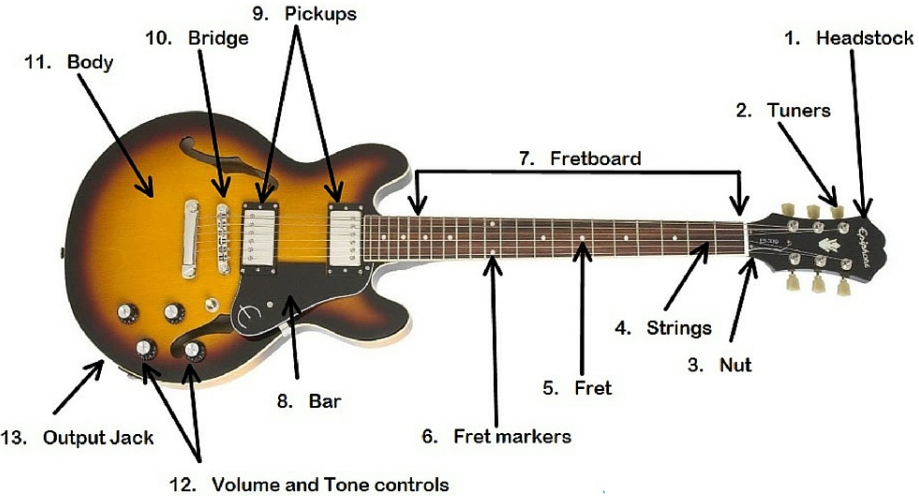
\includegraphics[width=0.9\textwidth]{guitar_parts.png}
		\caption{Illustration of an electric guitar and its parts \cite{coustii}.}
		\label{fig:guitar_parts}
\end{figure}
\todo[inline]{Sebastian: Maybe remove blue box?}

In the figure several parts are highlighted, but not all of them influence the sound, in the case where the guitar is not amplified. The pickups, the volume and the tone control have a large influence on the sound, when amplified, but they have no influence when not amplified. The Tuners do have an influence on the sound, but more in the sense of making sure the guitar is in tune, which also is more or less the case with the fretboard. 
The parameters that will be investigated and have an influence on the sound, when not amplified, are:

\begin{itemize}
 \item String thickness and material
 \item String action
 \item Bridges
\end{itemize}

\subsection{String thickness and material}
String thickness (gauge) affects the sound of a guitar a lot. String gauge affects the tone of the sound and the sustain of the sound. Tone is a very broad term, which says something about how a string sounds. Often tone is described in subjective terms such as warm, deep, crunchy etc \cite{premierguitar}. Sustain describes the period from when a tone is played until it fades out. Thicker strings will increase the sustain compared to thinner ones. Thicker strings will also increase the volume compared to thinner ones \cite{Helsinki}.
The material of the string also have an effect on its sound. Some of the materials used for electric guitar strings are: Nickel-plated steel, pure nickel and Stainless steel. Describing how the string material affects the sound is also often done in similar terms as for describing tone. E-Home Recording Studio fx. describes Nickel-plated steel as follows:
\\*
\\*
\textit{"Nickel-Plated Steel – which has a good combination of warmth and brightness, a strong picking attack, and is the most popular option."}\cite{E-Home}

\subsection{String action}
String action describes the distance from the strings to the fretboard on a guitar. A higher action allows the strings to vibrate more freely, and thereby increasing the sustain of the tone \cite{sweetwater}. If the string action is set too low, distortion can occur when a note is tapped.  

\subsection{Bridges}
The bridge on an electric guitar is where the playable area of the guitar strings begin. The purpose of the bridge is to keep the strings fixed on the body, but without adding too much friction to the strings. This is because it is wanted to transfer as less string vibration to the bridge as possible. Two main categories of electrical guitar bridges exist: the fixed bridges and the moving bridges. The type of bridge has an effect on several aspects when playing the guitar, but it is the string-friction on the bridge that has the largest effect on the sound \cite{seymourduncan}.
\\*
\\*
Other physical parts on an electric guitar such as the fretboard, the nut and the body does have an effect on the not amplified sound, because some of the string vibration will be transferred to these parts. These parts are however parts that are difficult to change, without decreasing the quality set by the factory.   


\todo[inline] {Sebastian: We need to explain the difference between the two volume control and tone control types}




 \section{Pickups on an electric guitar}
One of the most important parts of an electric guitar, is the transducer which converts the strings vibrations into an electrical signal. This is done with pickups, which as seen in \autoref{fig:guitar_parts}, is placed on the body. Typically an electric guitar has two or three pickups and the type and combination of pickups can vary. Two types of pickups are the single coil pickups and the dual coil (Humbucker) pickups. The electric equivalent to a single coil pickup is shown in \autoref{fig:electric_pickup}

\begin{figure}[h!]
\centering
\begin{circuitikz}\draw (0,0)
to[L=$L$]  (3,0)
to[R=$R$] (5,0)
(5,-1)to[short,-o](6,-1)
(5,0)to[short](5,-2)
to[C=$C$] (0,-2)
(0,-1)to[short,-o](-1,-1)
(0,-2)to[short] (0,0)
%to[short] (0,0)
;\end{circuitikz}
\caption{Electric equivalent of a single coil pickup \citep{build_your_guitar}.}
\label{fig:electric_pickup}
\end{figure}

A single coil pickup can be described as a an ideal inductor and a resistor in series, in parallel with a capacitor. This circuit is for the case when the guitars strings doesn't vibrate. When one or more strings are played, the circuit is expanded as shown in \autoref{fig:electric_pickup_strings}.

\begin{figure}[h!]
\centering
\begin{circuitikz}\draw (0,0)
to[L=$L$]  (3,0)
to[R=$R$] (5,0)
to[short, -o](6,0)
(5,0)to[C=$C$] (5,-2)
(6,-2)to[short, o-] (0,-2)
to[sV=$String$] (0,0)
%to[short] (0,0)
;\end{circuitikz}
\caption{Electric equivalent of a single coil pickup, when strings are played \citep{build_your_guitar}.}
\label{fig:electric_pickup_strings}
\end{figure}

When the strings are vibrates, they act as an \gls{ac} supply. The output signal from the pickup is then the voltage over the capacitor  \citep{build_your_guitar}. 
The complete circuit in an electric guitar is a bit more complicated, since an electric guitar often contains a volume control, one or more tone controls etc. A simple circuit of an electric guitar with one volume control and one tone control, is shown in \autoref{}

\begin{figure}[h!]
\centering
\begin{circuitikz}\draw (0,0)
to[L=$Pickup$]  (0,4)
to[short] (2,4)
to[vR=$Tone$ $pot$] (2,2)
to[C=$Tone$ $C$] (2,0)
to[short](0,0)
(2,4) to[short](5,4)
to[pR=$ $](5,0)
to[short](2,0)node[ground]{}
%Jack
(5.3,2)to[short]node[left,above]{$Volume$ $pot$}(6.6,2)
to[short](6.9,1.7)
to[short](7.2,2)
(7.5,2)to[short](7.5,1)
to[short](6,1)
to[short](6,0)
to[short](5,0)
(7.5,2)to[short](7.7,2)
to[short]node[right]{$Jack$ $input$}(7.7,1)
to[short](7.5,1)
%end Jack
;\end{circuitikz}
\caption{Simple circuit of an electric guitar with one volume control and one tone control \citep{electricalfun}.}
\label{fig:simple_guitar_circuit}
\end{figure}

The tone control is a simple lowpass filter and the volume control is a potentiometer. 

\subsection{Output impedance of an electric guitar}
A test was made to find the output impedance of an electric guitar. The test was made on a Fender Squier Classic Vibe Telecaster, and was tested with three pickup settings. The complete test journal can be seen in \autoref{app:output_impedance}. In \autoref{tab:impedance_test} the results from the output impedance test on the guitar is shown.

\begin{longtable}[h!]{ |m{\dimexpr 0.34\linewidth-2\tabcolsep}| 
          m{\dimexpr 0.33\linewidth-2\tabcolsep}| 
          m{\dimexpr 0.33\linewidth-2\tabcolsep}|   } 
\caption{Results from output impedance test of an electric guitar.} \label{tab:impedance_test} \\ 
 
\hline 
%%%%%%%%  
\textbf{Pickup setting} & \textbf{Minimum output impedance} & \textbf{Maximum output impedance} \\ 
%%%%%%%% 
\hline 
\endfirsthead     
\multicolumn{3}{c}{{{\footnotesize \bfseries \tablename\ \thetable{} -- Continued from previous page.}}} \\  
\hline 
%%%%%%%%  
\textbf{Pickup setting} & \textbf{Minimum output impedance} & \textbf{Maximum output impedance} \\ 
%%%%%%%%  
\hline 
\endhead       
\hline \multicolumn{3}{|r|}{{Continues on next page.}} \\ \hline 
\endfoot     
\hline 
\endlastfoot 
%%%%%%%% Content of table 
Neck & \SI{6220}{\ohm} at \SI{10}{\hertz} & \SI{58,51}{\kilo\ohm} at \SI{5167}{\hertz} \\ \hline
Bridge & \SI{7863}{\ohm} at \SI{10}{\hertz}  & \SI{73.06}{\kilo\ohm} at \SI{4010}{\hertz}\\ \hline
Neck and bridge & \SI{3563}{\ohm} at \SI{10}{\hertz} & \SI{53.43}{\kilo\ohm} at \SI{5702}{\hertz}\\ \hline
\end{longtable}

\subsection{Frequency area of an electric guitar}
A test was made to see which frequencies can be played on an electric guitar. The test was made with a Fender Squier Classic Vibe Telecaster, and was tested with two pickup settings. The complete test journal can be seen in \autoref{app:frequency_area}. In \autoref{tab:impedance_test} the results from the frequency spectrum test on the guitar is shown.

\begin{longtable}[h!]{ |m{\dimexpr 0.34\linewidth-2\tabcolsep}| 
          m{\dimexpr 0.33\linewidth-2\tabcolsep}| 
          m{\dimexpr 0.33\linewidth-2\tabcolsep}|   } 
\caption{Results from output impedance test of an electric guitar.} \label{tab:impedance_test} \\ 
 
\hline 
%%%%%%%%  
\textbf{Pickup setting} & \textbf{Lowest significant frequency} & \textbf{Highest significant frequency} \\ 
%%%%%%%% 
\hline 
\endfirsthead     
\multicolumn{3}{c}{{{\footnotesize \bfseries \tablename\ \thetable{} -- Continued from previous page.}}} \\  
\hline 
%%%%%%%%  
\textbf{Pickup setting} & \textbf{Lowest significant frequency} & \textbf{Highest significant frequency} \\ 
%%%%%%%%  
\hline 
\endhead       
\hline \multicolumn{3}{|r|}{{Continues on next page.}} \\ \hline 
\endfoot     
\hline 
\endlastfoot 
%%%%%%%% Content of table 
Neck & Around \SI{80}{\hertz} & Around \SI{4400}{\hertz} \\ \hline
Bridge & Around \SI{80}{\hertz}  & Around \SI{4400}{\hertz}\\ \hline
\end{longtable}




\section{Effect on an electric guitar}

Electrical guitars can have more effects than the ones that can be done with the physical part. Those additional ones will be described in the following part. The ones that are going to be described are:

\begin{itemize}
 \item Equalizing
 \item Reverberation
 \item Overdrive
 \item Distortion
 \item Chorus
 \item Flanger
 \item Wah-Wah
\end{itemize}


\newpage

\input{chapters/analysing/equalizing}\label{sec:equalizing} 
\subsection{Delay}
Delay is an audio effect which memorizes the input signal for a customized time, and then release it without changing anything else than the amplitude. The delayed signal can either be played back multiple times or only once . When the signal is delayed and then played back multiple times, it can either be amplified or attenuated. If the delayed signal is amplified, it will start to oscillate. If the wanted effect is an echo, the delayed signal shouldn't be kept alive, then the gain in the feedback must be reduced in order to attenuate the signal.  \autoref{fig:delay_block} shows a block diagram of a simple delay, "echo" unit.


\begin{figure} [htbp]
 \centering
\begin{picture}(0,0)%
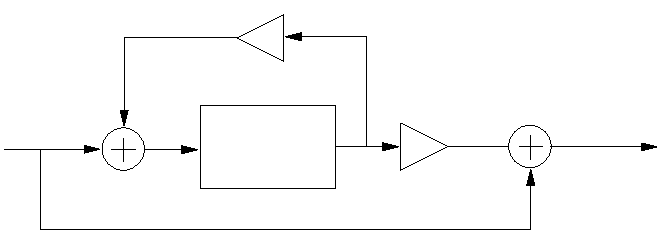
\includegraphics{delay.pdf}%
\end{picture}%
\setlength{\unitlength}{4144sp}%
%
\begingroup\makeatletter\ifx\SetFigFont\undefined%
\gdef\SetFigFont#1#2#3#4#5{%
	\reset@font\fontsize{#1}{#2pt}%
	\fontfamily{#3}\fontseries{#4}\fontshape{#5}%
	\selectfont}%
\fi\endgroup%
\begin{picture}(5035,1329)(1491,-118)
\put(4726,704){$Gain$}%

\put(3106,479){$Delay$}%

\put(5814,672){$Output$}%

\put(1506,659){$Input$}%

\end{picture}%

  \caption{The photo shows a block diagram on a delay unit \citep{delay_block}}
  \label{fig:delay_block}
\end{figure}

The block diagram \autoref{fig:delay_block} shows a delay unit with a feedback line that has an adjustable gain. The feedback signal is either attenuated or amplified depending on the gain value and then added to the delay line input \cite{delay_echo}. The following \autoref{fig:delay_echo} shows the effect in time domain.

\begin{figure} [htbp]
 \centering
  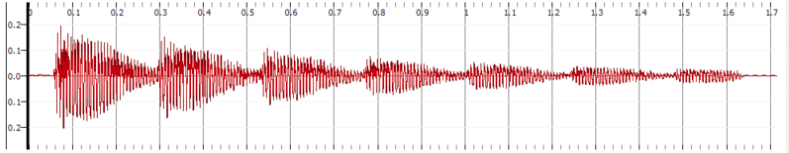
\includegraphics[width=1\textwidth]{delay_echo}
  \caption{The photo shows a echo in time domain}
  \label{fig:delay_echo}
\end{figure}
\todo[inline]{make figure i matlab}

The \autoref{fig:delay_echo} shows that the main signal is repeated and attenuated 6 time before it is totally attenuated. A time domain diagram is shown at \autoref{fig:delay_timed}.

\begin{figure} [htbp]
 \centering
\begin{picture}(0,0)%
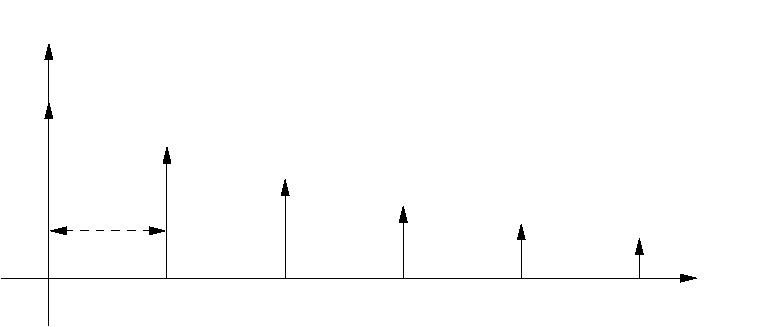
\includegraphics{delay_timed.pdf}%
\end{picture}%
\setlength{\unitlength}{4144sp}%
%
\begingroup\makeatletter\ifx\SetFigFont\undefined%
\gdef\SetFigFont#1#2#3#4#5{%
  \reset@font\fontsize{#1}{#2pt}%
  \fontfamily{#3}\fontseries{#4}\fontshape{#5}%
  \selectfont}%
\fi\endgroup%
\begin{picture}(5843,2478)(4129,-5833)
\put(9496,-5506){$Time$}%
\put(4231,-3526){$Magnitude$}%
\put(4591,-4291){$Main$}%
\put(5536,-4606){$G$}%
\put(6436,-4876){$G^2$}%
\put(7336,-5056){$G^3$}%
\put(8236,-5191){$G^4$}%
\put(9136,-5281){$G^5$}%
\put(4861,-5056){$t\Delta$}%
\put(6256,-5776){$t2$}%
\put(5356,-5776){$t1$}%
\put(7156,-5776){$t4$}%
\put(8056,-5776){$t5$}%
\put(8956,-5776){$t6$}%
\end{picture}%
  \caption{The figure shows the impulse respond of the delay unit}
  \label{fig:delay_timed}
\end{figure}
\label{sec:delay} 
\section{Reverberation}
Reverberation is \label{sec:reverberation} 
\subsection{Overdrive and Distortion} 

The distortion effects changes the sound of the played instrument by increasing the gain. It is commonly used the with the electric guitar. The sound changes due to the clipping effect. \\
\todo[inline]{Muhammed: "It is commonly used in the with the electric guitar" does something missing?}

The clipping effect is a way of changing the waveform when an amplifier is over driven; forcing it to deliver an output that is higher than its maximum capability. \\
The part of the waveform where the amplifier is asked to get a value higher than its maximum capacity gets the maximum value the amplifier can give. It means that all the parts of the waveform where the amplifier is pushed more than its capacity will have the same amplitude. The signal is then 'clipped'. An illustration of this effect is shown in \autoref{fig:clipping1}.\\

\begin{figure} [htbp]
	\centering
  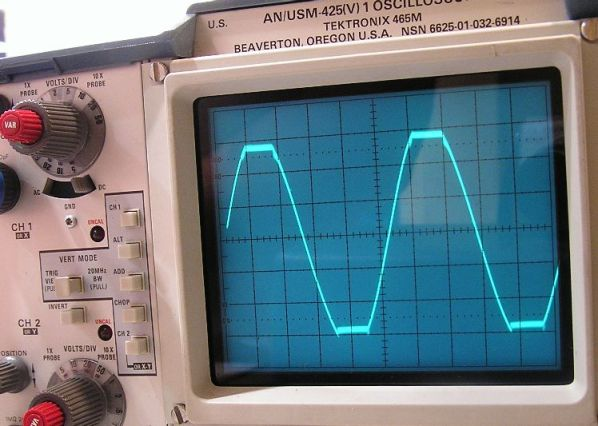
\includegraphics[width=0.7\textwidth]{clippingeffect.jpg}
  \caption{Photo showing the effect of clipping, a consequence of the overdrive or distortion effect.}
  \label{fig:clipping1}
\end{figure}


The consequences in the frequency domain are that the clipping effect creates more harmonics at high frequency than the signal without the clipping effect. \\

The clipping effect in signal processing happens when the amplitude is limited by a number and if during the processing the amplitude surpasses this limit, clipping happens because the value is then maxed to the maximum number that can be handled digitally. The maximum amplitude that can be handled is determined by the number of bits the system uses. The maximum number for a \SI{16}{\bit}  signed integers system is $\frac{2^{16}}{2} = \SI{32768}{\cdot}$ which means that if a value has an amplitude higher than this number the clipping effect occurs. \\

In any clipping technique, there is a creation of new harmonics. In the case of soft clipping, the new harmonics are multiples of the harmonics of the original tone. Valve Overdrive is a soft clipping technique for instance. In the case of hard clipping, they are not multiples which results to what is called intermodulation. Hard clipping usually happens when the harmonics of the original signal are not related by a multiple. Transistor overdrive is an example of hard clipping.  Effects of hard and soft clipping on the waveforms are shown in \autoref{fig:clipping2}.

In the previous paragraphs, distortion and overdrive has been explained as if they are the same effects. In fact, there is a small difference between the two. Distortion changes the original tone more than overdrive which means that distortion will generate more extra harmonics than overdrive and their amplitude tend to be higher. Overdrive effect has "cleaner" consequences on the final tone than distortion. Overdrive is often assigned to soft clipping while distortion is assigned to hard clipping.

\begin{figure} [htbp]
	\centering
  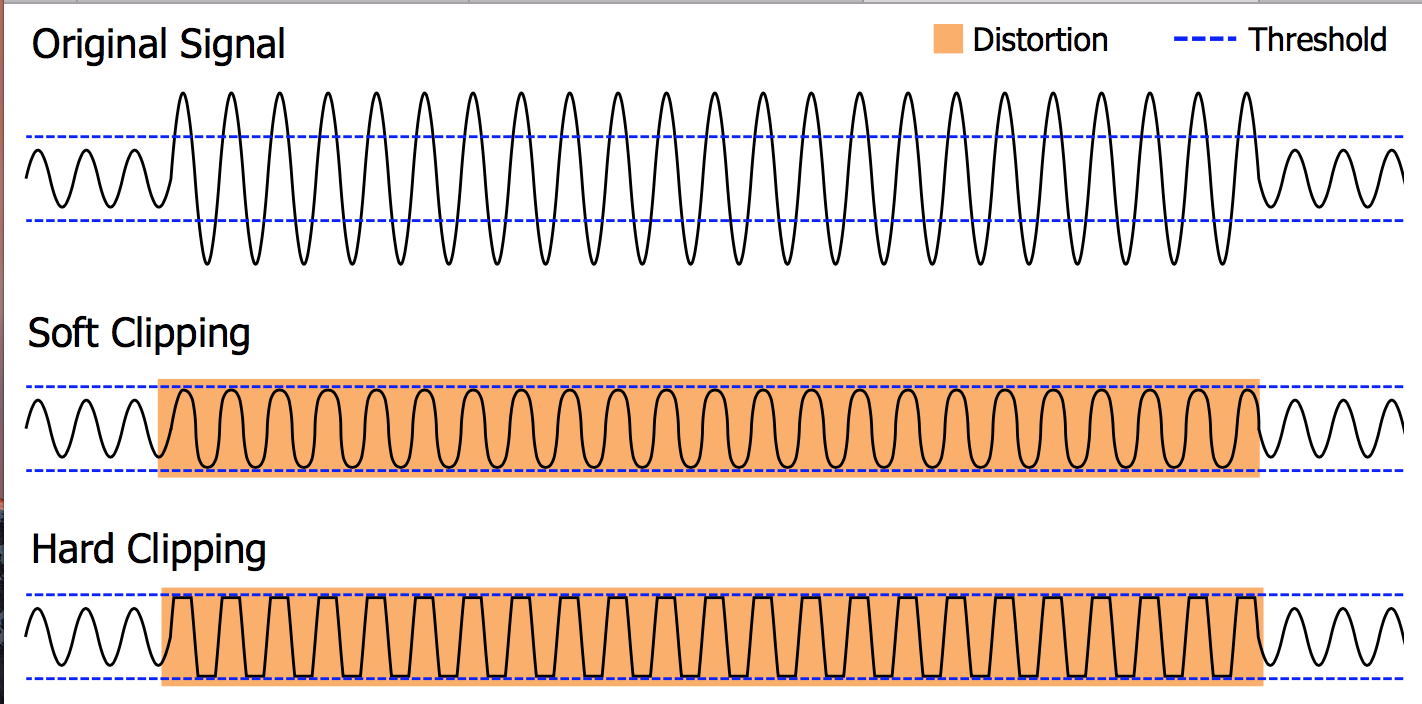
\includegraphics[width=0.7\textwidth]{softhardclipping.png}
  \caption{Photo showing the effect of hard and soft clipping, a consequence of the overdrive or distortion effect.}
  \label{fig:clipping2}
\end{figure}


\label{sec:overdrive} 
\subsection{Chorus and Flanger Effect} \label{sec:chorus} 

%\label{chor_flang}

The chorus effect is obtained when a signal is delayed and then mixed with its original version \citep{chorus_gibson} \citep{chorus_apple}. \\
The chorus effect takes a single audio signal as input and applies different delay values to it. Chorus effect using one delay is called flanger. Each of the delayed signals are then mixed with the original audio input. \\
A \gls{lfo} can be used to make the delay times vary. Different \gls{lfo}s can be used for each of the delay channels to make a richer sound mix and avoiding repetitive sound but it implies more computations. The same \gls{lfo} can be used for all the delay channels but not at the same cycle for each delay \citep{chorus_testtone}. \\ 

Different parameters on the chorus effect can changed by settings on the hardware. Some of these are:\\
\begin{itemize}
\item \textbf{Delay time}: The time difference between the original sound and the delayed one (The frequency of the signal from the \gls{lfo}).
\item \textbf{Chorus size}: The number of delayed sounds that will be mixed.
\item \textbf{Depth}: The amplitude of the signal from the \gls{lfo}.
\item \textbf{Waveform}: The waveform of the signal from the \gls{lfo} can be changed to triangle, sine, log ect. \citep{hobby_hour_chorus}
\item \textbf{Gain}: The amplification of the delayed signal.
\end{itemize} \citep{chorus_parameters}

A block diagram for  the chorus and flanger effect is shown in \autoref{fig:chorus_diag}.

\begin{figure} [htbp!]
	\centering
\begin{picture}(0,0)%
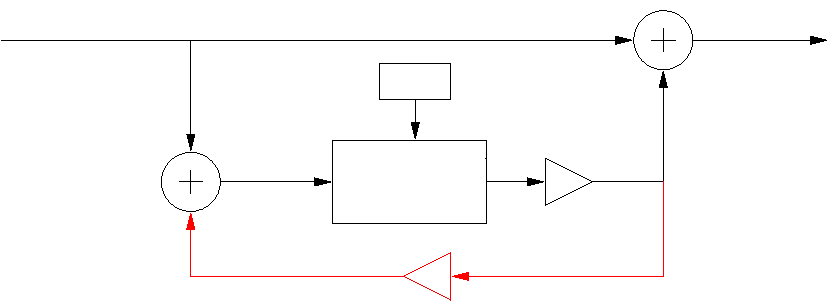
\includegraphics{chorus_diag.pdf}%
\end{picture}%
\setlength{\unitlength}{4144sp}%
%
\begingroup\makeatletter\ifx\SetFigFont\undefined%
\gdef\SetFigFont#1#2#3#4#5{%
	\reset@font\fontsize{#1}{#2pt}%
	\fontfamily{#3}\fontseries{#4}\fontshape{#5}%
	\selectfont}%
\fi\endgroup%
\begin{picture}(6327,3018)(3766,-3493)
\put(6706,-1366){\color[rgb]{0,0,0}LFO}%

\put(8101,-1636){\color[rgb]{0,0,0}Gain}%

\put(3781,-646){\color[rgb]{0,0,0}Input}%

\put(9406,-646){\color[rgb]{0,0,0}Output}%

\put(6571,-1906){\color[rgb]{0,0,0}Delay}%

\put(6616,-3211){\color[rgb]{1,0,0}Delay}%

\put(8101,-2986){\color[rgb]{1,0,0}Gain}%

\put(6706,-2671){\color[rgb]{1,0,0}LFO}%

\end{picture}%



\caption{Block Diagram of the chorus effect.}
\label{fig:chorus_diag}
\end{figure}


As it can be seen on the block diagram in figure \autoref{fig:chorus_diag}, a signal that hasn't been affected by any changes is added to the same signal delayed, controlled by the \gls{lfo}. The addition is done just before the output. The chorus effect is represented by the black and the red parts of the block diagram. The flanger effect is represented only by the black parts of the block diagram. In \autoref{fig:chorus_and_flanger_time} the impulse response of the chorus and the flanger effect are shown. Its is seen that with a pulse as the input, in the flanger effect, the output will be the original pulse, followed by an echo. The period before this echo arrives varies, based on the \gls{lfo}. When using the chorus effect several echoes will arrive, still with varying delay time. 

\begin{figure}[htbp!]
\centering
\def\svgwidth{\columnwidth}
\scalebox{0.8}{\input{figures/analysing/chorus_and_flanger_time_domain.pdf_tex}}
\caption{Impulse response of the flanger effect (black) and the chorus effect (red).}
		\label{fig:chorus_and_flanger_time}
\end{figure}










\label{sec:chorus} 
\subsection{Wah-Wah}\label{sec:wah-wah} 

The effect takes the original signal and mix it with another signal that passes through a bandpass filter. The bandpass filter is time varying, which means that it changes its position in the frequency spectrum \citep{wah-wah_course}. \\
The automatic Wah-Wah effect have some different parameters that can be changed to customize the effect:\\

\begin{itemize}
	\item \textbf{The \gls{lfo} frequency}: it sets the speed at which the bandpass filter moves in the frequency spectrum.
	\item \textbf{\gls{lfo} start phase}: Determine where should the bandpass filter start.
	\item \textbf{\gls{lfo} depth}: the range of frequencies it should work on, high depth gives a bigger range and vice versa.
\end{itemize} \citep{wah-wah_audacity}

A block diagram of the effect is illustrated in \autoref{fig:wah_diag}.  

\begin{figure} [htbp]
	\centering
\begin{picture}(0,0)%
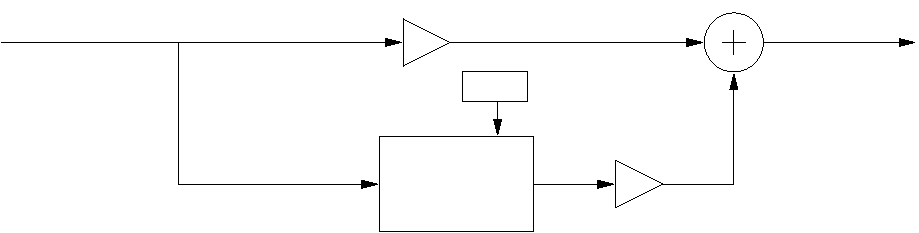
\includegraphics{wah_diag.pdf}%
\end{picture}%
\setlength{\unitlength}{4144sp}%
%
\begingroup\makeatletter\ifx\SetFigFont\undefined%
\gdef\SetFigFont#1#2#3#4#5{%
  \reset@font\fontsize{#1}{#2pt}%
  \fontfamily{#3}\fontseries{#4}\fontshape{#5}%
  \selectfont}%
\fi\endgroup%
\begin{picture}(6999,1770)(2689,-2233)
\put(6841,-1591){\textit{Wah-Wah Gain}}%
\put(5626,-2041){$Filter$}%
\put(6136,-1186){\textit{LFO or Pedal}}%
\put(2746,-646){$Input$}%
\put(8686,-646){$Output$}%
\put(5626,-1816){$Bandpass-$}%
\put(5986,-646){$Gain$}%
\end{picture}%
	\caption{Block diagram of the wah-wah effect}
	\label{fig:wah_diag}
\end{figure}

It can be seen on the block diagram that the filtered signal is added to the direct signal. Thus, this block diagram is a representation of the wah-wah effect.  \\


The phaser effect can be created by using a band-stop filter instead of a bandpass filter using the same block diagram presented in \autoref{fig:wah_diag} \citep{wah-wah_cardiff}. \\

There is another type of wah-wah effect called M-fold wah-wah which uses multiple M-tap bandpass filters that move around the spectrum at the same time \citep{wah-wah_cardiff}. \\

An example of a time domain response is shown in figure \autoref{fig:wah-wah-response}. \\

\begin{figure} [htbp!]
	\centering
	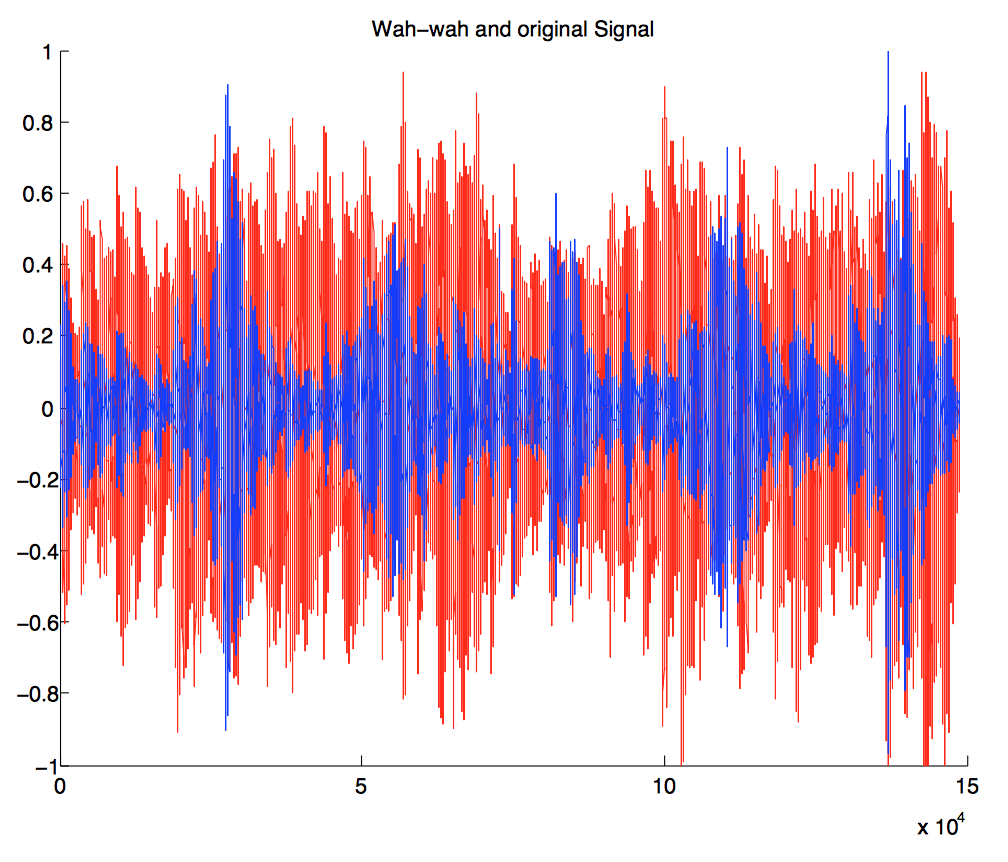
\includegraphics[width=0.6\textwidth]{wah-wah-response.png}
	\caption{Time domain response of the original sound (red) and the one after having the wah-wah effect (blue) \citep{wah-wah_cardiff}.}
	\label{fig:wah-wah-response}
\end{figure}
\todo[inline]{write about wah wah frequency in text}

\todo[inline]{Jonas: Muhammed, can you explain the above time domain spectra?(and the block diagram)}
\todo[inline]{Sebastian: Maybe make figure our self, because axis descriptions are missing now}

As it can be seen on \autoref{fig:wah-wah-response}, the wah-wah effect reduced the amplitudes of many parts of the wave-form compared to the signal without the wah-wah effect. Some of the them remained the same. It is due to the bandpass-filtering.
In \autoref{fig:wah_wah_frequency} an illustration of the bandpass filter in the wah-wah effect in frequency domain is shown. 

\begin{figure}
\centering
\def\svgwidth{\columnwidth}
\input{figures/analysing/wah_wah_frequency_domain.pdf_tex}
\caption{Frequency domain illustration of bandpass filter in the wah-wah effect}
		\label{fig:wah_wah_frequency}
\end{figure}

It is shown that the bandpass filter can be moved in frequency. This movement is done either by an \gls{lfo} or with an expression pedal.
\label{sec:wah-wah} 

\section{Platform comparing}
In order to implement the previous discussed effects digitally, a platform has to be chosen. In this section a list of possible platforms for the effect implementation will be analysed. The following platforms will be analysed:

\begin{itemize}
\item Rasperry pi
\item \gls{dsp}
\item \gls{fpga}
\end{itemize}

\subsection{Raspberry pi}
There exist different generations of the Raspberry pi, but the one that will be analysed is the Raspberry pi 3 model B, since it is the latest version. 
A Raspberry pi is a \gls{sbc} at the size of a credit-card. A picture of the Raspberry pi 3 model B, is shown in \autoref{fig:RP3mB}.

\begin{figure}[h]
	\centering
		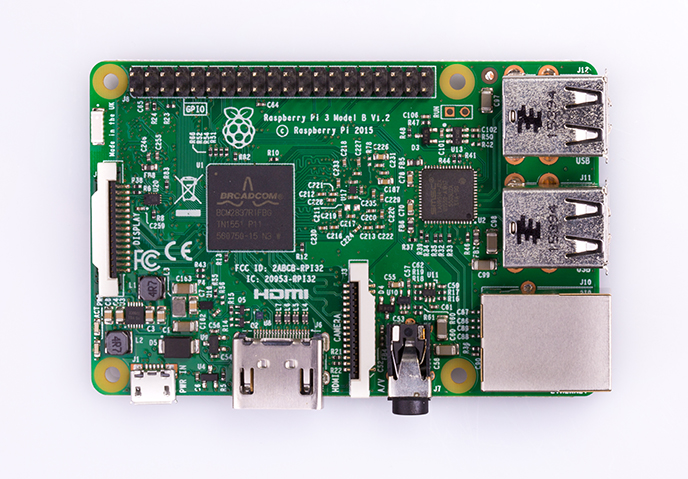
\includegraphics[width=0.7\textwidth]{Raspberry_pi_3_model_B.jpg}
		\caption{Picture of the Raspberry Pi 3 model B \cite{Raspberry_pi}.}
		\label{fig:RP3mB}
\end{figure}

The Raspberry pi 3 model B has a 1.2 GHz Quad-core ARM processor, supports wireless LAN and Bluetooth 4.1. It has 1GB RAM and has connectors for micro SD cards \cite{Raspberry_pi}.
The Raspberry Pi is Linux based, but can also run Windows \cite{sparkfun_Raspberry_pi}. This makes the Raspberry pi 3 model B suited for a wide range of projects. This is both its advantage and its disadvantage if a specialized platform is wanted. 

\subsection{Digital Signal Processor}
A \gls{dsp} is a processor, which is optimized for high-speed numerical operations such as: Addition, subtraction and multiplication. A typical \gls{dsp} system includes an anti-aliasing filter, an \gls{adc}, a \gls{dsp}, a host interface, a \gls{dac} and a anti-imaging filter. A block diagram of the typical \gls{dsp} system is shown in \autoref{fig:typ_dsp}.

\begin{figure}
\centering
\def\svgwidth{\columnwidth}
\input{figures/analysing/DSP_typical.pdf_tex}
\caption{Block diagram of a typical \gls{dsp} \cite{AnalogDialogue}.}
		\label{fig:typ_dsp}
\end{figure}

These high-speed numerical operations make the \gls{dsp} suited for real-time applications, and a \gls{dsp} can work both as a sample-based system and as a frame-based system. 
Two terms are commonly used for describing the processing power of a \gls{dsp}. These are \gls{mips} and \gls{mops}. The requirements of the \gls{dsp} can be found, based on the sampling interval and the number of operations needed between each sample. This is shown in \eqref{eq:MOPS}.

\begin{equation}\label{eq:MOPS}
        DSP_{speed} = \frac{Operations}{T_s}\addunit{MOPS}
    \end{equation}

    \startexplain
        \explain{$DSP_{speed}$ is the \gls{dsp}'s processing power}{MOPS}
        \explain{$Operations$  is the number of operations}{1}
        \explain{$T_s$ is the sampling interval}{\si{\second}}
    \stopexplain


\gls{mips} and \gls{mops} are not the same, but related in the way that each \gls{dsp} instruction containe a numbers for operation  \cite{AnalogDialogue}. E.g. a \gls{dsp} with 4 \gls{mips} and 8 \gls{mops} means that the \gls{dsp} can preform 2 operation for each instruction.


\label{sec:platform_comparing}
\subsection{FPGA}


The FPGA (Field Programmable Gate Array) is a circuit that contains multiple logic blocks and routing channels.\\
The hardware configuration is customizable in order to meet the user’s demands in the digital domain; unlike ICs where the connections between the transistors cannot be changed, it is possible to make a custom architecture on an FPGA. \\
As said, the FPGA consists of multiple logic blocks often called logic cells. Each cells consists of an LUT (Look-up table) and a flip-flop. The LUT has four inputs and the flip-flop one clock input. The LUT contains a small Random Access Memory and performs logical operation. \\
Around the logic blocks, there are multiple I/O blocks which can also be programmed to an output or input for instance.  \\
An FPGA contains a configuration logic that is connected to the flash memory which contains information about the connection between the logic blocks and the architecture inside the block itself. The more logic blocks are used and programmed, the bigger the flash memory storage size has to be. An overview of the structure of the FPGA is shown in \autoref{fig:fpgastructure} and the structure of the logic block in \autoref{fig:logicblockstruct}. \\
\newline

\begin{figure}[htbp]
	\centering
	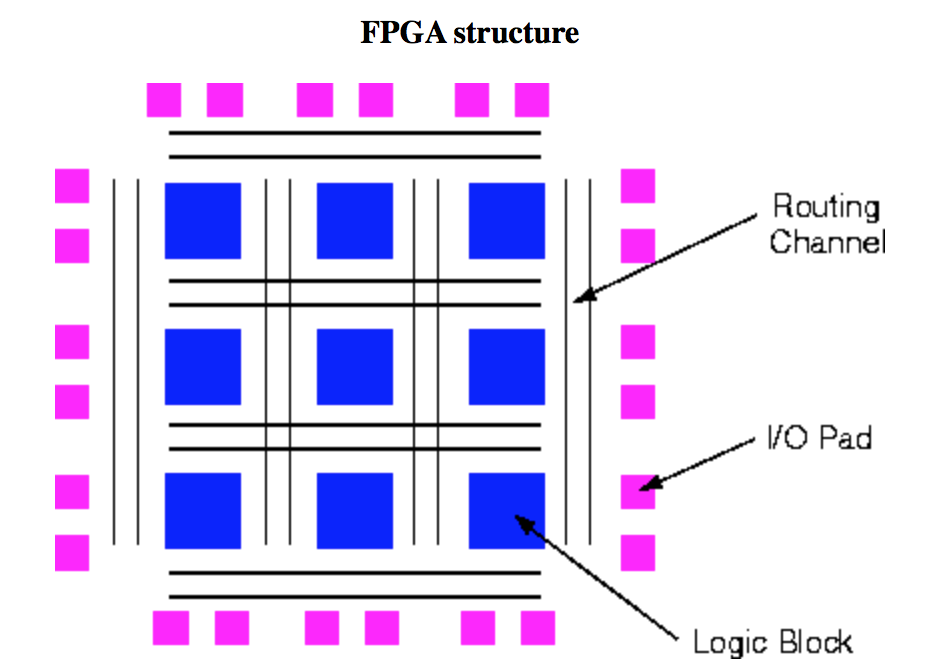
\includegraphics[width=0.7\textwidth]{fpgastructure}
	\caption{Scheme of FPGA components.}
	\label{fig:fpgastructure}
\end{figure}

\begin{figure}[htbp]
	\centering
	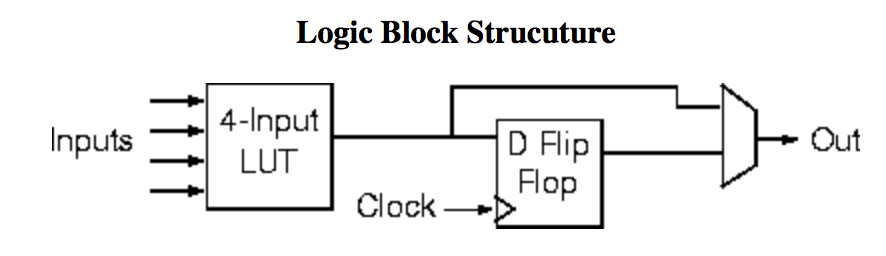
\includegraphics[width=0.7\textwidth]{logicblockstruct}
	\caption{Structure of a logic block.}
	\label{fig:logicblockstruct}
\end{figure}


The biggest advantage of the FPGA is to make multiple processes at the same time by isolating some logic blocks and I/Os for a specific task, which is not possible with ICs. A micro controller needs to run tasks in sequence, one after the other. If different tasks needs to be done in a restricted timing, this parameter can be crucial. 
By using parallelism and having fast I/Os, the FPGA can be very powerful. \\

The FPGA can be programmed using a hardware description language like VHDL or Verilog. \\

FPGA are certainly more efficient than ICs and normal micro controller but they are also more expensive especially if it’s about cloning a pre-existing micro controller without any personal added value. They are also power demanding. The FPGA has a configuration flash memory which means that there is no need for the user to intervene after a reboot, but at each boot the FPGA is programmed from scratch using the data from the flash memory which can drastically increase the boot time as well as the power consumption. It is more complicated to program an FPGA than using an IC or micro controller because it has to be designed by the user. \\








 \label{sec:FPGA}
\section{The benefits of using digital signal processing over analog}
\subsection{Quality}

The bandwidth in an analog sound signal can be increased infinitely unlike the digital one where it is limited by the sampling rate that is being used. \\

The quality in the digital signal is  lower because in the digital domain there is what is called the digital noise. It occurs after sampling, and increase when the sound between samples get less and less smooth. On the other side, in the analog domain, the signal is not sampled, it is the real one so this problem do not exist. Errors can also occur due to bit depth, bit depth limits the values that the sample can take, which means that even with high sample rate but low bit depth, the digital track can sound different. The number of values that can be sampled is defined by the number of bits per sample, and the number of values are then $2^{number of bits}$ \citep{analog_quality}.\\
It can then be inferred that there are quantization noise and errors in digital signals, which do not exist in analog signals. The same goes for aliasing \citep{analog_aliasing}. 

\subsection{Mobility}

Digital Sounds are more portable than analog ones, they can be played on different machines and copied without losing any information unlike the analog sound that can only be played on a tape for instance \citep{analog_quality}. 

\subsection{Lifetime}

A digital sound can last longer than an analog one. A Vinyl disk for example can get damaged and impact the sound stored on it and thus the quality. On the other side, a digital file saved on a computer cannot get damaged physically, unless the storage does, and can be duplicated very easily to preserve it. With the rise of cloud systems, the loss of a digital file is nearly impossible unless intentional \citep{analog_storage}.


\subsection{Requirements}

It is easier to fulfil given requirements using digital over analog signal processing because the user has more control over the digital controller than the analog one. If at anytime, the engineer realizes that the components needs more processing power, it can be easily upgraded \citep{analog_requirements}.

\subsection{Functionality and Customization}

With only one \gls{dsp}, it is possible to program numerous effects, personalize them and even create custom ones. Effects presented in \autoref{sec:effects} are just part of a growing and endless world of digital effects. 

  \label{sec:digital_vs_analog}
\chapter{Problem Analysis Conclusion}\label{ch:analysing_cl}
In the previous \autoref{ch:analysing}, different sound personalizations that can be done without any effect pedals on an electric guitar has been scrutinized. Then, different effects in the digital domain has been presented followed by the advantages of digital signal processing over analog. Different devices for \gls{dsp} have also been presented.  \\
\newline
It can be inferred from the analysis \autoref{sec:electric_guitar_theory} that the level of customization when using the physical part of the guitar is very low. However, there is a great number of effects that can be attached to this type of guitars and give the musician more possibilities, some of them presented in \autoref{sec:effects}.  \\
During the last decades, a lot of improvements have been made in the digital domain. The digital sound quality is now comparable to the analog one even for an audiophile. The advantages of using analog signal processing over digital are getting weaker. On the other side, various reasons can push the user to choose digital over analog: portability, lifetime, personalization, ease of use...

\chapter{Problem statement}
Based on the knowledge found in the analysis, and the conclusions drawn from it, a problem statement can be made. The following problem statement will be the focus of the rest of the project:
\\
\\
\textbf{How can a number of digital guitar effects be designed and implemented using Digital Signal Processing?}
\section{Delimitations}
The following delimitations are made for the rest of the project:

\begin{itemize}
\item Since the main focus of this project will be to design and digitally implement guitar effects, the design of the analog parts of the project will, as often as possible, be done using \gls{ic}'s. 
\item It is chosen to work with mono audio, since this will be sufficient for the main focus of the project.
\end{itemize} 
 
\chapter{Product Requirements}
This chapter lists the requirements for the effects presented in the analysis. 

\begin{figure}[htbp]
	\centering
\begin{picture}(0,0)%
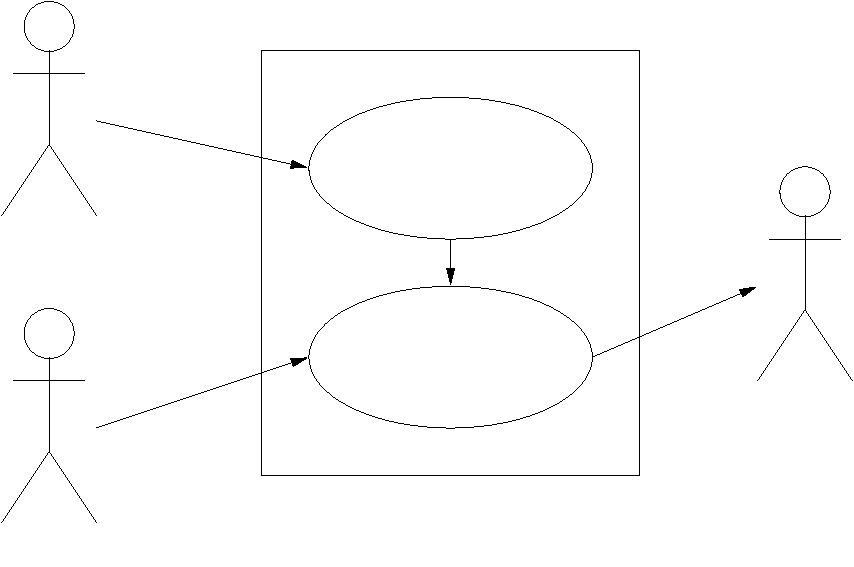
\includegraphics{Use_case.pdf}%
\end{picture}%
\setlength{\unitlength}{4144sp}%
%
\begingroup\makeatletter\ifx\SetFigFont\undefined%
\gdef\SetFigFont#1#2#3#4#5{%
  \reset@font\fontsize{#1}{#2pt}%
  \fontfamily{#3}\fontseries{#4}\fontshape{#5}%
  \selectfont}%
\fi\endgroup%
\begin{picture}(6507,4318)(1426,-4900)
\put(1531,-2491){User}%
\put(4546,-3346){Effect}%
\put(4276,-1906){Effect select}%
\put(7111,-3751){Amplifier}%
\put(1441,-4831){Guitar}%
\end{picture}%
	\caption{A graphically overview of wanted functionality in form of an use case digram.}
	\label{fig:use_case}
\end{figure}

From \autoref{ch:analysing} some of the effect can be designed together, because the effect is using the same parts but multiply times or just a small difference. The following description tells shortly about the different in the effect block and which effect that can be designed together.

\paragraph{Basic filtering}
The only basis filter, which is explained in \autoref{ch:analysing} which is a basic filter without delay and time changing parameters is the Equalizer.


\paragraph{Time varying filter}
The only Time varying filter, which is explained in \autoref{ch:analysing} is the Wah-Wah.


\paragraph{Delay}
All the delay based effect have at lest one delay block and have both fast and slow delay. All the analysed delayed based effect in \autoref{ch:analysing} is:
\begin{itemize}
	\item Delay
	\item Flanger
	\item Chorus
	\item \gls{reverb}
\end{itemize} 

The block diagram in each effect shows that two and two effect have a common structure with using the same parts but multiply times. In another way the chorus is the flanger with 

\paragraph{Non-linear processing}
\begin{itemize}
	\item Distortion
	\item Overdrive
\end{itemize} 

\subsection{Block}

The requirements are divided into units, based on the effect analysis \autoref{ch:analysing}, since it is concluded in \autoref{ch:analysing} that only six general units need to be designed and all the presented effects can be created with those six. The unit that are going to be designed are the:



\begin{itemize}
	\item Bandpass filter
	\item Inverse bandpass filter
	\item Delay
	\item Gain
	\item Clipping
	\item \gls{lfo}
\end{itemize} 

 Besides the fact that each unit shall be designed individually, each unit interface should fit in the effect that is using it. Each unit has its own section where the requirements and their arguments are presented. To ensure that the units can fit and work together, basic requirements  are made on the processing component to be chosen afterwards first.
 
 
\newcommand{\reqbasis}{The delay unit must delay the input signal, in time defined by external unit.}

\reqPrefix{BS}
\section{Basis requirements}
Based on the \autoref{ch:analysing}, the delay requirement is as following

\begin{requirement}\label{req:dsp}
    \requirement{The processing component module are used to process the signal }
    \argument{It is concluded that the effect shall be made digitally}
\end{requirement}

\begin{requirement}\label{req:software}
    \requirement{Each unit must fit into a \gls{dsp} architecture}
    \argument{In order to be able to design all unit digitally}
\end{requirement}

\begin{requirement}\label{req:speed}
    \requirement{The calculation of one effect shall be faster than the sample frequency. }
    \argument{The processing component shall be fast enough to calculate at lest one effect between two sample}
\end{requirement}


\newcommand{\reqconverters}{The delay unit must delay the input signal, in time defined by external unit.}

\reqPrefix{Converter}
\section{Converters}
Based on \autoref{sec:pickups}, the requirements for the \gls{adc} and the \gls{dac} are as follows:

\begin{requirement}\label{req:ADC_resolution}
    \requirement{The \gls{adc} much have a resolution of at least 10 bits.}
    \argument{This requirement is made according to \autoref{eq:dB_max_min_guitar_out}.}
\end{requirement}


\begin{requirement}\label{req:ADC_Fs}
    \requirement{The sampling frequency of the \gls{adc} must be at least \SI{8.8}{\kilo \hertz}. }
    \argument{This requirement is made according to \autoref{tab:frequency_area}.}
\end{requirement}

\begin{requirement}\label{req:DAC_resolution}
    \requirement{The \gls{dac} much have a resolution of at least 10 bits.}
    \argument{This requirement is made according to \autoref{eq:dB_max_min_guitar_out}.}
\end{requirement}

\begin{requirement}\label{req:DAC_Fs}
    \requirement{The sampling frequency of the \gls{dac} must be at least \SI{8.8}{\kilo \hertz}. }
    \argument{This requirement is made according to \autoref{tab:frequency_area}.}
\end{requirement}
%\newcommand{\reqbandpass}{The delay unit must delay the input signal, in time defined by external unit.}

\reqPrefix{EQ}
\section{Equalizer (\reqPrefixName)}
Based on \autoref{ch:analysing}, the following requirements are made for the equalizer:

\begin{requirement}\label{req:equalizer}
    \requirement{The gain of each individual band in the equalizer must be changeable by the user.}
    \argument{In order to give the user the possibility of equalizing the sound as wanted.}
\end{requirement}

\begin{requirement}\label{req:equalizer2}
    \requirement{Each band in the equalizer must, when fully amplified or fully attenuated, drop \SI{6}{\decibel} at the neighbouring bands center frequencies.}
    \argument{In order to make each band independent so the user can change one frequency area, without affecting the others.}
\end{requirement}

%%\newcommand{\reqgain}{The delay unit must delay the input signal, in time defined by external unit.}

\reqPrefix{Wah-Wah}
\section{Wah-Wah}
Based on \autoref{ch:analysing}, the following requirements are made for the Wah-Wah effect:

\begin{requirement}\label{req:WahWah}
    \requirement{The gain unit must be able to attenuate and amplify the input signal}
    \argument{In order to be able to create echo effects, clipping, and control the gain for delays}
\end{requirement}




%\newcommand{\reqclipping}{The delay unit must delay the input signal, in time defined by external unit.}

\reqPrefix{Reverb}
\section{Reverb}
Based on \autoref{ch:analysing}, the following requirements are made for the \gls{reverb} effect:

\begin{requirement}\label{req:reverb1}
    \requirement{The \gls{reverb} effect must at least produce 1000 echoes per second.}
    \argument{\citep{natural_sounding_revorb}.}
\end{requirement}

\begin{requirement}\label{req:reverb2}
    \requirement{The user must be able to change the ratio between the direct input and the output of the \gls{reverb} effect.}
    \argument{Design choice to make the effect flexible for the user.}
\end{requirement}

\begin{requirement}\label{req:reverb3}
    \requirement{The user must be able to increase the number of echoes per second.}
    \argument{Design choice to make the effect flexible for the user.}
\end{requirement}


%\newcommand{\reqdelay}{The delay unit must delay the input signal, in time defined by external unit.}

\reqPrefix{Delay}
\section{Delay}
Based on \autoref{ch:analysing}, the following requirements are made for the delay effect:

\begin{requirement}\label{req:delay1}
    \requirement{The delay effect must produce a specified number of echoes per second.}
    \argument{Functional requirement.}
\end{requirement}

\begin{requirement}\label{req:delay2}
    \requirement{The user must be able to change the number of echoes per second.}
    \argument{Design choice to make the effect flexible for the user.}
\end{requirement}


%\newcommand{\reqlfo}{The delay unit must delay the input signal, in time defined by external unit.}

\reqPrefix{Chorus}
\section{Chorus}
Based on \autoref{ch:analysing}, the following requirements are made for the chorus effect:

\begin{requirement}\label{req:chorus1}
    \requirement{The \gls{lfo} unit must have a frequency from \SI{0.1}{\hertz} to \SI{10}{\hertz}  }
    \argument{In order to be able to make a signal which is under the audibility range. }
\end{requirement}

\begin{requirement}\label{req:chorus2}
    \requirement{The \gls{lfo} unit shall be able to make sinus, triangle, squared and sawtooth waveforms.}
    \argument{In order to create different effects like chorus, flanger and wah-wah.}
\end{requirement}


%\newcommand{\reqInversebandpassfilter}{The delay unit must delay the input signal, in time defined by external unit.}

\reqPrefix{Flanger}
\section{Flanger}
Based on the \autoref{ch:analysing}, the following requirements are made for the flanger effect:

\begin{requirement}\label{req:flanger1}
    \requirement{The inverse bandpass filter unit must be able to attenuate the gain in its stop-band.}
    \argument{In order to be able to attenuate the specified frequencies of a signal.}
\end{requirement}

\begin{requirement}\label{req:flanger2}
    \requirement{The center frequency must be defined by internal preset.}
    \argument{In order to be able to work in respect to the preset frequency separation of the equalizer.}
\end{requirement}

\begin{requirement}\label{req:flanger3}
    \requirement{The bandpass filters must, at full amplification, drop \SI{6}{\decibel} at the neighbouring centerfrequencies .}
    \argument{In order to be able to amplify or attenuate one band, without effect the neighbouring bands.}
\end{requirement}


\reqPrefix{Pre-Amplifier}
\section{Pre-Amplifier}

Based on the \autoref{ch:analysing}, the following requirements are made for Pre-Amplifier:

\begin{requirement}\label{req:preamp1}
    \requirement{The Pre-Amplifier must not change the signal amplitude more than 1dB between 20 Hz and 20 kHz}
    \argument{The hearing range for the human being is between 20 Hz and 20 kHz, thus no radical changes between those values means that the user will not feel any difference.}
\end{requirement}

\begin{requirement}\label{req:preamp2}
    \requirement{The input impedance of the pre-amplifier must be ten times higher than the maximum tested output impedance of the guitar, which means that value will vary according to the used guitar.}
    \argument{To reduce the signal loss between the guitar and the pre-amplifier.}
\end{requirement}

\begin{requirement}\label{req:preamp3}
    \requirement{The output impedance of the pre-amplifier must be ten times lower than the maximum input impedance of the of the \gls{dsp}, which means that value will vary according to the used \gls{dsp}.}
    \argument{To reduce the signal loss between the \gls{dsp} and the pre-amplifier.}
\end{requirement}

\begin{requirement}\label{req:preamp4}
    \requirement{The supply for the pre-amplifier must have a maximum supply voltage of \SI{9}{\volt}.}
    \argument{It is based on the fifth basic requirement \ref{req:power2} above which states that the used power supply is \SI{9}{\volt}.}
\end{requirement}

\begin{requirement}\label{req:preamp5}
    \requirement{The connection between the pre-amplifier and guitar needs to be made with a 6.35 millimeter jack connector(the 6.35 millimeter size is on the guitar side).}
    \argument{This requirement is based on the guitar characteristics.}
\end{requirement}

\begin{requirement}\label{req:preamp6}
    \requirement{The preamplifier must be able to fit inside the jack connector house.}
    \argument{This requirement is a design choice.}
\end{requirement}


%%
\part{Design \& Construction}\label{pt:design} 
\graphicspath{{figures/design/}}
\chapter{Component choices}
\section{Digital Signal Processor Choice}

The chosen component is the \gls{dsp} for numerous reasons that are going to be presented in the following subsections.

\subsection{Advantage of the \gls{dsp} over the FPGA}

Some of the  reasons of choosing a \gls{dsp} over an FPGA in this project are:
 
\begin{itemize}

\item  The simplicity of designing with a \gls{dsp} due to the availability of all the simple functionalities in a micro-controller \citep{eetimes}. 

\item A \gls{dsp} is designed to perform signal processing task unlike the FPGA which purpose of creation was not related to signal processing but to program circuits \citep{eetimes}. 

\item A \gls{dsp} is more suitable in terms of cost/performance for \gls{mmac} per second lower than 3000, which means that it is better for low demanding applications \citep{eetimes}. 

\item FPGAs lack integrated DAC and ADC \citep{eetimes}. 

\item The \gls{dsp}s are more power efficient than the FPGAs which can be important if the effect is to be used on the move on battery power \citep{rtcmag}. 

\item A \gls{dsp} can be optimal if there are many operations that are repeated \citep{eetimes} \citep{hunteng}. 

\end{itemize}

\subsection{Advantage of the \gls{dsp} over the Raspberry Pi}

Some of the  reasons of choosing a \gls{dsp} over an Raspberry Pi in this project are:
 
\begin{itemize}

\item \gls{dsp}s are much faster for integer and floating mathematical calculations. A \gls{dsp} is designed to compute large and complex operations that are repetitive which makes it more suitable for this project \citep{diffbet} \citep{esp_simone}.   

\item A micro-controller, such as a Raspberry Pi, has many different features that are not to going to be used in the project \citep{diffbet} \citep{esp_simone}. 

\item In general, a \gls{dsp} is faster than a micro-controller because it involves specialized units like multipliers \citep{diffbet2}. 

\item A micro-controller is usually used for control applications and not signal processing even if it can work \citep{tex_dsp}.

\end{itemize}












\section{Pre-amplifier}
\label{label_Pre-amplifier}
In order to transfer as much of the signal from the guitar to the \gls{dsp} as possible, and avoid a significant voltage division between the guitar and the \gls{dsp}, a \gls{preamp} will be designed. The output impedance of the guitar is measured and the result is shown in \autoref{app:output_impedance}. This shows that the output impedance for a guitar is not the same from \SI{10}{\hertz} to \SI{22}{\kilo\hertz}. The output impedance is always more than \SI{6220}{\ohm} and the maximum output impedance is \SI{73.08}{\kilo\ohm}, for the measured guitar. Therefore the \gls{preamp} must have an input impedance, much higher than \SI{73.08}{\kilo\ohm}, to avoid a significant voltage division in the frequency area from \SI{10}{\kilo\hertz} to \SI{22}{\kilo\hertz}. 

\subsection{The operational-amplifier}

In \autoref{app:guitar_max_amplitude} it is seen that the maximum output signal from the guitar is about $\SI{1}{\volt}_{peak}$. The 
\gls{dsp} have a typical input signal level of $\SI{0.5}{\volt}_{RMS}$ which give a peak value of $\SI{0.707}{\volt}_{peak}$ \citep{TLV320AIC3204}. To make a general \gls{preamp} that works with more guitar than only the measured guitar, the \gls{preamp} will be designed with a volume control. It is chosen that the \gls{preamp} shall have a voltage gain of approximate \SI{3}{\decibel} and the input impedance shall be more than ten times the guitar output impedance. The \gls{preamp} will be designed to fit into a \SI{6.33}{\milli\meter}  jack connector house, and therefore the chosen \gls{opamp} is the ST ts424 \citep{TS464} and the \gls{preamp} will be designed to fit this \gls{opamp}. 
	An \gls{opamp} often have an input impedance of more than \SI{1}{\mega\ohm} and have a gain of about \SI{100}{\decibel}, and after the feedback circuit is implemented on the \gls{opamp} the input impedance is even higher and the output impedance is even lower. A simple diagram of the overall \gls{preamp}, which will be designed, is shown in \autoref{fig:simple_preamp}. 

\begin{figure}[h!]
\centering
\begin{circuitikz}\draw (0,0)
(0,0)to[short, o-]node[left,above]{$Input$}(1,0)
to[amp, t=$G1$]  (3,0)
to[short] (3,0)
to[pR=$ $](3,-2)
to[short](3,-2)node[ground]{}(3.5,-1)
to[short] (4,-1)
to[short] (4,0)
to[amp, t=$G2$]  (6,0)
(6,0)to[short, -o]node[left,above]{$Output$}(7,0)
%to[short] (0,0)
;\end{circuitikz}
\caption{A simple block diagram of the overall \gls{preamp}.}
\label{fig:simple_preamp}
\end{figure}


\subsection{Design of $G1$ resistor}
The first amplification in the \gls{opamp}, $G1$ in \autoref{fig:simple_preamp}, can ether be working in a non inverting or an inverting \gls{opamp} configuration. Since the \gls{preamp} shall have a gain of \SI{6}{\decibel} and a high input impedance, the non inverting \gls{opamp} configuration will be used, because it is a voltage-seriel feedback configuration. The seriel feedback configuration gives a higher input impedance than a parallel feedback, because the feedback circuit is in series with the input imperdance of the \gls{opamp} and not i parallel. The schematics of a non inverting \gls{opamp} is shown in \autoref{fig:preamp_opamp}.

\begin{figure}[h!]
\centering
\begin{circuitikz}\draw (0,0)
node[op amp,yscale=-1] (opamp) {} 
(-3,-3.5)
to[R=$R_{Bias}$] (-3,0.5)
to[short](opamp.+) 
(-5,0.5)to[short, o-]node[left,above]{$Input$} (-3,0.5)
(opamp.-) 
(opamp.out) 
to[short] (2,0)
to[short] (2,-1.5)
to[R=$R_F$] (-1.5,-1.5)
to[short] (-1.5,-0.5)
to[short] (-1,-0.5)
(-1.5,-1.5)to[R=$R_1$] (-1.5,-3.5)
(2,-1.5)to[pR, l_=$R_V$] (2,-3.5)
(2.5,-2.5)to[short, -o]node[left,above]{$Output$} (4,-2.5)
(-3,-3.5)to[short](2,-3.5)
(-1.5,-3.5)to[V=$V_{Offset}$] (-1.5,-5)node[ground]{}(-1.5,-5.5)
;\end{circuitikz}
\caption{The schematic of $G1$, see \autoref{fig:simple_preamp}.}
\label{fig:preamp_opamp}
\end{figure}

The output of $G1$ is looking into $G2$ which is a \gls{opamp} with an input impedance higher than \SI{1}{\mega\ohm}, and therefor the calculations can be made without taking $G2$ into account. The calculation is also without the $V_{Offset}$ power supply, because a voltage power supply is a short circuit with respect to impedances.  The equivalent schematic of a non inverting \gls{opamp} is as follows in  \autoref{fig:preamp_opamp_equa}.

\begin{figure}[h!]
\centering
\begin{circuitikz}\draw (0,0)
to[R=$R_{Bias}$] (0,-2)node[ground]{}(0,-2.5)
(0,0)to[R=$Z_{i}$] (2,0)
to[R=$Z_{i\beta}$] (4,0)
to[V=$\beta \cdot V_o$] (4,-2)node[ground]{}(4,-2.5)
(0,0)to[short, -o]node[left,above]{$Z_{Input}$} (-3,0)
;\end{circuitikz}
\caption{The equivalent input impedance schematic of $G1$, see \autoref{fig:simple_preamp}.}
\label{fig:preamp_opamp_equa}
\end{figure}

\newpage

The calculation of $Z_{i\beta}$ is done using \autoref{eq:preamp_ib}

\begin{equation}\label{eq:preamp_ib}
        Z_{i\beta} = R_F\parallel R_1
        \addunit{\si{\ohm}}
    \end{equation}

    \startexplain
        \explain{$R_1$ is a resistor in the feedback circuit}{\si{\ohm}}
        \explain{$R_F$ is a resistor in the feedback circuit}{\si{\ohm}}
        \explain{$Z_{i\beta}$ the impedance of the feedback circuit}{\si{\ohm}}
    \stopexplain

Calculating of $\beta$ is done by following \autoref{eq:preamp_beta}

\begin{equation}\label{eq:preamp_beta}
        \beta = \frac{R_1}{R_1 + R_F}
        \addunit{\si{1}}
    \end{equation}
    \startexplain
        \explain{$\beta$ is the feedback factor}{\si{1}}
    \stopexplain


The resulting input impedance of the \gls{preamp} will be as following \autoref{eq:preamp_result}.

\begin{equation}\label{eq:preamp_result}
        Z_{In_{G1}} = R_{Bias}\parallel ((Z_i + Z_{i \beta}) \cdot (1+\beta \cdot A)) \simeq R_{Bias}
        \addunit{\si{\ohm}}
    \end{equation}

    \startexplain
        \explain{$Z_{In_{G1}} $ is the resulting input impedance of $G1$}{\si{\ohm}}
        \explain{$R_{Bias}$ An bias resistor}{\si{\ohm}}
        \explain{$Z_i$ The input impedance of the \gls{opamp}}{\si{\ohm}}
         \explain{$A$ is the gain of the \gls{opamp}}{\si{1}}
    \stopexplain

$R_{Bias}$ is chosen to \SI{1}{\mega\ohm}.
The feedback circuit will increase the $(Z_{i}+Z_{i\beta})$ by a factor of $(1+\beta \cdot A')$, and since the input impedance of an \gls{opamp} is over \SI{1}{\mega\ohm}, the feedback resistor values dose not matter, besides their relation. The feedback circuit will also decrease the output impedance by a factor of $(1+\beta \cdot A)$, which also entails that only the relation between the feedback resistors is important. The circuit in \autoref{fig:preamp_opamp_equa_out} shows the output impedance equivalent circuit of the \gls{opamp}.

\begin{figure}[h!]
\centering
\begin{circuitikz}\draw (0,0)
to[V=$A \cdot V_i$] (0,-3)
(0,0)to[R=$Z_o$](2,0)
to[R=$Z_{o\beta}$](2,-3)
(2,0)to[short](4,0)
(4,0)to[pR, l_=$R_V$](4,-3)
(0,-3)to[short, -o](6,-3)
(4.5,-1.5)to[short, -o](6,-1.5)
;\end{circuitikz}
\caption{The equivalent output impedance schematic of $G1$, see \autoref{fig:simple_preamp}}
\label{fig:preamp_opamp_equa_out}
\end{figure}


Calculating of $Z_{o\beta}$ is done by following \autoref{eq:preamp_beta_out}

\begin{equation}\label{eq:preamp_beta_out}
        Z_{o\beta} = R_F+R_1
        \addunit{\si{\ohm}}
    \end{equation}

A voltage power supply is a short cut with respect to impedance, so the resulting output impedance of $G1$ is calculated by following \autoref{eq:preamp_zout_out} 

\begin{equation}\label{eq:preamp_zout_out}
        Z_{out_{G1}} = \frac{ Z_{o\beta} \parallel Z_{o} }{1+\beta \cdot A'}
        \addunit{\si{\ohm}}
    \end{equation}
    \startexplain
        \explain{$A' =A \cdot \frac{Z_{o\beta}}{Z_o+Z_{o\beta}} \cdot \frac{Z_i}{Z_i+Z_{i\beta}}$ }{\si{1}}
\explain{$Z_{out_{G1}}$ is the total output impedance of $G1$ }{\si{\ohm}}
    \stopexplain

$R_V$ is chosen to \SI{10}{\kilo\ohm} to make as small a voltage division between $Z_{out}$ and $R_V$ as possible. In another way, to keep the voltage over $Z_{out_{G1}}$ as small as possible. The $R_F$ is chosen to be \SI{5}{\kilo\ohm} \todo[inline]{Input and output impedance MUST be measured}


The approximated amplification of a non inverting \gls{opamp} is given by \autoref{eq:preamp_amplification}

\begin{equation}\label{eq:preamp_amplification}
        G =1+\frac{R_F}{R_1}
        \addunit{\si{1}}
    \end{equation}

    \startexplain
        \explain{$G$ is the amplification of $G1$}{\si{1}}
    \stopexplain

Since the tested guitar have en amplitude of \SI{1}{\volt} it is chosen that the \gls{preamp} only shall be able to amplify by a factor of 2. Then  $R_1$ is founded to be \SI{5}{\kilo\ohm} by isolate $R_1$ in the above \autoref{eq:preamp_amplification}.
 
   
\subsection{Design of $G1$ DC offset}
The \gls{preamp} will be powered by one positive power supply of \SI{5}{\volt} and therefore a DC offset must be implemented to make the signal be swing around \SI{2.5}{\volt}. 
The design of the voltage offset power supply will be done by two resistors which divide the voltage by two equals, and afterwards an \gls{opamp} is used as buffer  to make a small output impedance. Because the \gls{opamp} have a impedance of more than \SI{1}{\mega\ohm} the resistor size does not matter, but a non ideal \gls{opamp} do have a bias current in the input, that will affect the division if the resistors are to large. To keep the division approximate to two, the resistors shall be at least ten times smaller than the input impedance of the \gls{opamp}. The voltage offset power supply circuit is designed as in \autoref{fig:preamp_voffset}.
    
  \begin{figure}[h!]
\centering
\begin{circuitikz}\draw (0,0)
node[op amp,yscale=-1] (opamp) {} 
(-9,0.5)to[short, o-]node[right,above]{$V_s$} (-8,0.5)
to[R=$R_{2}$]
(-5,0.5)to[C=$C_{Offset}$](-5,-2)node[ground]{}
(-5,0.5)to[short]
(-3,0.5)to[R=$R_{Offset}$](-3,-2)node[ground]{}
(opamp.+) 
(-3,0.5)to(opamp.+) 
(opamp.out) 
to[short] (2,0)
to[short] (2,-1.5)
to[short] (-1.5,-1.5)
to[short] (-1.5,-0.5)
to[short] (-1,-0.5)
(2,0)to[short, -o] (4,-0)node[left,above]{$V_{Offset}$}
;\end{circuitikz}
\caption{The offset power supply to $G1$, see \autoref{fig:preamp_opamp} }
\label{fig:preamp_voffset}
\end{figure}
  
Where $C_{Offset}$ is used to stabilize the voltage at the input of the \gls{opamp} and the calculation of $R_{Offset}$ and $R_{2}$ is done as in \autoref{eq:preamp_offset}.

\begin{equation}\label{eq:preamp_offset}
        R_{Offset} = R_{2} = \frac{Z_{in}}{10}
        \addunit{\si{\ohm}}
    \end{equation}

    \startexplain
        \explain{$Z_{in}$ is the input impedance of the \gls{opamp}}{\si{\ohm}}
        \explain{$R_2$ is the upper resistor in the voltage division circuit}{\si{\ohm}}
        \explain{$R_{offset}$ is the lower resistor in the voltage division circuit}{\si{\ohm}}
    \stopexplain
    
\subsection{Design of input and output DC blocking}

The total circuit of the \gls{preamp} is as in \autoref{fig:preamp_total}, where the \gls{opamp} to the far right without any resistors in the feedback loop, is $G2$.
%and the design of $G1$ input capacitor $C_{In}$ and  $G2$ output capacitor $C_{Out}$ will be done beneath the full circuit \autoref{fig:preamp_total}.

\begin{figure}[h!]
\centering
\begin{circuitikz}\draw 
(-5,0.5) node[anchor=south] {$S_{In}$}
(-5,-5.5) node[anchor=south] {$V_{in}$}
(8.5,-3) node[anchor=south] {$S_{Out}$}
(0,0)node[op amp,yscale=-1] (opamp1) {} 
(-3,-3.5)
to[R=$R_{Bias}$] (-3,0.5)
to[short](opamp1.+) 
(-5,0.5)to[C=$C_{In}$, o-] (-3,0.5)
(opamp1.-) 
(opamp1.out) 
to[short] (2,0)
to[short] (2,-1.5)
to[R=$R_F$] (-1.5,-1.5)
to[short] (-1.5,-0.5)
to[short] (-1,-0.5)
(-1.5,-1.5)to[R=$R_1$] (-1.5,-3.5)
(2,-1.5)to[pR, l_=$R_V$] (2,-3.5)
(2.5,-2.5)to[short](4,-2.5)
(-3,-3.5)to[short](2,-3.5)
(5,-3) node[op amp,yscale=-1] (opamp2) {} 
(opamp2.-) 
(opamp2.+) 
(opamp2.out) 
to[short] (7,-3)
to[short] (7,-4.5)
to[short] (3.5,-4.5)
to[short] (3.5,-3.5)
to[short] (4,-3.5)
(7,-3)to[C=$C_{Out}$, -o](8.5,-3)
(2,-6)node[op amp,yscale=-1] (opamp3) {} 
(-5,-5.5)to[R=$R_{2}$, o-]
(-3,-5.5)to[C=$C_{Offset}$](-3,-7.5)node[ground]{}
(-3,-5.5)to[short]
(-1,-5.5)to[R=$R_{Offset}$](-1,-7.5)node[ground]{}
(opamp3.+) 
(-1,-5.5)to(opamp3.+) 
(opamp3.out) 
to[short] (4,-6)
to[short] (4,-7.5)
to[short] (0.5,-7.5)
to[short] (0.5,-6.5)
to[short] (1,-6.5)
(4,-6) to[short] (4,-5)
to[short] (2,-5)
to[short] (2,-3.5)
;\end{circuitikz}
\caption{The full schematic of the \gls{preamp}, $G1$ and $G2$, see \autoref{fig:simple_preamp}}
\label{fig:preamp_total}
\end{figure}

$C_{In}$ will be designed to have a cut-off frequency a decade beneath the audibility area. This result in a cut-off frequency of \SI{2}{\hertz}. The calculation of $C_{In}$ is done by following \autoref{eq:preamp_cin}.

    
\begin{subequations}\label{eq:preamp_cin}
\begin{equation}
        C_{In} \geq  \frac{1}{2 \pi \cdot Z_{In_{G1}} \cdot f}
        \addunit{\si{\farad}}
    \end{equation}
\centering
$\Updownarrow$
\begin{equation}
        \SI{80}{\nano\farad} \geq  \frac{1}{2 \pi \cdot 1M\ohm \cdot 2Hz}
        \addunit{\si{\farad}}
    \end{equation}
 \end{subequations}    
    

    \startexplain
         \explain{$C_{In}$ is the input capacitor}{\si{\farad}}
        \explain{$Z_{In}$ is the input impedance of $G1$}{\si{\ohm}}
        \explain{$f$ is the cut-off frequency}{\si{\hertz}}
    \stopexplain
    
$C_{Out}$ will be designed to have a cut-off frequency at a decade over the audibility area, which will result in a cross frequency of \SI{200}{\kilo\hertz}. The calculation of $C_{Out}$ is done by following \autoref{eq:preamp_cout}.


\begin{subequations}\label{eq:preamp_cout}
\begin{equation}
        C_{In} \geq  \frac{1}{2 \pi \cdot Z_{In,\gls{dsp}} \cdot f}
        \addunit{\si{\farad}}
    \end{equation}
\centering
$\Updownarrow$
\begin{equation}
         \SI{400}{\pico\farad} \geq  \frac{1}{2 \pi \cdot 20k\ohm \cdot 20kHz}
        \addunit{\si{\farad}}
    \end{equation}
 \end{subequations}    

    \startexplain
     \explain{$C_{Out}$ is the output capacitor}{\si{\farad}}
        \explain{$Z_{In,\gls{dsp}}$ is the input impedance of the \gls{dsp}}{\si{\ohm}}
 \explain{$f$ is the cut-off frequency}{\si{\hertz}}
    \stopexplain
    
The $C_{Offset}$ is selected to be separated into one \SI{100}{\nano\farad}- and one \SI{1}{\micro\farad}- capacitor, and both $C_{In}$ and $C_{Out}$ is chosen to be  \SI{10}{\micro\farad} 
 
\subsection{\gls{pcb} layout} 
The signal cable will have a capacitive effect on the signal, from the guitar to the \gls{preamp}, and this will cause a low pass filter. In order to avoid the low pass problem with the cable, the \gls{preamp} will be designed to fit inside a \SI{6.35}{\milli\meter} Jack connector house. This requires that the \gls{pcb} has a maximum size of  \SI{1}{\centi\meter} times \SI{2.5}{\centi\meter}. The used cable from the \gls{dsp} to the \gls{preamp} is a balanced cable, where the shield is used as ground to both signal and power. The red wire is used as signal wire and the black wire is used as positive power wire. The resulting \gls{preamp} layout is as in \autoref{fig:preamp_layout}.
 
 \begin{figure}[h]
	\centering
		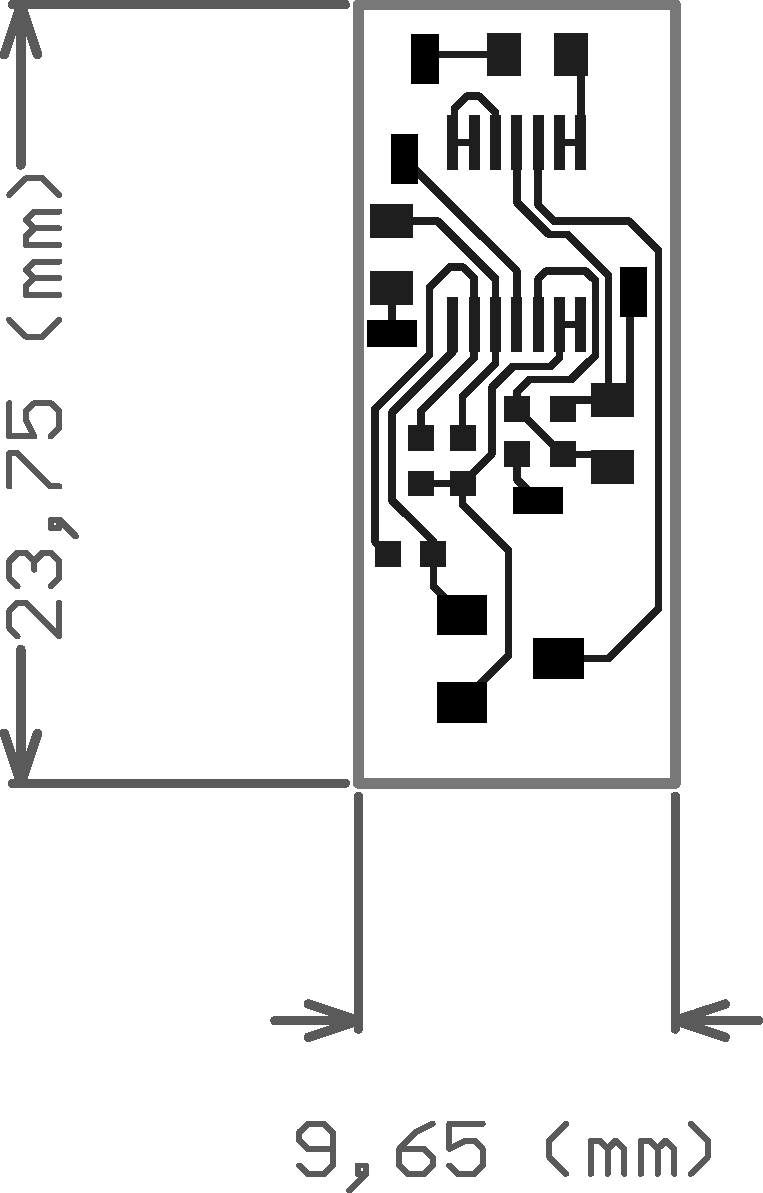
\includegraphics[width=0.2\textwidth]{PreAmp.pdf}
		\caption{The \gls{preamp} layout}
		\label{fig:preamp_layout}
\end{figure}

In \autoref{app:opamp_impedance} it is measured that $Z_i =$\SI{9.18}{\mega\ohm} which follows the assumption, but $Z_o$ is measured to \SI{9.06}{\kilo\ohm} which means that $R_V$ might have to be changed. 
 
\section{Description of the chosen DSP}

The chosen DSP is the Texas Instruments TMS320C5515 Fixed-Point Digital Signal Processor.

\subsection{Power}

The DSP processor gets its power from the \gls{usb} connection.

\subsection{Different Ports}

The C5515 features multiple ports and connectors. It has a micro SD connector, an expansion edge connector as well as a two \gls{usb}s. It also has an audio IN and two Bluetooth interfaces. \\

Each USB connector has a different role, one is used for software purposes and the other one to connect to the personal computer. 

\subsection{LCD Screen}

The \gls{dsp} processor has also an LCD screen that can print different characters by using a string of 14 pins. 

\subsection{Interface with the User}

The processor contains two switch buttons that can be integrated in the software to create an action. 

\subsection{Expansion}

The expansion connectors can be used to redirect the signals to other user interfaces that can be attached to some of the pins on the DSP. The exact number of the pins is in the data sheet. 

\subsection{Monitoring and Testing}

Several "Test points" are available in order to see the signals' behavior moving in the \gls{dsp} processor.

\subsection{Performance}

The \gls{dsp} can run on different speeds depending on how much the \gls{cpu} is powered. The clock rate can be between 60 and 75 MHz if powered with 1.05 Volts and between 100 and 120 MHz if powered with 1.3 Volts. \\

\subsection{Memory}

The chosen DSP has 320 \gls{kb} of \gls{ram} and 120 \gls{kb} of \gls{rom}. \\
There is also a 64 \gls{kb} of dual-access \gls{ram}, 256 \gls{kb} single-access \gls{ram} and 128 single access \gls{rom}. \\
Dual-access and single access \gls{ram}s presented above can be accessed using an internal program, data or \gls{dma} buses. \\
Dual-access and single access \gls{ram}s are divided into blocks that can be accessed using byte address ranges. Ranges are defined for each block but all blocks of a same memory type can be regrouped into one address range. \\
\gls{dma} address range for the block 0 of the dual-access \gls{ram} is 0001 0000h – 0001 1FFFh for instance. \\
All of the addresses are presented in the data sheet tables 2-2, 2-3.
The single-access \gls{rom} is also divided into blocks and has an address range. The usable range can be changed using a software. \\

The external memory interface permits a connection to other memories from other devices than the \gls{dsp}. 
\chapter{\gls{dsp} initializing}
\label{ch:disinit}
In this chapter the \gls{dsp} initializing will be designed. This include \gls{adc}, \gls{dac} and sound in and out. All the \gls{dsp} initializing will be written C and the audio in and out will be written in assembly. 

\section{Sample frequency}
In this section the sample frequency will be designed and initialized to the \gls{dsp} in C. 
%From http://www.ti.com.cn/cn/lit/ml/slaa557/slaa557.pdf 
the necessary reset is done as following \autoref{code:dsp_reset}

\includeCode{aic3204_init.c}{c}{12}{13}{The \gls{adc}/\gls{dac} reset code}{code:dsp_reset}{code/design/}

The necessary initializing for the sample frequency can be derived as \autoref{code:dsp_init}

\includeCode{aic3204_init.c}{c}{22}{13}{The \gls{adc}/\gls{dac} reset code}{code:dsp_init}{code/design/}

\autoref{} can be derived  


\begin{equation}\label{eq:reverb_defined_tal}
       T = \frac{60}{-20 \cdot log10(0.708)} \cdot \tau
       \addunit{\si{\second}}
    \end{equation}

\chapter{Design of Effects}
\section{Design of the Delay and \gls{reverb} Effect}
In this section, the delay and the \gls{reverb} will be designed to fit intro a \gls{dsp}, which mean that a discreet block diagram is obtained and afterwords the equation to the implementation is made. Afterwords the assembly code is developed and implemented. 


\subsection{Obtaining the Differential Equation}
The Delay and \gls{reverb} effect are very similar in their design so they will be presented and designed in the same section. The block diagram presented in \autoref{} is changed so it fit intro a direct form 1 construction. This effect both have \gls{iir} filter and \gls{fir} filter, but it is only the \gls{iir} filter which make the echo, the \gls{fir} filter is only applied to make a flat frequency respond. To get a naturally \gls{reverb} effect with flat amplitude-frequency respond and avoiding fluttering, all the \gls{iir} filters needs to be an all pass filter. The \gls{reverb} needs to have at least 1000 echo per second, and the best way to make as many echo as required, each all pass filter needs to be in serial otherwise if the all pass filter was in parallel, it will require forty all pass filter to make 1000 echo per second \citep{natural_sounding_revorb}. The block diagram in direct form 1 in time domain for the delay and \gls{reverb} effect can be obtained and is shown in \autoref{fig:reverb_block_des}. The \gls{reverb} effect is the one in red and black while the delay is only in black. 

\newpage

\begin{figure} [htbp]
 \centering
\begin{picture}(0,0)%
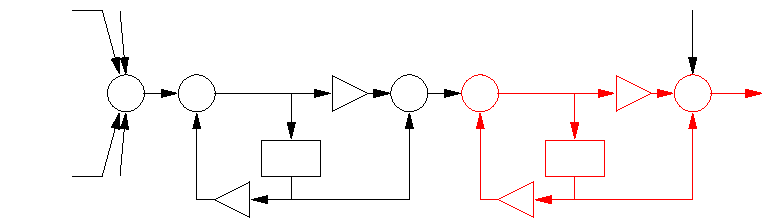
\includegraphics{reverb_diag_des.pdf}%
\end{picture}%
\setlength{\unitlength}{3750sp}%
%
\begingroup\makeatletter\ifx\SetFigFont\undefined%
\gdef\SetFigFont#1#2#3#4#5{%
  \reset@font\fontsize{#1}{#2pt}%
  \fontfamily{#3}\fontseries{#4}\fontshape{#5}%
  \selectfont}%
\fi\endgroup%
\begin{picture}(6927,1683)(-914,-1723)
\put(-135,-409){\makebox(0,0)[lb]{\smash{{\SetFigFont{10}{13.2}{\rmdefault}{\mddefault}{\updefault}{\color[rgb]{0,0,0}-$\alpha$}%
}}}}
\put(-673,-1185){\color[rgb]{0,0,0}$z^{-d}$}%
\put(1876,-1186){\color[rgb]{0,0,0}$z^{-d}$}%
\put(2626,-1186){\color[rgb]{1,0,0}$z^{-d}$}%
\put(3826,-436){\color[rgb]{1,0,0}$\Sigma$}%
\put(1126,-436){\color[rgb]{0,0,0}$\Sigma$}%
\put(526,-436){\color[rgb]{0,0,0}$\Sigma$}%
\put(5126,-1616){\makebox(0,0)[lb]{\smash{{\SetFigFont{10}{13.2}{\rmdefault}{\mddefault}{\updefault}{\color[rgb]{1,0,0}$\alpha$}%
}}}}
\put(5326,-1186){\color[rgb]{1,0,0}$z^{-d}$}%
\put(4426,-436){\color[rgb]{1,0,0}$\Sigma$}%
\put(-899,-286){\color[rgb]{0,0,0}$x[n]$}%
\put(5776,-286){\color[rgb]{1,0,0}$y[n]$}%
\put(1876,-211){\color[rgb]{1,0,0}\textit{Multiply times}}%
\put(1663,-1610){\makebox(0,0)[lb]{\smash{{\SetFigFont{10}{13.2}{\rmdefault}{\mddefault}{\updefault}{\color[rgb]{0,0,0}$\alpha$}%
}}}}
\put(3165,-408){\makebox(0,0)[lb]{\smash{{\SetFigFont{10}{13.2}{\rmdefault}{\mddefault}{\updefault}{\color[rgb]{1,0,0}-$\alpha$}%
}}}}
\end{picture}%
  \caption{The figure shows a block diagram of a \gls{reverb} unit.}
  \label{fig:reverb_block_des}
\end{figure}

From \autoref{fig:reverb_block_des}, the following differential equations can be inferred:

The equation for the delay can be written as:
\begin{equation}
\label{eq:delay_eq}
		y[n] = - \alpha \cdot x[n] + x[n-d] + \alpha \cdot y[n-d]
\end{equation}

Form \citep{natural_sounding_revorb} the \gls{reverb} time is defined by \autoref{eq:reverb_defined}

\begin{equation}
\label{eq:reverb_defined}
		T = \frac{60}{-20 \cdot log(\alpha)} \cdot \tau
\end{equation}

    \startexplain
\explain{$60$ is the \gls{reverb} attenuation in \si{\decibel}, and the \gls{reverb} time is defined that a given signal is attenuated by 60 \si{\decibel}}{\si{\decibel}}

\explain{$\tau$ is the delay over the sample frequency $\tau = \frac{d}{f_s}$}{\si{\second}}

\explain{$T$ is the resulting \gls{reverb} time}{\si{\second}}

\explain{$-20 \cdot log10(\alpha)$ is the attenuation in the feedback loop for each round}{\si{\decibel}}
    \stopexplain

The gain $\alpha$ is is chosen to be 0.708 like useal \gls{reverb} unit  \citep{natural_sounding_revorb} and the total \gls{reverb} echo density shall at lest be 1000 echo per second. In formula \autoref{eq:reverb_defined_tal_res} it can be obtain that $\tau$ shall be $\frac{1}{20}$ of $T$


\begin{subequations}
\begin{equation}\label{eq:reverb_defined_tal}
       T = \frac{60}{-20 \cdot log(0.7)} \cdot \tau
       \addunit{\si{\second}}
    \end{equation}
\centering
$\Updownarrow$
\begin{equation}\label{eq:reverb_defined_tal_res}
        \tau = \frac{1}{20} T
        \addunit{\si{\second}}
    \end{equation}
 \end{subequations}

\autoref{eq:reverb_defined_tal_res} then shows that the $\tau$ time is \SI{50}{\milli\second} with a total \gls{reverb} time $T$ of \SI{1}{second}. This achieve an echo density of 20 echo per second, but the \gls{reverb} unit require 1000 echo per second \citep{natural_sounding_revorb}. To achieve 1000 echo per second there needs to be multiply delay unit in serial. To calculate the number of needed \gls{reverb} unit, $n$ symbolize the number of \gls{reverb} unit in \autoref{eq:reverb_needed} 

\begin{equation}
\label{eq:reverb_needed}
		\frac{1}{\tau} \cdot k^{n-1} \geq  1000
\end{equation}

    \startexplain
\explain{$\tau$ is the delay over the sample frequency $\tau = \frac{d}{f_s}$}{\si{\second}}
\explain{$k$ is the scaling factor, which normally is a factor of tree \citep{natural_sounding_revorb}}{\si{1}}
\explain{$n$ is the required number of \gls{reverb} unit}{\si{1}}
    \stopexplain

The \autoref{eq:reverb_needed}  can be rewritten to \autoref{eq:reverb_needed_mellem}


\begin{subequations}
\begin{equation}\label{eq:reverb_needed_solve}
		\frac{1}{\SI{50}{\milli\second}} \cdot 3^{n-1} \geq  1000
    \end{equation}
\centering
$\Updownarrow$
\begin{equation}\label{eq:reverb_defined_tal_mellem}
        n \geq  \frac{ln(3)+ln{1000 \cdot T}}{ln(3)}
        \addunit{\si{\second}}
    \end{equation}
    $\Updownarrow$
\begin{equation}\label{eq:reverb_defined_tal_res}
        n \geq  4.56
        \addunit{\si{\second}}
    \end{equation}
 \end{subequations}

Since the number of the \gls{reverb} unit only can be integer, the needed numbers of \gls{reverb} unit is 5.

%
%The equation for the \gls{reverb} can be written as:
%
%\begin{equation}
%\label{eq:reverb_eq}
%		y[n] = - \alpha \cdot x[n] + x[n-d] + \alpha \cdot y[n-d]
%\end{equation}

%The index $i$ represents the number of delays that are being implemented in the chorus effect which is also the chorus size. Index $n$ represents the number of samples that are being modulated. \\
%If the implementation is done using a time varying delay, equations \ref{flang_eq} and \ref{chor_eq} can be re-written as:
%
%\begin{equation}
%\label{flang_eq2}
%y[n] = x[n] + x[n- d_{1}[n]] \cdot g_{1}  
%\end{equation}
%
%\begin{equation}
%\label{chor_eq2}
%y[n] = x[n] + \sum_{j=1}^{i}  (x[n- d_{j}[n]] \cdot g_{j})
%\end{equation}
%
%The delay value has to be a periodic function that is varying in a user-defined range. 
%
%\subsection{Matlab Simulation}
%
%A delay can be done in different ways digitally. One way is to use a ring buffer also known as circular buffer. \\
%The idea of this data structure is that it takes values and only outputs them when it gets full, and overwrites the oldest after outputting it. It is a kind of a FIFO queue structure but where the start and the overwriting can start at any index. \\
%This means that the size of the buffer depends on the delay.  The buffer size must then be always up-to-date with the new delay value. \\ 
%The value of the delay is determined by a periodic function as said before, different waveforms can be used as said in \autoref{chor_flang}. A common periodic function that can be used is the sine. Since it varies between 0 and 1, it can be then multiplied with the user-defined range. 
%The delay can then be written as:
%
%\begin{equation}
%	d[n]= A \cdot sin(2\pi f_{l} n)
%\end{equation}
%
%$A$ is the value of the user-defined range which is also the depth. $f_{l}$ is the frequency of the LFO. 
%
%The Matlab code for the flanger effect is:
%
%\begin{lstlisting}[language=Matlab, caption= Matlab code for flanger effect]
%
%%Flanger Effect
%%Group 641
%
%%insert your input in this table
%input = [1 2 3 4 5 6 7 8 9 10]
%
%fs = 1;  %LFO Frequency
%sample_no = length(input) %Length of the input
%g = 0.4; %Gain
%after_delay = (1:1:sample_no); 
%before_delay = (1:1:sample_no);
%output = (1:1:sample_no);
%
%for n = 1:1:sample_no
%	delay = 3 * cos((2*pi*fs)/n);  %Calculate time varying delay
%	buffer = zeros(1,abs(round(delay)));
%
%	for i = 1:1:sample_no %loop for an output with one delay value
%		buffer = [buffer(2:end) input(i)];
%		after_delay(i) = buffer(1) * g;
%		before_delay(i) = input(i); 
%		output(i) = after_delay(i) + before_delay(i);
%	end
%	output
%end
%
%plot(output)
%hold on
%grid
%plot(before_delay)
%
%\end{lstlisting}
%
%
%
%
%

\section{Design of the Chorus and Flanger Effect}

\subsection{Obtaining the Differential Equation}

The flanger- and chorus- effect are similar in their design so they will be presented in the same section. \\

From the block diagram presented in section \autoref{sec:chorus}, a block diagram in the discrete time domain for the flanger and chorus effect can be obtained and is shown in \autoref{fig:chorus_diag_des}. \\ 
The chorus effect is the one in red and black while the flanger is only in black.  
\begin{figure} [htbp!]
	\centering
\begin{picture}(0,0)%
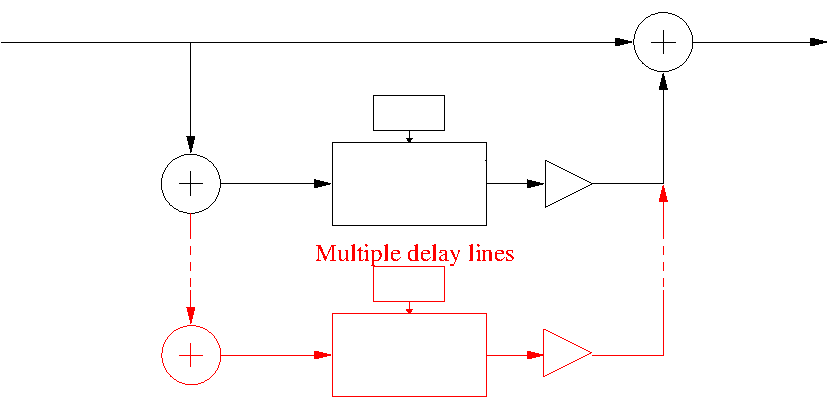
\includegraphics{chorus_diag_des.pdf}%
\end{picture}%
\setlength{\unitlength}{4144sp}%
%
\begingroup\makeatletter\ifx\SetFigFont\undefined%
\gdef\SetFigFont#1#2#3#4#5{%
	\reset@font\fontsize{#1}{#2pt}%
	\fontfamily{#3}\fontseries{#4}\fontshape{#5}%
	\selectfont}%
\fi\endgroup%
\begin{picture}(6327,3018)(3766,-3493)
\put(6571,-1906){\color[rgb]{0,0,0}$z^{-d_{1}}$}%

\put(8101,-1636){\color[rgb]{0,0,0}$g_{1}$}%

\put(6616,-3211){\color[rgb]{1,0,0}$z^{-d_{2}}$}%

\put(8101,-2986){\color[rgb]{1,0,0}$g_{2}$}%

\put(6706,-2671){\color[rgb]{1,0,0}\textit{LFO}}%

\put(6706,-1366){\color[rgb]{0,0,0}\textit{LFO}}%

\put(3781,-646){\color[rgb]{0,0,0}\textit{x[n]}}%

\put(9406,-646){\color[rgb]{0,0,0}\textit{y[n]}}%

\end{picture}%
\caption{Block Diagram of the chorus and flanger effect in the discrete time domain.}
\label{fig:chorus_diag_des}
\end{figure}

From \autoref{fig:chorus_diag_des}, the following differential equations can be inferred:

The equation for the flanger can be written as in \autoref{eq:flang_eq}
\begin{equation}
\label{eq:flang_eq}
		y[n] = x[n] + x[n- d_{1}] \cdot g_{1}  
\end{equation}

The equation for the chorus can be written as in \autoref{eq:chor_eq}:

\begin{equation}
\label{eq:chor_eq}
y[n] = x[n] + \sum_{j=1}^{i}  (x[n- d_{j}] \cdot g_{j})
\end{equation}

The index $i$ represents the number of delays that are being implemented in the chorus effect which is also the chorus size. Index $n$ represents the present sample. \\
If the implementation is done using a time varying delay, equations \ref{flang_eq} and \ref{chor_eq} can be re-written as \autoref{eq:flang_eq2} and \autoref{eq:chor_eq2}:

\begin{equation}
\label{eq:flang_eq2}
y[n] = x[n] + x[n- d_{1}[n]] \cdot g_{1}  
\end{equation}

\begin{equation}
\label{eq:chor_eq2}
y[n] = x[n] + \sum_{j=1}^{i}  (x[n- d_{j}[n]] \cdot g_{j})
\end{equation}

The delay value has to be a periodic function that is varying in a user-defined range. As illustrated in \autoref{fig:chorus_diag_des}, this varying delay can be made from a \gls{lfo}.

The LFO that makes the delay varies is a sine wave in the chorus and the flanger effect. In the case of the flanger, the user can set the LFO frequency between 0,1 and 10 Hz and only the boundaries for the chorus. \\

The gain for the flanger effect can be chosen by the user. For the chorus, the user can choose the boundaries of the gain value that will be randomly selected for each of the delay lines. \\

The number of delay lines for the chorus effect is also a choice but should not exceed 4, the reason is that after 4 lines it has been found that the effect has a strange sound. \\

The delay time for the flanging effect should be between 1 and 20 ms while the delay time in the chorus should be longer than 20ms. \\

From the difference equation, it can be seen that the design is using a FIR Comb filter but where the delay value varies. \todo[inline]{Why is it FIR comb filter?}

\subsection{Making the LFO by Cordic algorithm}
The \gls{lfo} in both the chorus- and the flanger- effect should, as stated in \autoref{}, be able to make sine waves from \SI{0.1}{\kilo\hertz} to \SI{10}{\kilo\hertz}. A \gls{dsp} is not necessarily able to calculate sine values and therefore an algorithm has to be implemented in order to make this possible. A way to do this is by using the \gls{cordic} algorithm, which can be used to calculate both sine, cosine, square roots etc \citep{cordic}. 
When using the \gls{cordic} algorithm for for an \gls{lfo} the two equations \autoref{eq:cordic_x} and \autoref{eq:cordic_y} are almost all what is needed.

\begin{equation}
\label{eq:cordic_x}
		x_{n+1} = x_n \cdot \cos(\theta) - y_n \cdot \cdot \sin(\theta) 
\end{equation}
\startexplain
     \explain{$x_{n+1}$ is the present cosine value.}{\si{1}}
     \explain{$x_n$ is the previous cosine value.}{\si{1}}
     \explain{$y_n$ is the previous sine value.}{\si{1}}
     \explain{$yn$ is the index.}{\si{1}}
    \stopexplain 

\begin{equation}
\label{eq:cordic_y}
		y_{n+1} = y_n \cdot \cos(\theta) + x_n \cdot \sin(\theta) 
\end{equation}
\startexplain
     \explain{$y_{n+1}$ is the present sine value.}{\si{1}}
\stopexplain

The algorithm works by initializing $x_0$ to 1 and $y_0$ to 0. This way $x_1$ becomes equal to $\cos(\theta)$ and $y_1$ becomes equal to $\sin(\theta)$. When the next iteration begins, the initial vector will then have the coordinates [$x_1$, $y_1$]. This way $x_2$ becomes equal to $\cos(2 \cdot \theta)$ and $y_2$ becomes equal to $\sin(2 \cdot \theta)$. Thus it is only necessary to calculate $\cos(\theta)$ and $\sin(\theta)$ and then follow the iterations to produce a sine wave. The frequency of the sine wave is decided by $\theta$. The relation between the frequency and $\theta$ is shown in \autoref{eq:cordic_freq}.

\begin{equation}
\label{eq:cordic_freq}
		\theta = 2 \cdot \pi \cdot \frac{F}{F_s} 
\end{equation}
\startexplain
     \explain{$F$ is the wanted frequency of the sine wave.}{\si{\hertz}}
     \explain{$F_s$ is the sampling frequency.}{\si{\hertz}}
\stopexplain 

This way the \gls{cordic} algorithm will have $\frac{F_s}{F}$ steps round the unitcircle and thereby produce a sine wave with frequency $F$ and sine values between $\pm$1.
A MATLAB simulation of the \gls{cordic} algorithm was made and set to produce a \SI{10}{\hertz} sine wave. The result of the simulation is shown in \autoref{}.

\begin{figure}[!h]
    \centering
        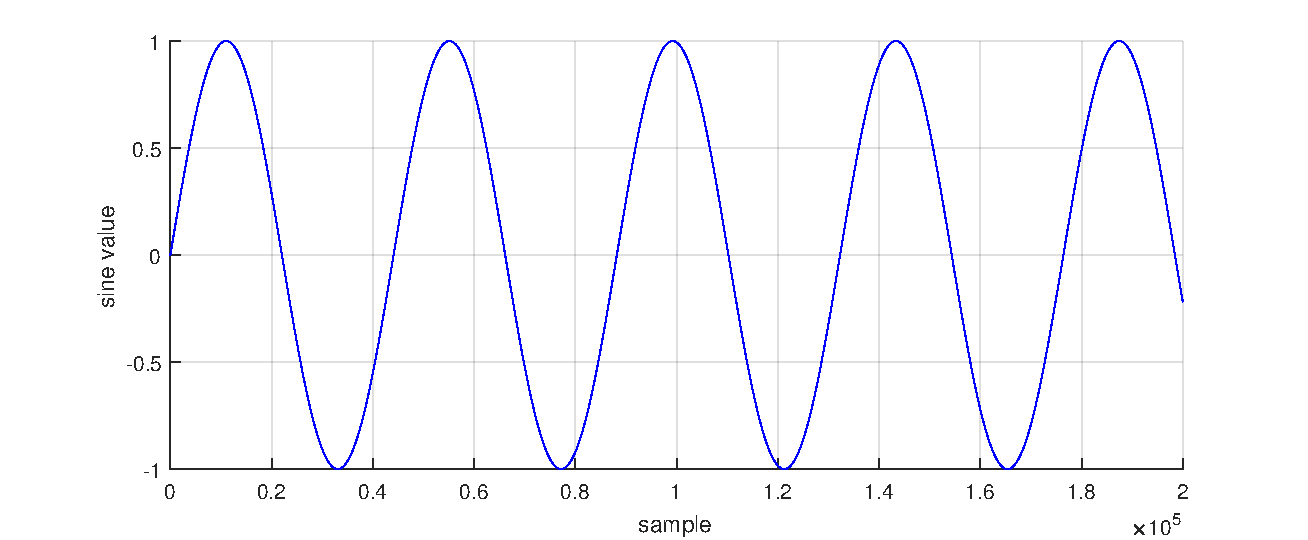
\includegraphics[width=0.5\textwidth]{cordic_1Hz.pdf}
        \caption{Simulation of the \gls{cordic} algorithm, set to produce a \SI{10}{\hertz} sine wave.}
        \label{fig:cordic_10Hz}
  \end{figure}
  
When implementing the \gls{cordic} algorithm on a \gls{dsp}, a gain value smaller than 1, might have to be implemented in \autoref{eq:cordic_x} and \autoref{eq:cordic_y} on $x_n$ and $y_n$ to make the algorithm stable. 







\subsection{Matlab Simulation}

A delay can be done in different ways digitally. One way is to use a ring buffer also known as circular buffer. \\
The idea of this data structure is that it takes values and only outputs them when it gets full, and overwrites the oldest after outputting it. It is a kind of a FIFO queue structure but where the start and the overwriting can start at any index. \\
This means that the size of the buffer depends on the delay.  The buffer size must then be always up-to-date with the new delay value. \\ 
The value of the delay is determined by a periodic function as said before, different waveforms can be used as said in \autoref{chor_flang}. A common periodic function that can be used is the sine. Since it varies between 0 and 1, it can be then multiplied with the user-defined range. 
The delay can then be written as:

\begin{equation}
	d[n]= A \cdot sin(2\pi  \cdot \frac{f_{l}}{f_{s}} n)
\end{equation}

\startexplain
     \explain{$A$ is the value of the user-defined range which is also the depth.}{\si{1}}
     \explain{$f_{s}$ the sampling frequency.}{\si{\hertz}}
     \explain{$f_{l}$ is the frequency of the \gls{lfo}.}{\si{\hertz}}
    \stopexplain 

The Matlab code for the flanger effect is:

\begin{lstlisting}[language=Matlab, caption= Matlab code for flanger effect]

%Flanger Effect
%Group 641
%Mohamed Gabr, Jonas and Sebastian


filename = 'inputttt.wav'; 
%The filename is inserted here, should be in the same directory as the
%codefile.
[input, fs] = audioread(filename, 'native');
%input samples and sample rate are extracted from the file.
input = input / (max(abs(input)));
%the input is rescaled in order to have values between -1 and 1. 
fl = 100;  
%LFO Frequency is chosen here.
sample_no = length(input); 
%Length of the input samples table.
g = 100; 
%Gain
delay_s = 0.0050; 
% The maximum delay in seconds.
after_delay = (1:1:sample_no); 
before_delay = (1:1:sample_no);
output = (1:1:sample_no);
%Needed tables in the code are intialized to make the code faster.
disp('max delay')
max_delay = delay_s * fs  
%Convert the maximum delay from delay in seconds to delay in samples.

buffer = zeros(1,abs(round(max_delay))); 
%intializing the buffer array.

for i = 1:1:sample_no  %Loop that treats a sample per iteration. 
 delay = max_delay * cos(2*pi*i*(fl/fs)); %Calculate time varying delay 
 %(unit is samples)
 buffer = [buffer(2:end) input(i)]; 
 %move the values in the buffer ==> first value overwritten, one new 
 %value added at the end.
 if abs(delay) < 1   %All delay values less than zero are considered as
  %not having a delay
  after_delay(i) = 0;
 else
  if floor(delay) == delay || abs(floor(delay)) >= floor(max_delay)
   after_delay(i) = buffer(round(abs(delay))) * g;
   %Treating the case when the delay is an integer and when it has a
   %value bigger than the maximum delay. 
  else %Treating the case when the delay is not an integer
   x1 = abs(floor(delay));
   x2 = x1 + 1;
   y1 = buffer(x1);
   y2 = buffer(x2);
   coeff = (y1 - y2)/(x1 - x2);
   %Making a linear approximation between the samples to increase
   %precision
   after_delay(i) = delay * coeff * g;  %sound from the delay line
   %in the block diagram 
  end
 end
 before_delay(i) = input(i);  %sound from the direct line
 output(i) = after_delay(i) + before_delay(i); %output delayed signal 
end
output = output / max(abs(output)); %output is rescaled to values between
% -1 and 1 to avoid clipping. 
audiowrite('out_flan.wav',output,fs); %Writing the values in a file, 
% PS: audiowrite will clip if the values are not between -1 and 1. 
plot(output,'r') %plotting the output samples in red.
hold on
grid
plot(before_delay,'b') %plotting the input samples in blue on the same fig.




\end{lstlisting}


The code is commented for the user's instruction.\\

The Matlab code for the chorus effect is:

\begin{lstlisting}[language=Matlab, caption= Matlab code for chorus effect]

%Chorus Effect
%Group 641
%Mohamed, Jonas and Sebastian

filename = 'inputttt.wav'; %Typing the filename, should be in same 
%directory as the codefile
[input, fs] = audioread(filename);
%input samples and sample rate are extracted from the file.
input = input / (max(abs(input)));
%the input is rescaled in order to have values between -1 and 1.
lines = 5; %number of chorus lines 
fl = randi(10,1,lines);
%LFO Frequencies for each line are generated.
delay = (1:1:lines);
%Delay table generated here to speed the coding. 
sample_no = length(input); 
%Length of the input samples
g = rand(1,lines); 
%Gain values generated here
delay_s = 0.025; 
% Maximum delay in seconds 
after_delay = rand(lines, sample_no); 
before_delay = (1:1:sample_no);
output = (1:1:sample_no);
% Generating tables to speed the code. 
max_delay = delay_s * fs  
%convert the delay from delay in seconds to delay in samples. 


buffer = zeros(1,abs(round(max_delay))); %create the buffer array 

for i = 1:1:sample_no %loop that gives one output sample per iteration
 buffer = [buffer(2:end) input(i)]; %moving buffer values
 before_delay(i) = input(i); %Value before delay
 output(i) = before_delay(i); %adding it to one output sample
 for j = 1:1:lines %Generating delays and then samples after delay for 
 %each chorus line
   delay(j) = max_delay * cos(2*pi*i*(fl(j)/fs)); %Calculate time  
   %varying delay (unit is samples)
   if abs(delay(j)) < 1 %Treating the case where the delay is less 
   %than one.
	 after_delay(j,i) =0;
   else
	 if floor(delay(j)) == delay(j) || abs(floor(delay(j))) >= floor(max_delay)
	   after_delay(j,i) = buffer(round(abs(delay(j)))) * g(j);
	   %Treating the case when the delay is an integer and when it has a
	   %value bigger than the maximum delay. 
	 else  %Treating the case when the delay is not an integer
	   x1 = abs(floor(delay(j)));
	   x2 = x1 + 1;
	   y1 = buffer(x1);
	   y2 = buffer(x2);
	   coeff = (y1 - y2)/(x1 - x2);
	   %Making a linear approximation between the samples to increase
	   %precision
	   after_delay(j,i) = delay(j) * coeff * g(j);  
	   %sound from the delay line in the block diagram
	 end
   end
   output(i) = output(i) + after_delay(j,i);
   %Signal output sample
 end
end
output = output / max(abs(output)); %output is rescaled to values between
% -1 and 1 to avoid clipping. 
audiowrite('out_chor.wav',output,fs); %Writing the values in a file, 
% PS: audiowrite will clip if the values are not between -1 and 1.
plot(output,'r') %plotting the output samples in red.
hold on
grid
plot(before_delay,'b') %plotting the input samples in blue on the same fig.



\end{lstlisting}

The codes where simulated on different audiofiles. 



\section{Design of the equalizer}
This chapter aims to describe the design of an digital graphic equalizer, for an electric guitar. By graphic equalizer it is meant that only the gain of each band is changeable for the user.  
To begin with, some design choices have to made. From \autoref{tab:frequency_area} it is seen that the frequency area of an electric guitar is from \SI{80}{\hertz} to \SI{4400}{\hertz}. Thus the equalizer has to be able to change the frequency response in this area. This change in the frequency response is made by a combination of shelving filters and peak filters. The shelving filters are used for the highest and the lowest bands of the equalizer and the peak filters are used for the in between bands. All filters are normally kept as first or second order filters. 

\subsection{Shelving filter}
The transfer function for a first order low shelving filter is as in \autoref{eq:analog_shelving_low} \citep{Julius_smith}.

\begin{equation}\label{eq:analog_shelving_low}
        H_{LS}(s) = G \cdot \frac{\omega_c}{s+\omega_c}
    \end{equation}

    \startexplain
    \explain{$H_{LS}(s)$ is the low shelving filters transfer function.}{\si{1}}
     \explain{$G$ is the gain.}{\si{1}}
	\explain{$\omega_c$ is the transition frequency dividing low and high frequencies.}{\si{\radian/\second}}
    \stopexplain
    
The transfer function for a first order high shelving filter is as in \autoref{eq:analog_shelving_low}.

\begin{equation}\label{eq:analog_shelving_high}
        H_{HS}(s) = G \cdot \frac{s}{s+\omega_c}
    \end{equation}

    \startexplain
    \explain{$H_{HS}(s)$ is the high shelving filters transfer function.}{\si{1}} 
    \stopexplain

    
When implementing \autoref{eq:analog_shelving_low} and \autoref{eq:analog_shelving_high}, individually in a feedforward loop, as in \autoref{fig:shelving_block}, the bodeplots of first order low- and high- shelving filters with different cut-off frequencies, becomes as in \autoref{fig:low_and_high_shelving}.

\begin{figure}[!h]
\centering
\def\svgwidth{0.72\columnwidth}
\scalebox{1}{\input{figures/design/shelving_filter_block.pdf_tex}}
\caption{Block diagram of the shelving filter.}
		\label{fig:shelving_block}
\end{figure}

\begin{figure}
    \centering
        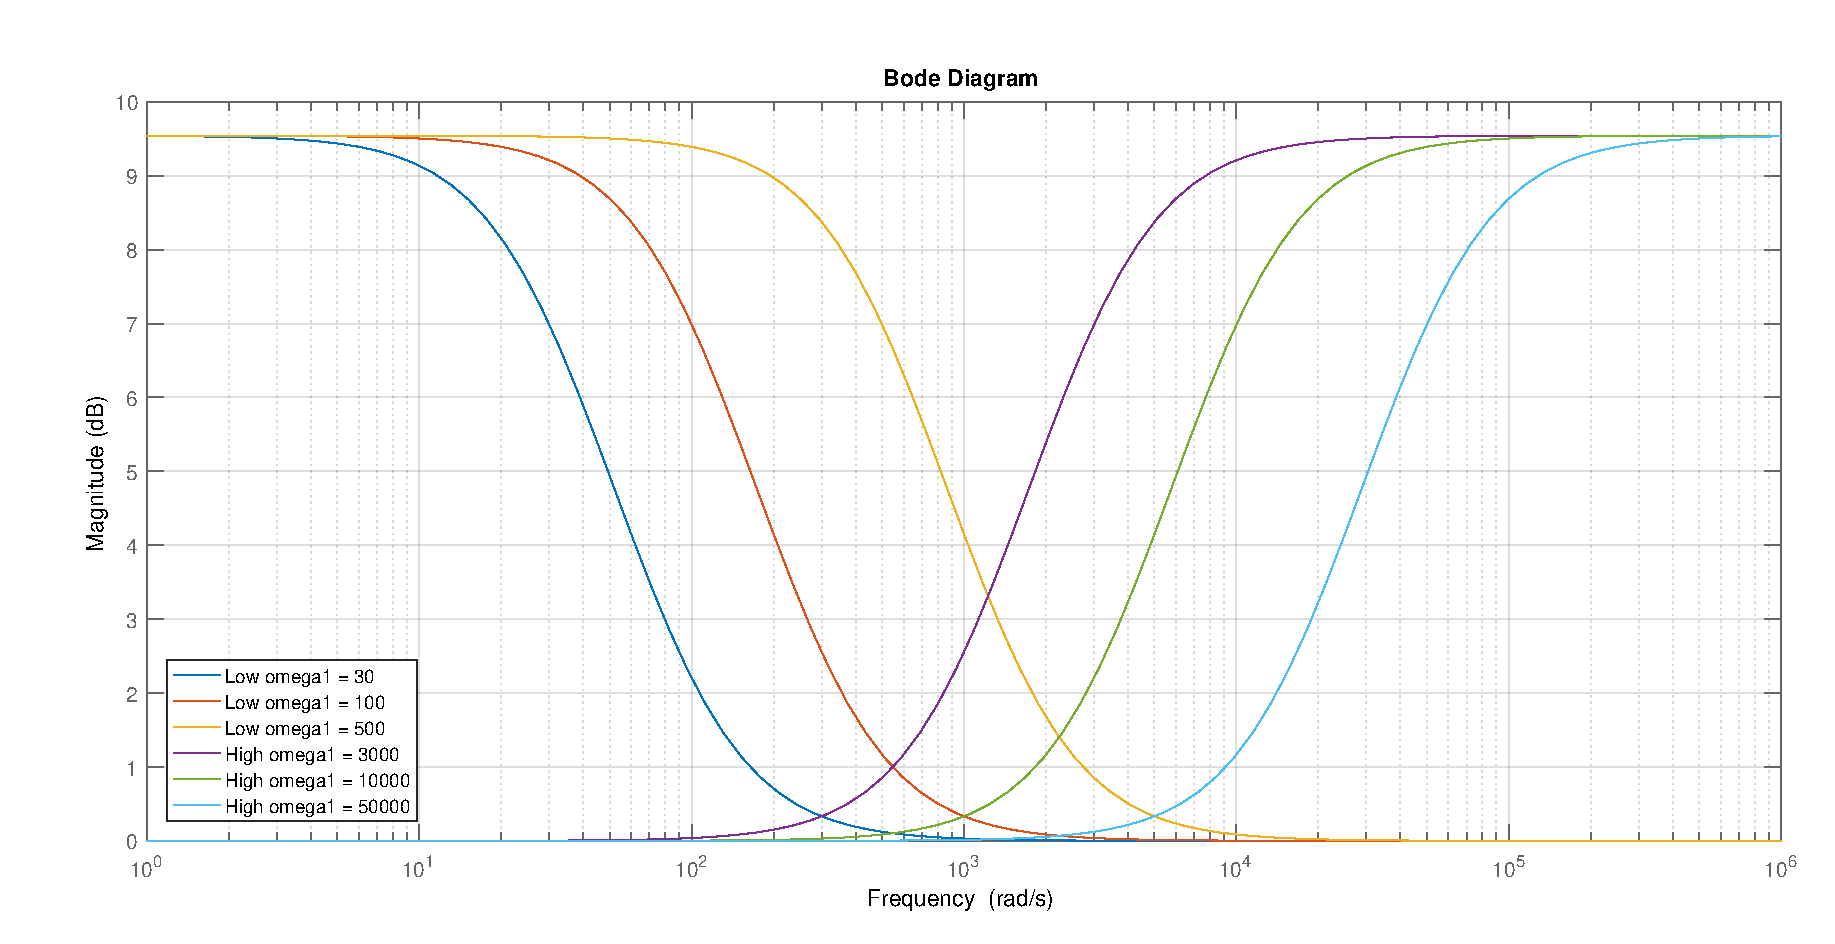
\includegraphics[width=\textwidth]{low_and_high_shelfing.pdf}
        \caption{Bodeplot of first order low- and high- shelving filters with different transition frequencies.}
        \label{fig:low_and_high_shelving}
  \end{figure} 
  %\todo[inline]{figure is now first order}

\subsection{Peak filter}
The peak filters for the in between bands can be made from a number of design topologies. One of these are the constant-Q design. This design is sufficient the way that it keeps a specified bandwidth of the filter and therefore each individual filter's impact on the neighbouring filters can be controlled \citep{constant_Q}.
A way to make these constant-Q peak filters, and keep the order of the filter low, is by combining a second order lowpass filter with a high Q-value, and a linear function in Laplace domain.
The transfer function for the analog second order lowpass filter is as in \autoref{eq:analog_2nd_order_LP} and the transfer function for the analog linear function is as in \autoref{eq:analog_linear_function}. Their bodeplot can be seen in \autoref{fig:lin_function_&_2nd_order_LP}, where $Q = 4$ and $\omega_0 = 1000$. 

\begin{equation}\label{eq:analog_2nd_order_LP}
        H_{LP}(s) = \frac{\omega_0^2}{s^2+\frac{\omega_0}{Q}\cdot s + \omega_0^2}
    \end{equation}

    \startexplain
     \explain{$\omega_0$ is the cut-off frequency.}{\si{\radian/\second}}
     \explain{$Q$ is the ratio between the center frequency and the bandwidth.}{\si{1}}
    \stopexplain

\begin{equation}\label{eq:analog_linear_function}
        H_{lin}(s) = \frac{s}{\omega_0 \cdot Q}
    \end{equation}
    
\begin{figure}
    \centering
        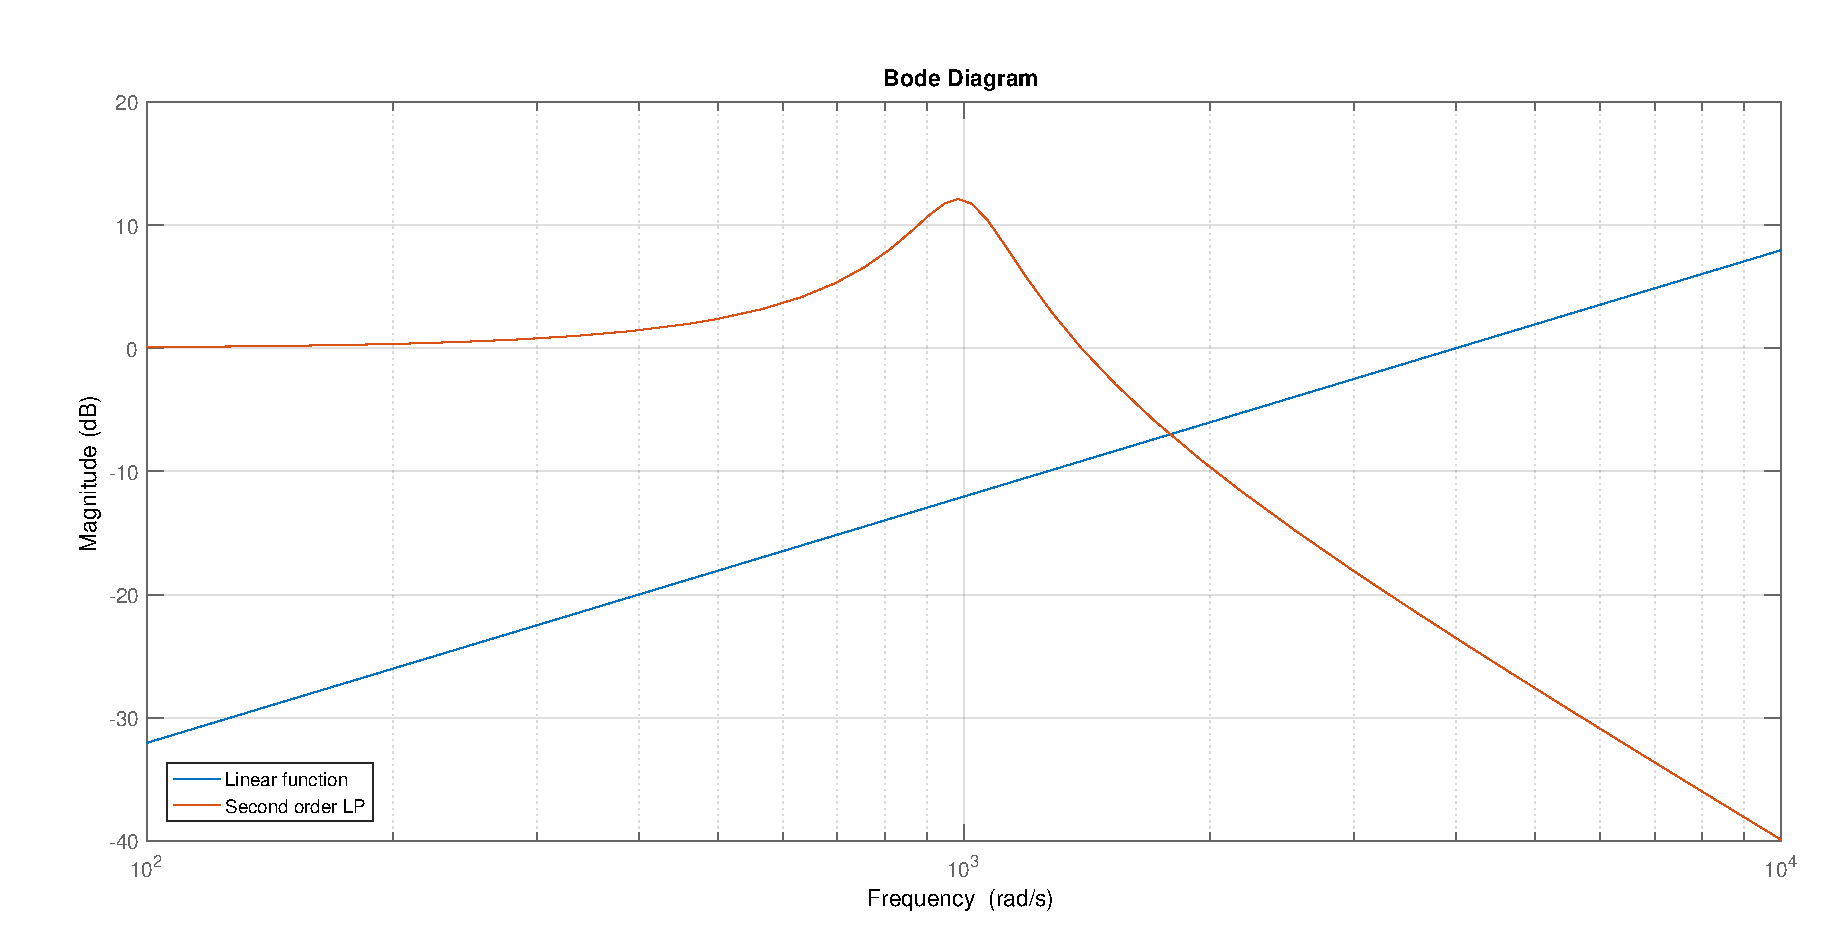
\includegraphics[width=\textwidth]{linear_function_and_2nd_order_LP.pdf}
        \caption{Bodeplot of a linear function and second order lowpass filter.}
        \label{fig:lin_function_&_2nd_order_LP}
  \end{figure} 

To make a peak filter, the two functions in \autoref{fig:lin_function_&_2nd_order_LP} are connected in series to make the analog peak filter transferfuntion as in \autoref{eq:H_peak}.

\begin{equation}\label{eq:H_peak}
        H_{peak}(s) = G \cdot \frac{\frac{\omega_0}{Q}\cdot s}{s^2+\frac{\omega_0}{Q}\cdot s + \omega_0^2}
    \end{equation}
    
    \startexplain
    \explain{$H_{peak}(s)$ the analog transferfunction of the peak filter.}{\si{1}}
     \explain{$G$ is the gain of the peak filter.}{\si{1}}
    \stopexplain

\begin{figure}[!h]
\centering
\def\svgwidth{\columnwidth}
\input{figures/design/peak_filter_block.pdf_tex}
\caption{Block diagram of a peak filter.}
		\label{fig:peak_filter_block}
\end{figure}

When implementing \autoref{eq:H_peak} in a feedforward loop as in \autoref{fig:peak_filter_block}, the bodeplot becomes as in \autoref{fig:peak_filter}, where $Q = 4$, $\omega_0 = 1000$ and various gain values. 



\begin{figure}[!h]
    \centering
        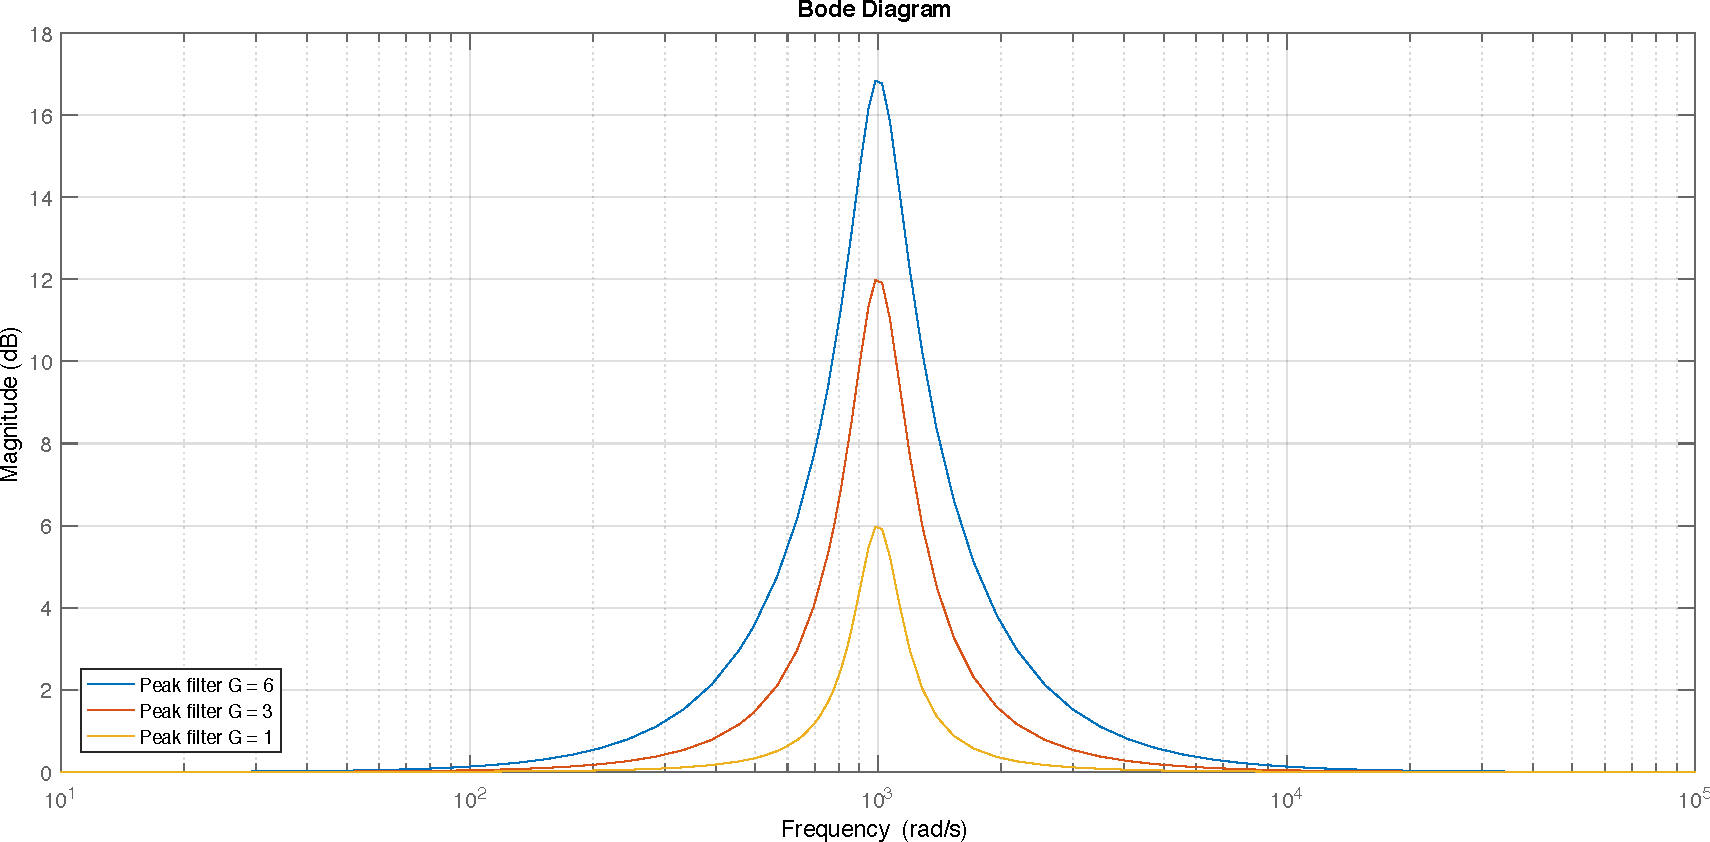
\includegraphics[width=\textwidth]{peak_filter.pdf}
        \caption{Bodeplot of a peak filter with various gain values.}
        \label{fig:peak_filter}
  \end{figure} 
  
\subsection{Design choices and calculation of filter parameters}
All the parts needed to make an equalizer have now been described. The parameters after which the equalizer shall be designed, will now be presented. 
The equalizer will be inspired by the BOSS GE-7 which is an analog equalizer for an electric guitar. The equalizer designed in this report will have the same number of bands and have the same attenuation and amplification ranges as the BOSS GE-7 \citep{Boss_GE7}. Thus the equalizer will have seven bands and be able to amplify each band $\pm$ \SI{15}{\decibel}.
The center frequencies of the seven bands are also inspired by the BOSS GE-7 and is placed as in \autoref{tab:center_frequencies}.

\begin{table}[htbp]
\centering
\caption{Center frequencies for the equalizer.}
\label{tab:center_frequencies}
\begin{tabular}{|l|l|}
\cline{1-2}
\textbf{Band} & \textbf{Center frequency} \\ \cline{1-2}
1st & \SI{100}{\hertz} \\  \cline{1-2}
2nd & \SI{200}{\hertz}\\ \cline{1-2}
3rd & \SI{400}{\hertz} \\ \cline{1-2}
4th & \SI{800}{\hertz} \\ \cline{1-2}
5th & \SI{1600}{\hertz} \\ \cline{1-2}
6th & \SI{3200}{\hertz} \\ \cline{1-2}
7th & \SI{6400}{\hertz} \\ \cline{1-2}
\end{tabular}
\end{table}

The first and the seventh band will be made by shelving filters and band 2,3,4,5 and 6 will be made by peak filters. The aim of the design is to design an equalizer, where each band can be amplified $\pm$ \SI{15}{\decibel} and has a flat combined frequency response when each band is set to amplify \SI{15}{\decibel}.
The individual filters in the amplifying equalizer will coupled in parallel as seen in \autoref{fig:eq_parallel}.

\begin{figure}[!h]
\centering
\def\svgwidth{0.72\columnwidth}
\scalebox{1}{\input{figures/design/eq_parallel.pdf_tex}}
\caption{Block diagram of the combined amplifying equalizer.}
		\label{fig:eq_parallel}
\end{figure}

The shelving filters will be designed first, followed by the peak filters. Since the transition frequencies, $\omega_c$ for the low- filter and high shelving filters, are found in \autoref{tab:center_frequencies}, the only unknown in \autoref{eq:analog_shelving_low} is the gain, $G$.
The gain has to be changeable within $\pm$ \SI{15}{\decibel}. It is chosen that it is the passband that will be amplified \SI{15}{\decibel} and not the transition frequency, $\omega_c$. Thus the shelving filters gain is found by setting $\omega_c =$ \SI{100}{\radian/\second} and then finding the gain for $\omega =$ \SI{1}{\radian/\second}. The gain value for a \SI{15}{\decibel} attenuation is found in \autoref{eq:shelving_gain_value}.

\begin{subequations}
\begin{equation}\label{eq:shelving_gain}
       20 \cdot \log_{10} \left( \mathopen|1 + H_{LS}(j\cdot \omega) \mathclose| \right) = 15 \addunit{\SI{}{\decibel}}
    \end{equation}
 \centering
$\Updownarrow$   
\begin{equation}\label{eq:shelving_gain_value}
       G_{LS-boost} = \frac{\sqrt{(\omega_c^2+\omega^2) \cdot 10^{\frac{12}{10}}-\omega^2}}{\omega_c} - 1 \Big|_{\omega = 1 \ and \ \omega_c = 100} = 4.62 \addunit{\SI{}{1}}
    \end{equation}
\end{subequations}

All parameters in the shelving filters are now known and the peak filters will now be designed.
Since $\omega_0$ is fixed for each band, only $G$ and $Q$ have to be determined. The gain, $G$, has to changeable within $\pm$ \SI{15}{\decibel}.
What the gain should be for the band to amplify \SI{15}{\decibel} is found in \autoref{eq:peak_gain_value}


\begin{subequations}
\begin{equation}\label{eq:peak_gain}
       20 \cdot \log_{10} \left(\mathopen|1 + H_{peak}(j\omega_0)\mathclose|\right) = 20 \cdot \log_{10} \left(1+G_{peak-boost}\right) = 15 \addunit{\SI{}{\decibel}}
    \end{equation}
\centering
$\Updownarrow$
\begin{equation}\label{eq:peak_gain_value}
        G_{peak-boost} = -1+10^{\frac{3}{4}} = 4.62 \addunit{\SI{}{1}}
    \end{equation}
 \end{subequations}
 
 

The Q-value is then the only unknown in the design of the peak filters. In \autoref{req:equalizer2} it is stated that at full amplification (\SI{15}{\decibel}), the amplification at the neighbouring centerfrequencies must drop to (\SI{9}{\decibel}). 
The Q-value will be chosen so it has the minimum ripple. This Q-value is found using a MATLAB program, where the Q-value is increased in steps of 0.2 from 0 to 10. All gains on both the peak and the shelving filters are set to amplify \SI{15}{\decibel}. The optimal Q-value is hereby found to be 1.4, giving a ripple of $\pm$\SI{1.11}{\decibel}, in the frequency area from \SI{100}{\hertz} to \SI{6400}{\hertz}, when all filters are fully amplified. All parameters for the peak filters are then found. 
When coupling the filters as in \autoref{fig:eq_parallel}, and plotting it in MATLAB, the bodeblot of the equalizer with all filters fully amplified, is as in \autoref{fig:eq_s_domain_comb}. In the figure all bands have their maximum gain value.

\begin{figure}[!h]
    \centering
        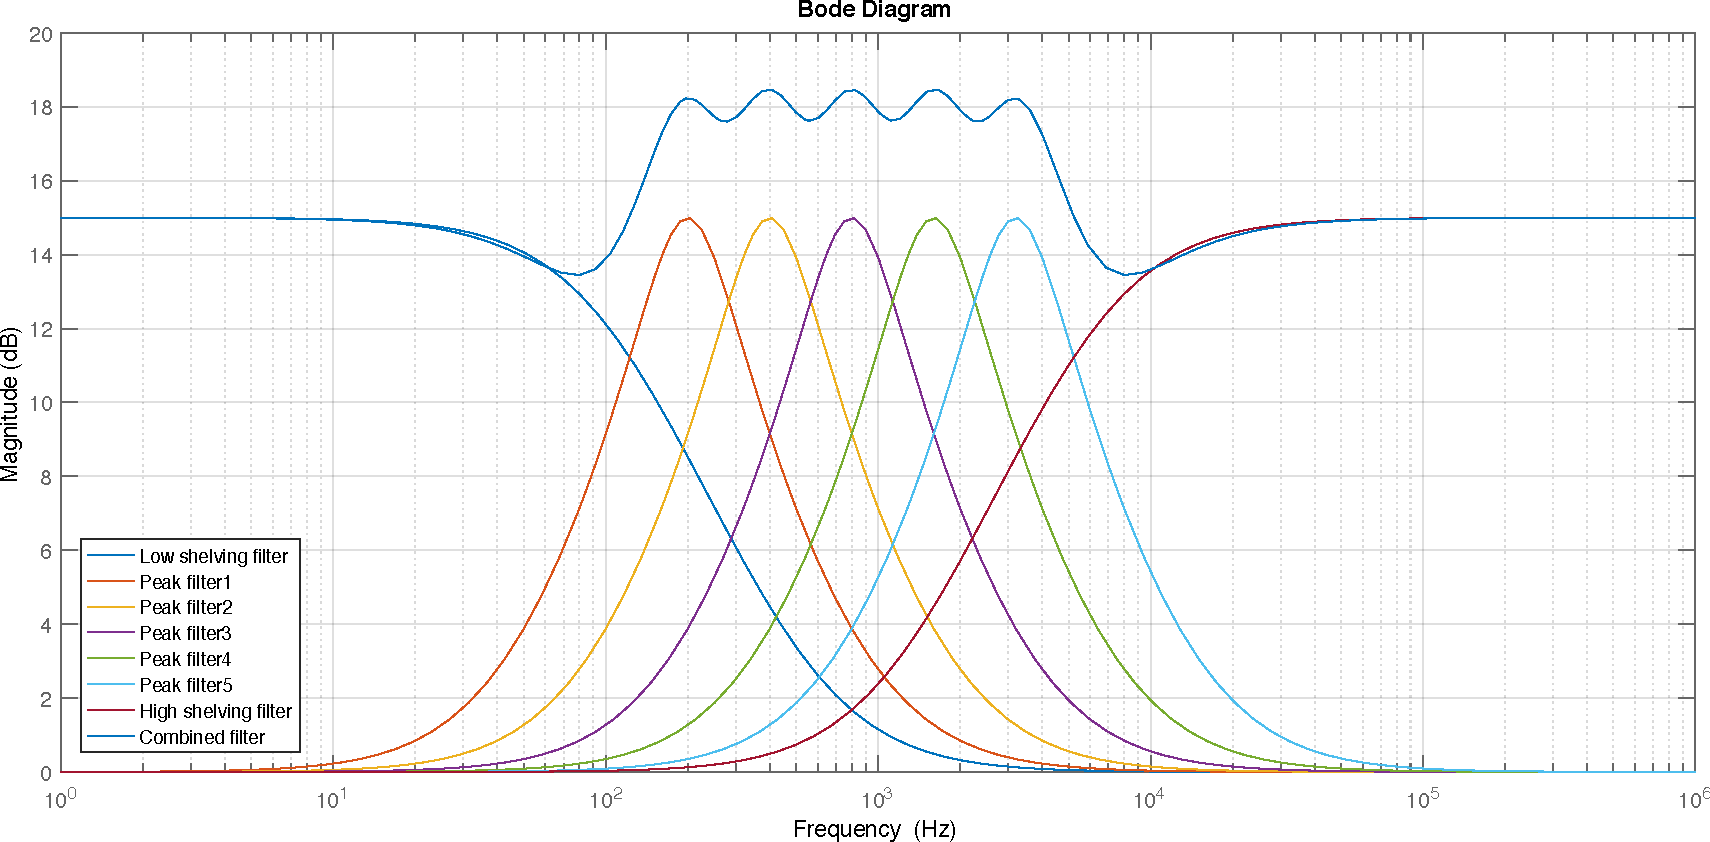
\includegraphics[width=\textwidth]{eq_s_domain_comb.pdf}
        \caption{Bodeplot of the combined equalizer in s-domain, with maximum gain on all bands.}
        \label{fig:eq_s_domain_comb}
  \end{figure}

The ripple of the combined equalizer in s-domain, when all bands are fully amplified, is \SI{4.49}{\decibel}, in the frequency area from \SI{100}{\hertz} to \SI{6400}{\hertz}. This ripple is accepted as a compromise, in order to make each band independent from the neighbouring bands. 

It is chosen that the equalizer shall be able to amplify each band in five different steps from \SI{0}{\decibel} to \SI{15}{\decibel}. Using \autoref{eq:shelving_gain} and \autoref{eq:peak_gain}, and changing the value on the right side of the equality sign, the gain values for the five steps are found. The gain values are shown in \autoref{tab:eq_gain_values}. 

\begin{table}[htbp]
\centering
\caption{Gain values for the equalizer.}
\label{tab:eq_gain_values}
\begin{tabular}{|l|l|l|}
\cline{1-3}
\textbf{Amplification [dB]} & \textbf{Gain value (shelving)} & \textbf{Gain value (peak)} \\ \cline{1-3} 
3 & 0.41 & 0.41 \\  \cline{1-3} 
6 & 0.99 & 0.99 \\ \cline{1-3} 
9 & 1.81 & 1.81 \\ \cline{1-3} 
12 & 2.98 & 2.98 \\ \cline{1-3} 
15 & 4.62 & 4.62 \\ \cline{1-3} 
\end{tabular}
\end{table}

\subsection{Converting the equalizer to z-domain}
In order to implement the equalizer on a \gls{dsp}, the now designed analog equalizer, has be to converted to a digital equalizer. This conversion will be made by using the bilinear transformation, which converts analog filters into digital IIR filters. In \autoref{eq:bilinear_transformation} the bilinear transformation method is shown.

\begin{equation}\label{eq:bilinear_transformation}
        H(z) = H(s) \Big|_{s = \frac{2}{T_s} \cdot \frac{z-1}{z+1}}
    \end{equation}
    
    \startexplain
     \explain{$H(z)$ is the digital transferfunction.}{\si{1}}
     \explain{$T_s$ is the sample time.}{\si{\second}}
    \stopexplain
    
Applying this conversion on the shelving and the peak filters, the digital transferfunctions becomes as in \autoref{eq:Hz_LS}, \autoref{eq:Hz_HS} and \autoref{eq:H_peak}.

\begin{equation}\label{eq:Hz_LS}
        H(z)_{LS} = G \cdot \frac{z \cdot a_{LS1} + a_{LS2}}{z \cdot b_{LS1} + b_{LS2}}
    \end{equation}
    
    \startexplain
     \explain{$H(z)_{LS}$ is the digital transferfunction for the low shelving filter.}{\si{1}}
     \explain{$a_{LS1} = a_{LS2} = \omega_c \cdot T_s$ }{\si{1}}
     \explain{$b_{LS1} = 2+\omega_c \cdot T_s$ }{\si{1}}
     \explain{$b_{LS2} = -2+\omega_c \cdot T_s$ }{\si{1}}
    \stopexplain
    
\begin{equation}\label{eq:Hz_HS}
        H(z)_{HS} = G \cdot \frac{z \cdot a_{HS1} + a_{HS2}}{z \cdot b_{HS1} + b_{HS2}}
    \end{equation}
    
    \startexplain
     \explain{$H(z)_{HS}$ is the digital transferfunction for the high shelving filter.}{\si{1}}
     \explain{$a_{HS1} = 2$ }{\si{1}}
     \explain{$a_{HS2} = -2$ }{\si{1}}
     \explain{$b_{HS1} = 2+\omega_c \cdot T_s$ }{\si{1}}
     \explain{$b_{HS2} = -2+\omega_c \cdot T_s$ }{\si{1}}
    \stopexplain

\begin{equation}\label{eq:Hz_peak}
        H(z)_{peak} = G \cdot \frac{z^2 \cdot a_{peak1} + a_{peak2}}{z^2 \cdot b_{peak1} + z \cdot b_{peak2} + b_{peak3}}
    \end{equation}
    
    \startexplain
     \explain{$H(z)_{peak}$ is the digital transferfunction for the peak filter.}{\si{1}}
     \explain{$a_{peak1} = 2 \cdot \omega_0 \cdot T_s$ }{\si{1}}
     \explain{$a_{peak2} = -2 \cdot \omega_0 \cdot T_s$ }{\si{1}}
     \explain{$b_{peak1} = 4 \cdot Q + 2 \cdot \omega_c \cdot T_s + \omega_0^2 \cdot T_s^2 \cdot Q$ }{\si{1}}
     \explain{$b_{peak2} = -8 \cdot Q + 2 \cdot  \omega_0^2 \cdot T_s^2 \cdot Q$ }{\si{1}}
     \explain{$b_{peak3} = 4 \cdot Q - 2 \cdot \omega_c \cdot T_s + \omega_0^2 \cdot T_s^2 \cdot Q$ }{\si{1}}
    \stopexplain

The combined transferfunction, when combining the transferfunctions as in \autoref{fig:eq_parallel}, becomes as in \autoref{fig:eq_z_domain_comb}.

\begin{equation}\label{eq:z_to_n_final}
        H(z)_{comb} = 1 + H(z)_{LS} + H(z)_{HS} +  \sum_{j=1}^{5} H(z)_{peak(j)}
    \end{equation}

When choosing the sampling frequency, $f_s =$ \SI{44.1}{\kilo \hertz}, and thereby $T_s = \frac{1}{f_s} =$ \SI{22.68}{\micro \second}, setting $Q = 1.4$, and using the frequencies in \autoref{tab:center_frequencies} as $\omega_c$ and $\omega_0$, the frequency response of the digital equalizer, with all bands fully amplified, looks like in \autoref{fig:eq_z_domain_comb}.

\begin{figure}[!h]
    \centering
        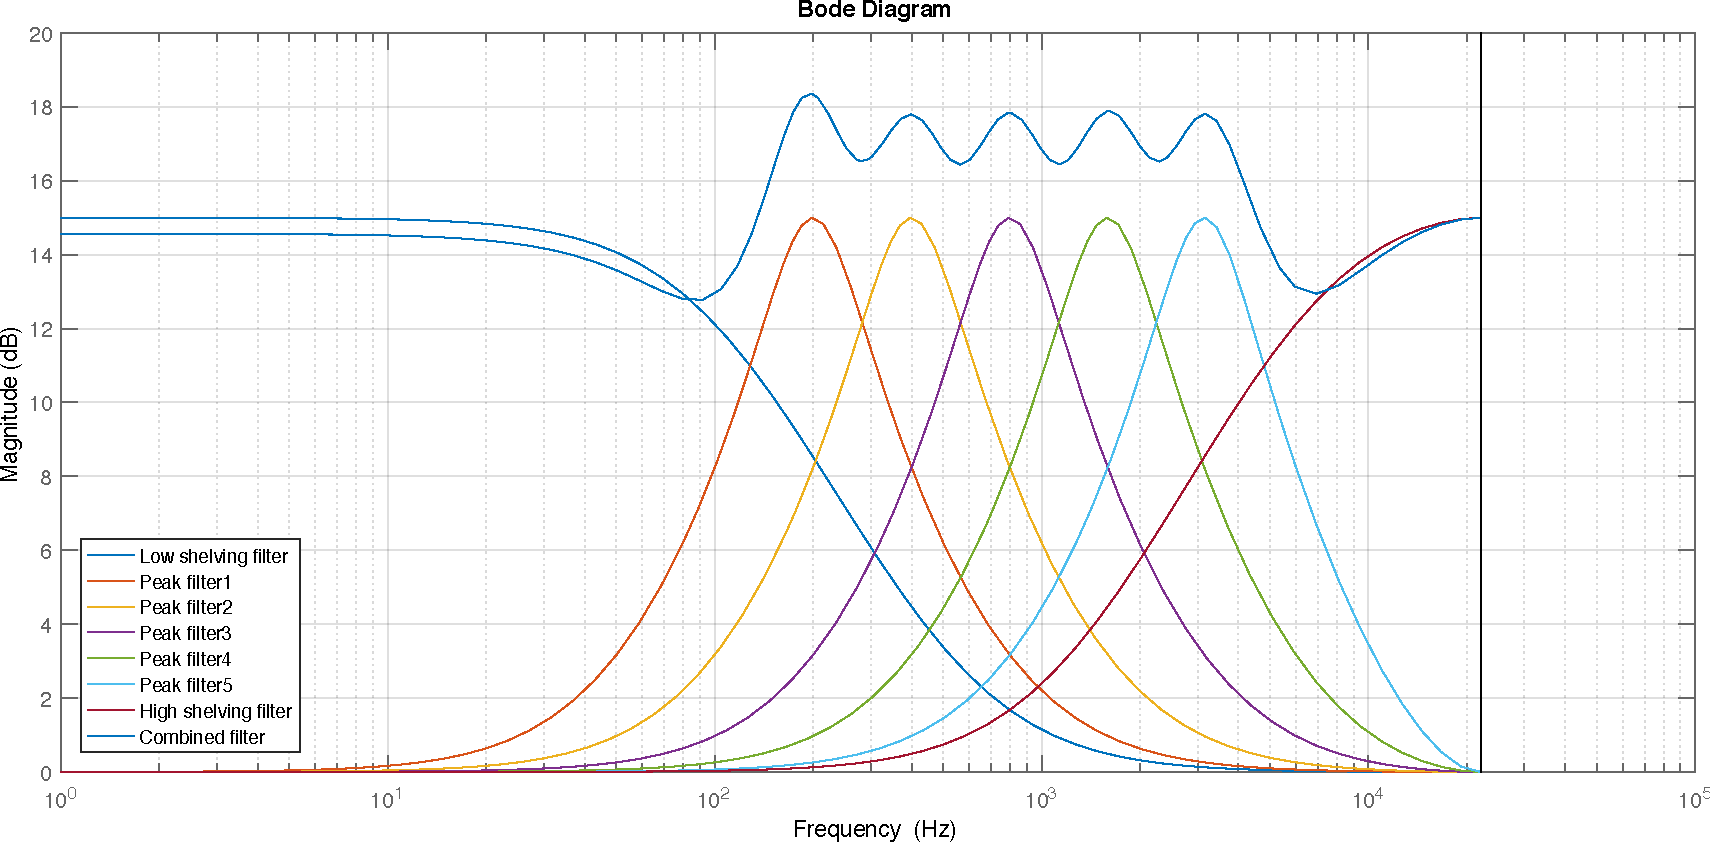
\includegraphics[width=\textwidth]{eq_z_domain_comb.pdf}
        \caption{Bodeplot of the combined equalizer in z-domain, with maximum gain on all bands.}
        \label{fig:eq_z_domain_comb}
  \end{figure}

The conversion is made without prewarping, because the frequency response, when using prewarping, changed in an unwanted way at low frequencies.

\subsection{Converting the equalizer to n-domain}
The last step in making the equalizer implementable in a \gls{dsp}, is to convert the z-domain transferfunction, into a differential equation in n-domain. The procedure of doing this, will be shown for the peak filters, but the procedure is the same for the shelving filters. The conversion from z-domain to n-domain is shown in the equations \autoref{eq:z_to_n1} to \autoref{eq:z_to_n7} 

\begin{subequations}
\begin{equation}\label{eq:z_to_n1}
       H(z)_{peak} = \frac{Y(z)}{X(z)} = G \cdot \frac{z^2 \cdot a_{peak1} + a_{peak2}}{z^2 \cdot b_{peak1} + z \cdot b_{peak2} + b_{peak3}}
    \end{equation}

\begin{equation}\label{eq:z_to_n2}
        \frac{Y(z)}{X(z)} = G \cdot \frac{a_{peak1} + a_{peak2} \cdot z^{-2}}{b_{peak1} + b_{peak2} \cdot z^{-1} + b_{peak3} \cdot z^{-2}}
    \end{equation}
    \centering
$\Updownarrow$
\begin{equation}\label{eq:z_to_n3}
        Y(z) \cdot (b_{peak1} + b_{peak2} \cdot z^{-1} + b_{peak3} \cdot z^{-2}) = X(z) \cdot G \cdot (a_{peak1} + a_{peak2} \cdot z^{-2})
    \end{equation}
       \centering
$\Updownarrow$
\begin{equation}\label{eq:z_to_n4}
         Y(z) \cdot b_{peak1} + Y(z) \cdot b_{peak2} \cdot z^{-1} + Y(z) \cdot b_{peak3} \cdot z^{-2} =  G \cdot (X(z) \cdot a_{peak1} + X(z) \cdot a_{peak2} \cdot z^{-1})
    \end{equation}
    \centering
    $\Downarrow Z^{-1}$
\begin{equation}\label{eq:z_to_n5}
         b_{peak1} \cdot y[n] + b_{peak2} \cdot y[n-1] + b_{peak3} \cdot y[n-2] =  G \cdot (a_{peak1} \cdot x[n] + a_{peak2} \cdot x[n-2])
    \end{equation}
    \centering
    $\Updownarrow$
\begin{equation}\label{eq:z_to_n6}
         b_{peak1} \cdot y[n] =  G \cdot (a_{peak1} \cdot x[n] + a_{peak2} \cdot x[n-2]) -  b_{peak2} \cdot y[n-1] - b_{peak3} \cdot y[n-2]
    \end{equation}
    \centering
    $\Updownarrow$
\begin{equation}\label{eq:z_to_n7}
         y_{peak}[n] = \frac{G \cdot a_{peak1}}{b_{peak1}} \cdot x[n] + \frac{G \cdot a_{peak2}}{b_{peak1}} \cdot x[n-2] -  \frac{b_{peak2}}{b_{peak1}} \cdot y_{peak}[n-1] - \frac{b_{peak3}}{b_{peak1}} \cdot y_{peak}[n-2]
    \end{equation}
    
    \startexplain
     \explain{$y[n]$ is the output sample.}{\si{1}}
     \explain{$x[n]$ is the input sample.}{\si{1}}
    \stopexplain
 \end{subequations}
 

\autoref{eq:z_to_n7} is the differential equation which is ready to be implemented digitally. When following the same procedure for the low shelving filter and the high shelving filter, their differential equations become as in \autoref{eq:z_to_n_LS} and \autoref{eq:z_to_n_HS}.

\begin{equation}\label{eq:z_to_n_LS}
        y_{LS}[n] = \frac{G \cdot a_{LS1}}{b_{LS1}} \cdot x[n] + \frac{G \cdot a_{LS2}}{b_{LS1}} \cdot x[n-1] -  \frac{b_{LS2}}{b_{LS1}} \cdot y_{LS}[n-1]
    \end{equation}

\begin{equation}\label{eq:z_to_n_HS}
        y_{HS}[n] = \frac{G \cdot a_{HS1}}{b_{HS1}} \cdot x[n] + \frac{G \cdot a_{HS2}}{b_{HS1}} \cdot x[n-1] -  \frac{b_{HS2}}{b_{HS1}} \cdot y_{HS}[n-1]
    \end{equation}

When coupling the filters as in \autoref{fig:eq_parallel}, the combined output of the equalizer becomes as in \autoref{eq:z_to_n_final}.

\begin{equation}\label{eq:z_to_n_final}
        y_{comb}[n] = x[n] + y_{LS}[n] + y_{HS}[n] + \sum_{j=1}^{5} y_{peak(j)}[n]
    \end{equation}

It is now possible for the equalizer to amplify different frequency areas.

\subsection{The inverse equalizer}
The attenuating part of the equalizer will be made from a series connection of feedback loops. The initial idea was to implement the attenuating part as a parallel connection of feedback loops, where the differential equations from the amplifying part could be reused. The initial idea was changed because of problems when inverting the parallel feedback connection. 
The attenuating part will be implemented as illustrated in \autoref{fig:eq_attenuate_block}.

\begin{figure}[!h]
\centering
\def\svgwidth{0.72\columnwidth}
\scalebox{1}{\input{figures/design/eq_attenuate_block.pdf_tex}}
\caption{Block diagram of the attenuating equalizer.}
		\label{fig:eq_attenuate_block}
\end{figure}

The differential equations for each feedback loop are derived by the same method as for the amplifying part, but with different analog transferfunctions. The attenuating analog transferfunction reuse the amplifying analog transferfunction, but in as a feedback loop, as shown in \autoref{eq:analog_attenuate}.

\begin{equation}\label{eq:analog_attenuate}
        H_{cut}(s) = \frac{1}{1 + H_{boost}}
    \end{equation}
    
    \startexplain
     \explain{$H_{cut}(s)$ is the attenuating transferfunction.}{\si{1}}
     \explain{$H_{boost}$ can be either $H_{LS}(s)$, $H_{HS}(s)$ or $H_{peak}(s)$.}{\si{1}}
    \stopexplain
    
The three new transferfunctions from \autoref{eq:analog_attenuate} are bilinear transformed and converted from z-domain to n-domain, the same way as the amplifying part. The z-domain transferfunctions for the attenuating low shelving-, high shelving- and peak filter, are shown in \autoref{eq:Hz_LS_att}, \autoref{eq:Hz_HS_att} and \autoref{eq:Hz_peak_att}.

\begin{equation}\label{eq:Hz_LS_att}
        H(z)_{LS-cut} =\frac{z \cdot a_{LS1-cut} + a_{LS2-cut}}{z \cdot b_{LS1-cut} + b_{LS2-cut}}
    \end{equation}
    
    \startexplain
     \explain{$H(z)_{LS-cut}$ is the digital transferfunction for the attenuating low shelving filter.}{\si{1}}
     \explain{$b_{LS1-cut} = G \cdot T_s \cdot \omega_c + T_s \cdot \omega_c +2$ }{\si{1}}
     \explain{$b_{LS2-cut} = G \cdot T_s \cdot \omega_c + T_s \cdot \omega_c -2$ }{\si{1}}
     \explain{$a_{LS1-cut} = 2+\omega_c \cdot T_s$ }{\si{1}}
     \explain{$a_{LS2-cut} = -2+\omega_c \cdot T_s$ }{\si{1}}
    \stopexplain
    
\begin{equation}\label{eq:Hz_HS_att}
        H(z)_{HS-cut} = \frac{z \cdot a_{HS1-cut} + a_{HS2-cut}}{z \cdot b_{HS1-cut} + b_{HS2-cut}}
    \end{equation}
    
    \startexplain
     \explain{$H(z)_{HS-cut}$ is the digital transferfunction for the attenuating high shelving filter.}{\si{1}}
     \explain{$b_{HS1-cut} = T_s \cdot \omega_c + 2 \cdot G +2$ }{\si{1}}
     \explain{$b_{HS2-cut} = T_s \cdot \omega_c - 2 \cdot G -2$ }{\si{1}}
     \explain{$a_{HS1-cut} = 2+\omega_c \cdot T_s$ }{\si{1}}
     \explain{$a_{HS2-cut} = -2+\omega_c \cdot T_s$ }{\si{1}}
    \stopexplain

\begin{equation}\label{eq:Hz_peak_att}
        H(z)_{peak-cut} =  \frac{z^2 \cdot a_{peak1-cut} + z \cdot a_{peak2-cut} + a_{peak3-cut}}{z^2 \cdot b_{peak1-cut} + z \cdot b_{peak2-cut} + b_{peak3-cut}}
    \end{equation}
    
    \startexplain
     \explain{$H(z)_{peak-cut}$ is the digital transferfunction for the attenuating peak filter.}{\si{1}}
     \explain{$b_{peak1-cut} = 4 \cdot Q + \omega_0 \cdot(1+G) \cdot T_s \cdot 2 + \omega_0^2 \cdot T_s^2 \cdot Q  $ }{\si{1}}
     \explain{$b_{peak2-cut} =-8 \cdot Q + 2 \cdot  \omega_0^2 \cdot T_s^2 \cdot Q$ }{\si{1}}
     \explain{$b_{peak3-cut} = 4 \cdot Q - 2 \cdot \omega_c \cdot T_s \cdot (1+G) + \omega_0^2 \cdot T_s^2 \cdot Q$ }{\si{1}}
     \explain{$a_{peak1-cut} = 4 \cdot Q + 2 \cdot \omega_c \cdot T_s + \omega_0^2 \cdot T_s^2 \cdot Q$ }{\si{1}}
     \explain{$a_{peak2-cut} = -8 \cdot Q + 2 \cdot  \omega_0^2 \cdot T_s^2 \cdot Q$ }{\si{1}}
     \explain{$a_{peak3-cut} = 4 \cdot Q - 2 \cdot \omega_c \cdot T_s + \omega_0^2 \cdot T_s^2 \cdot Q$ }{\si{1}}
    \stopexplain
    
The differential equations for the attenuating low shelving-, high shelving- and peak- filter, are then found as in \autoref{eq:z_to_n_LS_att}, \autoref{eq:z_to_n_HS_att} and \autoref{eq:z_to_n_peak_att}.

\begin{equation}\label{eq:z_to_n_LS_att}
        y_{LS-cut}[n] = \frac{a_{LS1-cut}}{b_{LS1-cut}} \cdot x[n] + \frac{a_{LS2-cut}}{b_{LS1-cut}} \cdot x[n-1] -  \frac{b_{LS2-cut}}{b_{LS1-cut}} \cdot y_{LS-cut}[n-1]
    \end{equation}

\begin{equation}\label{eq:z_to_n_HS_att}
        y_{HS-cut}[n] = \frac{a_{HS1-cut}}{b_{HS1-cut}} \cdot x[n] + \frac{a_{HS2-cut}}{b_{HS1-cut}} \cdot x[n-1] -  \frac{b_{HS2-cut}}{b_{HS1-cut}} \cdot y_{HS-cut}[n-1]
    \end{equation}
    
\begin{equation}\label{eq:z_to_n_peak_att}
\begin{aligned}
y_{peak-cut}[n] = \frac{a_{peak1-cut}}{b_{peak1-cut}} \cdot x[n] + \frac{a_{peak2-cut}}{b_{peak1-cut}} \cdot x[n-1]+ \frac{a_{peak3-cut}} {b_{peak1-cut}} \cdot x[n-2] \\
- \frac{b_{peak2-cut}}{b_{peak1-cut}} \cdot y_{peak-cut}[n-1] - \frac{b_{peak3-cut}}{b_{peak1-cut}} \cdot y_{peak-cut}[n-2]
\end{aligned}
\end{equation}

The attenuating part of the equalizer is a serial connection and therefore the output of the first feedback loop, should be the input of the second feedback loop and so forth.
The gain values for attenuating are the same as in \autoref{tab:eq_gain_values}. If it is wanted to attenuate a band \SI{9}{\decibel} e.g. the gain should be set to 1.81.

The amplifying- and the attenuating- part of the equalizer, will be coupled in series as shown in \autoref{fig:eq_comb}

\begin{figure}[!h]
\centering
\def\svgwidth{0.72\columnwidth}
\scalebox{1}{\input{figures/design/eq_amplify_attenuate.pdf_tex}}
\caption{Block diagram of the combined equalizer.}
		\label{fig:eq_comb}
\end{figure}

This implementation entails that only one of the bands with the same center frequency, can have $G \ne 0$, e.g. when it is chosen to amplify the band with $\omega_0 =$ \SI{400}{\hertz}, the gain for the filter with this center frequency in the feedback loop,  function has to be zero. 
In \autoref{fig:eq_z_domain_final} a bodeplot of the final equalizer's dynamic range is shown.

\begin{figure}[!h]
    \centering
        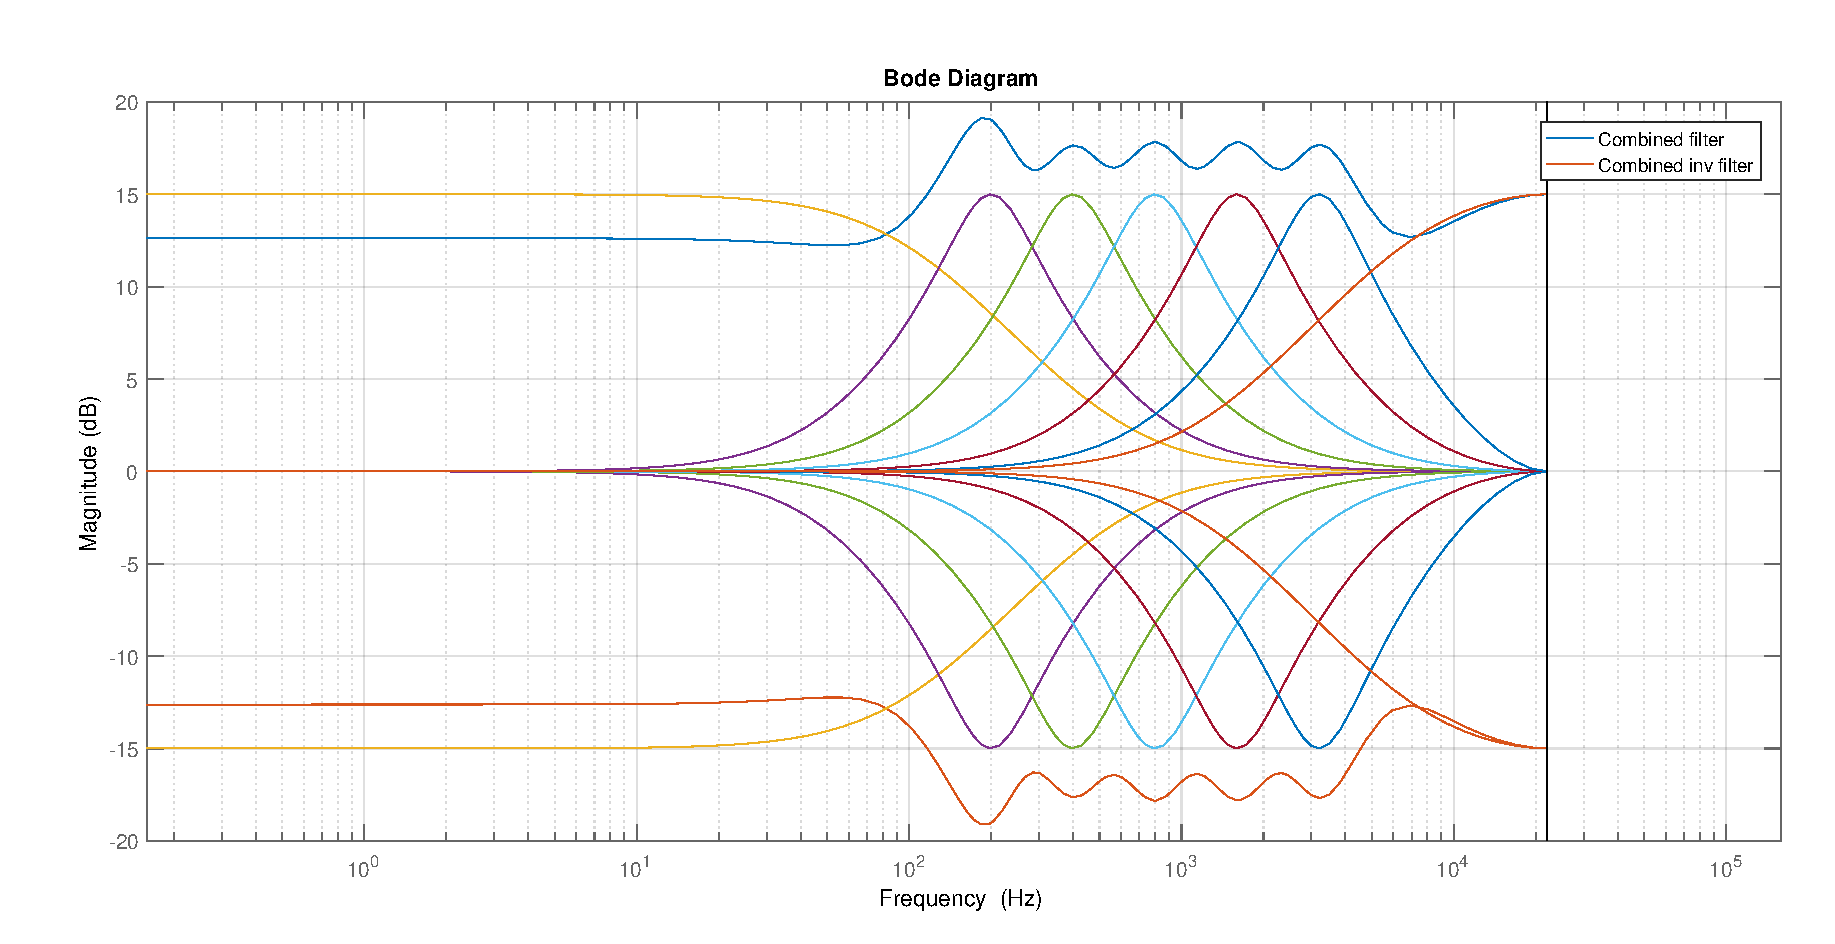
\includegraphics[width=\textwidth]{eq_z_domain_final.pdf}
        \caption{Bodeplot of the final equalizer's dynamic range in z-domain, with all bands fully amplified and fully attenuated.}
        \label{fig:eq_z_domain_final}
  \end{figure}
  
\subsection{Implementation of the equalizer}
When implementing the equalizer on the\gls{dsp} the amplifying part of the equalizer will be implemented first. This is because the amplifying part is the simplest one, since fewer coefficients have to be allocated in the \gls{dsp} memory. As seen in \autoref{eq:z_to_n7} the gain value, $G$, can be seen as an isolated scalar, which is multiplied on the coefficient fraction and a data value. Therefore e.g. $\frac{a_{peak1}}{b_{peak1}}$ can be written as a constant in the \gls{dsp}, no matter how much the specific band should amplify. This is not the case for the attenuating part of the equalizer, since the gain,$G$, is changing e.g. the coefficient $b_{peak1-cut}$, which is a denominator in \autoref{eq:z_to_n_peak_att}. 
The equalizer is implemented using 16-bits precision and the main algorithm of the amplifying part of the equalizer is shown in \autoref{code:eq_code}. 

\includeCode{equalizer.asm}{assembly}{61}{82}{The filter algorithm in the equalizer}{code:eq_code}{code/design/}

The code shows the implementation of one filter as for example the filter represented in \autoref{eq:z_to_n7}. Line 68 does the calculation $- \frac{b_{peak3}}{b_{peak1}} \cdot y_{peak}[n-2]$ and stores it in AC0. Line 69 does the calculation $-  \frac{b_{peak2}}{b_{peak1}} \cdot y_{peak}[n-1]$, adds it to what is already in AC0, and moves $y_{peak}[n-1]$ to $y_{peak}[n-2]$. This way the algorithm does the calculation of $y_{peak}[n]$. In line 74 $y_{peak}[n]$ is stored in $y_{peak}[n-1]$ to be ready to the next sample.  
Line 71 is special for the amplifying filters, because the coefficient in this line is zero, because \autoref{eq:z_to_n7} does not use $x[n-1]$ in its calculations. 
In \autoref{code:eq_code_parallel} the implementation of the block diagram in \autoref{fig:eq_parallel} is seen.

\includeCode{equalizer.asm}{assembly}{84}{118}{The implementation of \autoref{fig:eq_parallel}}{code:eq_code_parallel}{code/design/}

Line 117 is where all the outputs of the seven filters are added to the direct input.

In \autoref{fig:memory_map_eq} a memory map for the equalizer is shown. It consists of three coefficient buffers and three data buffers. 

\begin{figure}[htbp!]
\centering
\begin{picture}(0,0)%
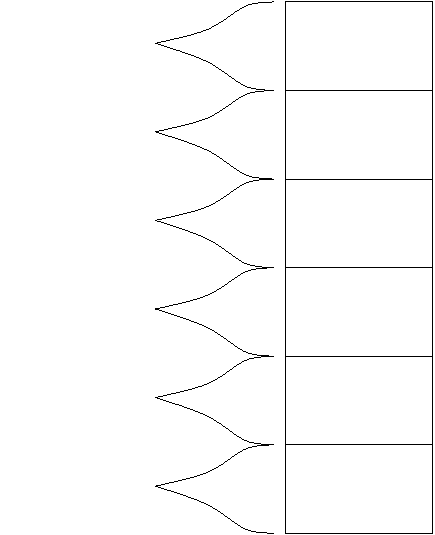
\includegraphics{equalizer_mem_map.pdf}%
\end{picture}%
\setlength{\unitlength}{4144sp}%
%
\begingroup\makeatletter\ifx\SetFigFont\undefined%
\gdef\SetFigFont#1#2#3#4#5{%
  \reset@font\fontsize{#1}{#2pt}%
  \fontfamily{#3}\fontseries{#4}\fontshape{#5}%
  \selectfont}%
\fi\endgroup%
\begin{picture}(3312,4074)(9076,-4798)
\put(11476,-1996){\makebox(0,0)[lb]{\smash{{\SetFigFont{12}{14.4}{\rmdefault}{\mddefault}{\updefault}{\color[rgb]{0,0,0}0x471E}%
}}}}
\put(11476,-3661){\makebox(0,0)[lb]{\smash{{\SetFigFont{12}{14.4}{\rmdefault}{\mddefault}{\updefault}{\color[rgb]{0,0,0}0x474D}%
}}}}
\put(11476,-4336){\makebox(0,0)[lb]{\smash{{\SetFigFont{12}{14.4}{\rmdefault}{\mddefault}{\updefault}{\color[rgb]{0,0,0}0x4764}%
}}}}
\put(11476,-4696){\makebox(0,0)[lb]{\smash{{\SetFigFont{12}{14.4}{\rmdefault}{\mddefault}{\updefault}{\color[rgb]{0,0,0}0x477B}%
}}}}
\put(11476,-4021){\makebox(0,0)[lb]{\smash{{\SetFigFont{12}{14.4}{\rmdefault}{\mddefault}{\updefault}{\color[rgb]{0,0,0}0x4763}%
}}}}
\put(9091,-1096){\makebox(0,0)[lb]{\smash{{\SetFigFont{12}{14.4}{\rmdefault}{\mddefault}{\updefault}{\color[rgb]{0,0,0}Coeff EQ 1,2,3}%
}}}}
\put(9181,-4471){\makebox(0,0)[lb]{\smash{{\SetFigFont{12}{14.4}{\rmdefault}{\mddefault}{\updefault}{\color[rgb]{0,0,0}Data shelving}%
}}}}
\put(9271,-3796){\makebox(0,0)[lb]{\smash{{\SetFigFont{12}{14.4}{\rmdefault}{\mddefault}{\updefault}{\color[rgb]{0,0,0}Data EQ 4,5}%
}}}}
\put(9136,-3121){\makebox(0,0)[lb]{\smash{{\SetFigFont{12}{14.4}{\rmdefault}{\mddefault}{\updefault}{\color[rgb]{0,0,0}Data EQ 1,2,3}%
}}}}
\put(9136,-2446){\makebox(0,0)[lb]{\smash{{\SetFigFont{12}{14.4}{\rmdefault}{\mddefault}{\updefault}{\color[rgb]{0,0,0}Coeff shelving}%
}}}}
\put(9226,-1771){\makebox(0,0)[lb]{\smash{{\SetFigFont{12}{14.4}{\rmdefault}{\mddefault}{\updefault}{\color[rgb]{0,0,0}Coeff EQ 4,5}%
}}}}
\put(11476,-1321){\makebox(0,0)[lb]{\smash{{\SetFigFont{12}{14.4}{\rmdefault}{\mddefault}{\updefault}{\color[rgb]{0,0,0}0x4707}%
}}}}
\put(11476,-1636){\makebox(0,0)[lb]{\smash{{\SetFigFont{12}{14.4}{\rmdefault}{\mddefault}{\updefault}{\color[rgb]{0,0,0}0x4708}%
}}}}
\put(11476,-2311){\makebox(0,0)[lb]{\smash{{\SetFigFont{12}{14.4}{\rmdefault}{\mddefault}{\updefault}{\color[rgb]{0,0,0}0x471F}%
}}}}
\put(11476,-2671){\makebox(0,0)[lb]{\smash{{\SetFigFont{12}{14.4}{\rmdefault}{\mddefault}{\updefault}{\color[rgb]{0,0,0}0x4735}%
}}}}
\put(11476,-2986){\makebox(0,0)[lb]{\smash{{\SetFigFont{12}{14.4}{\rmdefault}{\mddefault}{\updefault}{\color[rgb]{0,0,0}0x4736}%
}}}}
\put(11476,-3346){\makebox(0,0)[lb]{\smash{{\SetFigFont{12}{14.4}{\rmdefault}{\mddefault}{\updefault}{\color[rgb]{0,0,0}0x474C}%
}}}}
\put(11476,-961){\makebox(0,0)[lb]{\smash{{\SetFigFont{12}{14.4}{\rmdefault}{\mddefault}{\updefault}{\color[rgb]{0,0,0}0x46F1}%
}}}}
\end{picture}%

\caption{Memory map for the equalizer.}
		\label{fig:memory_map_eq}
\end{figure}

%Raised Cosine

%The interference effects on the side lying bandpass filter can easily be avoided by using an digital equalizer with third-octave raised cosine characteristics. The difference between the  bandpass filter characteristics and the one with a raised-cosine are shown in \autoref{fig:raised_cosine_vs_traditional}
%
%\begin{figure} [htbp]
% \centering
%  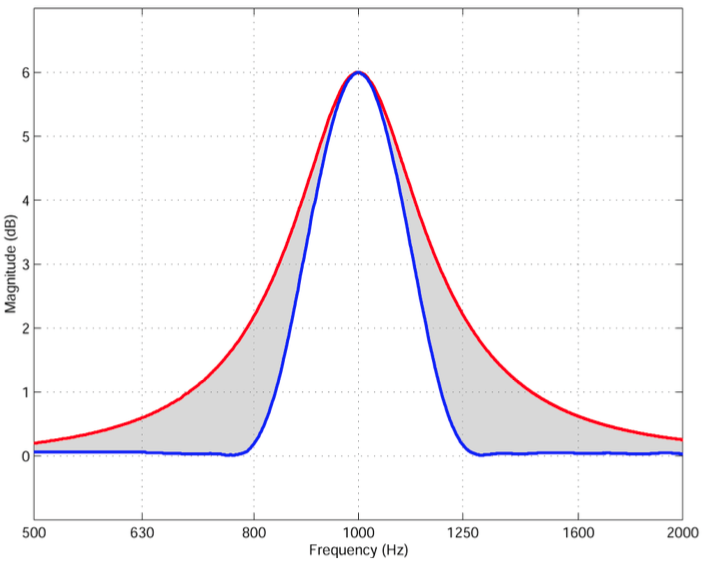
\includegraphics[width=0.7\textwidth]{raised_cosine_vs_traditional}
%  \caption{The photo shows the raised cosine bandpass filter characteristics versus traditional characteristics of third-octave bandpass filter \citep{nordic}
%  }
%  \label{fig:raised_cosine_vs_traditional}
%\end{figure}
%
%
%
%When using third-octave raised cosine bandpass filter, it is possible to make an equalizer where neighboring filters do not interfere with each other, or explained i another way, they interfere the right way, because a raised cosine filter does not leak into other third-octave bands like the traditional filter does. With this kind of filter it is possible to make a perfectly flat frequency response, and it is very close to an ideal equalizer. The \autoref{fig:raised_cosine_respond} shows the frequency response of a third-octave raised cosine equalizer designed by Dolby lake with the same gain and frequency settings as the analog equalizer at \autoref{fig:analog_equalizer}.
%
%\begin{figure} [htbp]
% \centering
%  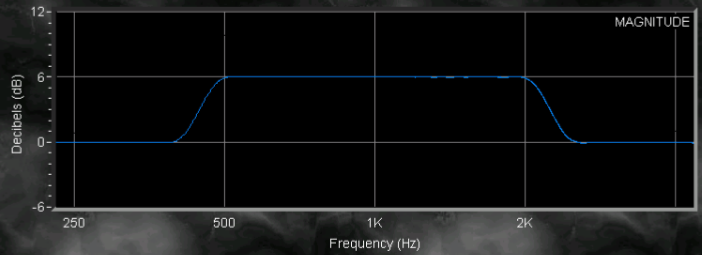
\includegraphics[width=0.8\textwidth]{raised_cosine_respond}
%  \caption{The photo shows an third-octave raised cosine equalizer frequency response  \citep{nordic}
%  }
%  \label{fig:raised_cosine_respond}
%\end{figure}
%
%
%The equalizer is used to compensate for the changes in sound due to different room characteristics, because the sound can be completely different in different rooms. The room characteristics will or can amplify or attenuate some frequency, and therefore the equalizer is very important to adjust the frequency in every new room.\citep{howtogeek} 

%\section{Design of the Wah-Wah Effect}

\subsection{Choice of the Bandpass Filter}

The block diagram of the wah-wah effect has been presented in the analysis and is shown again below in  \autoref{fig:wah_diag_2}:

\begin{figure} [htbp]
	\centering
	\begin{picture}(0,0)%
	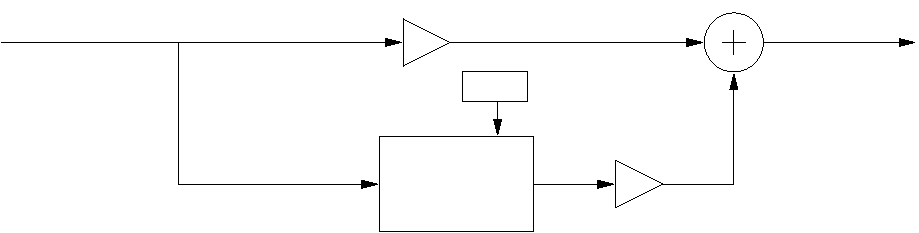
\includegraphics{wah_diag.pdf}%
	\end{picture}%
	\setlength{\unitlength}{4144sp}%
	%
	\begingroup\makeatletter\ifx\SetFigFont\undefined%
	\gdef\SetFigFont#1#2#3#4#5{%
		\reset@font\fontsize{#1}{#2pt}%
		\fontfamily{#3}\fontseries{#4}\fontshape{#5}%
		\selectfont}%
	\fi\endgroup%
	\begin{picture}(6999,1770)(2689,-2233)
	\put(6841,-1591){\textit{Wah-Wah Gain}}%
	\put(5626,-2041){$Filter$}%
	\put(6136,-1186){\textit{LFO or Pedal}}%
	\put(2746,-646){$Input$}%
	\put(8686,-646){$Output$}%
	\put(5626,-1816){$Bandpass-$}%
	\put(5986,-646){$Gain$}%
	\end{picture}%
	\caption{Block diagram of the wah-wah effect}
	\label{fig:wah_diag_2}
\end{figure}

Different types of filters can be implemented using the first and second order allpass filters. In the case of the wah-wah, it can be inferred from \autoref{fig:wah_diag_2} that a bandpass filter is needed as a part of the feedforward loop. 

With a first order allpass filter, it is possible to design a circuit to make lowpass- and highpass- filters, but not bandpass- or bandreject- filters. Thus, the focus will be on the second order allpass filter, since a second order allpass filter can be used to obtain the bandpass filter, which is needed. \autoref{fig:wah_allpass} shows the block diagram of the second order allpass filter.

\begin{figure} [htbp]
	\centering
	\begin{picture}(0,0)%
	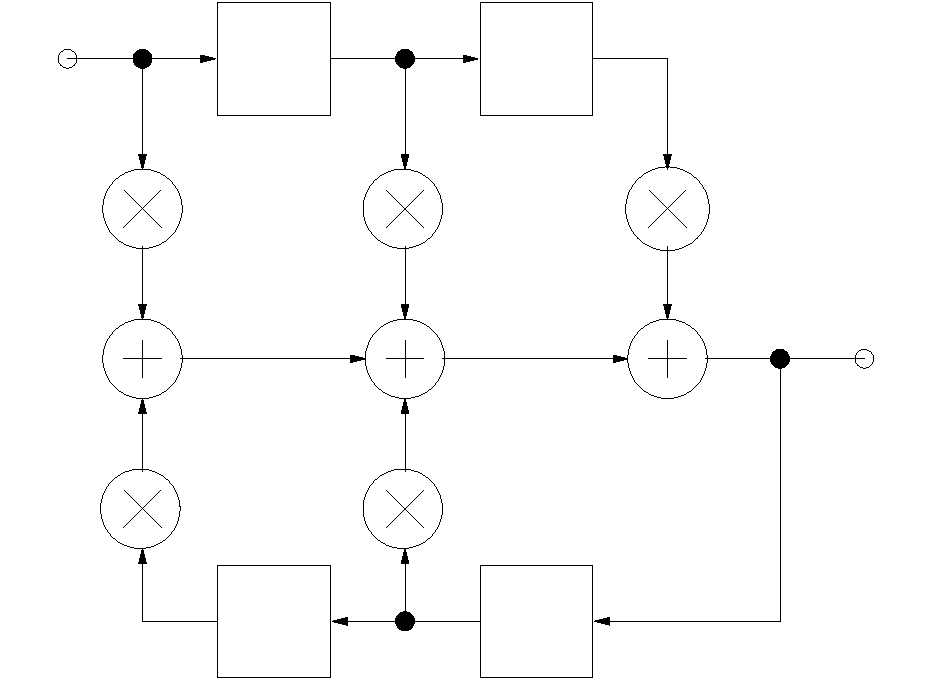
\includegraphics{wah_allpass.pdf}%
	\end{picture}%
	\setlength{\unitlength}{3947sp}%
	%
	\begingroup\makeatletter\ifx\SetFigFont\undefined%
	\gdef\SetFigFont#1#2#3#4#5{%
		\reset@font\fontsize{#1}{#2pt}%
		\fontfamily{#3}\fontseries{#4}\fontshape{#5}%
		\selectfont}%
	\fi\endgroup%
	\begin{picture}(7524,5424)(1411,-5923)
	\put(3001,-2236){-c}%

	\put(3526,-1036){T}%

	\put(5626,-1036){T}%

	\put(5626,-5536){T}%
	
	\put(3526,-5536){T}%
	
	\put(8551,-3436){y(n)}%
	
	\put(1426,-1036){x(n)}%
	
	\put(4426,-811){x(n-1)}%
	
	\put(6451,-811){x(n-2)}%
	
	\put(2251,-5686){y(n-2)}%
	
	\put(4426,-5761){y(n-1)}%
	
	\put(7201,-2236){1}%
	
	\put(3001,-4636){c}%
	
	\put(5101,-4636){-d(1-c)}%
	
	\put(5101,-2236){d(1-c)}%
	
	\end{picture}%
	\caption{Block diagram for a second-order allpass filter \citep{DAFX}}
	\label{fig:wah_allpass}
\end{figure}

The transfer function in Z-domain can be inferred from \autoref{fig:wah_allpass} :

\begin{equation} \label{wah_z_equation}
		A(z) = \frac{-c+d(1-c)z^{-1}+z^{-2}}{1+d(1-c)z^{-1}-cz^{-2}}
		\end{equation}
		
where:

\begin{equation}
	c = \frac{tan(\pi f_{b}/f_{s})-1}{tan(\pi f_{b}/f_{s})+1}
	\end{equation}

and

\begin{equation}
	d = -cos(2\pi f_{c}/f_{s})
	\end{equation}

$f_{s}$ represents the sampling frequency, $f_{c}$ the cutoff frequency and $f_{b}$ the ??. The factor $d$ grants control over the cutoff frequency while the factor $c$ permits the change in bandwidth. \\

From the \autoref{wah_z_equation}, it is possible to obtain the equation in the discrete time-domain that can then be used for digital implementation which includes Matlab simulations and so on. 
\begin{equation}\label{wah_eq_1}
	y(n) = -cx(n) + d(1-c)x(n-1) + x(n-2) - d(1-c)y(n-1) + cy(n-2)  
\end{equation}


Using the allpass filter presented above, it is possible to create a bandpass filter by simply summing the input signal with the one coming from the allpass filter, a block diagram that illustrates the design for a better understanding is in \autoref{fig:wah_bandpass}:

\begin{figure} [htbp]
	\centering
	\begin{picture}(0,0)%
	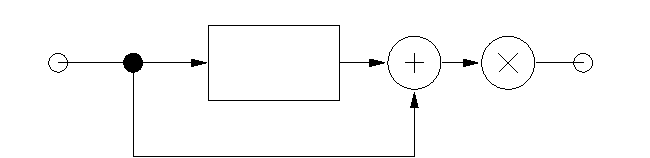
\includegraphics{wah_bandpass.pdf}%
	\end{picture}%
	\setlength{\unitlength}{3947sp}%
	%
	\begingroup\makeatletter\ifx\SetFigFont\undefined%
	\gdef\SetFigFont#1#2#3#4#5{%
		\reset@font\fontsize{#1}{#2pt}%
		\fontfamily{#3}\fontseries{#4}\fontshape{#5}%
		\selectfont}%
	\fi\endgroup%
	\begin{picture}(5199,1257)(3136,-2923)
	\put(5926,-2011){\textit{y(n)}}%
	
	\put(5176,-2236){\textit{A(z)}}%
	
	\put(7051,-1861){\textit{1/2}}%
	
	\put(3050,-2236){$x_{b}(n)$}%
	
	\put(7951,-2236){$y_{b}(n)$}%
	
	\put(4276,-2011){\textit{x(n)}}%
	
	
	\end{picture}%
	
	\caption{Block diagram for a second-order bandpass filter \citep{DAFX}}
	\label{fig:wah_bandpass}
\end{figure}

From \autoref{fig:wah_bandpass}, the transfer function of the bandpass filter is then:

\begin{equation}
 	H(z) = 1/2 (1 + A(z))
\end{equation}

The discrete time equation can also be inferred:

\begin{equation}\label{wah_eq_2}
		y_{b} = \frac{1}{2} (x(n) + y(n))
\end{equation}

since $y(n)$ is known from \autoref{wah_eq_1}, \autoref{wah_eq_2} can be re-written as :

\begin{equation}
			y_{b}(n) = \frac{1}{2} ((1-c)x(n) + d(1-c)x(n-1) + x(n-2) - d(1-c)y(n-1) + cy(n-2) )
\end{equation}
%%\setlength{\unitlength}{1973sp}% un scaled 3947sp
%%	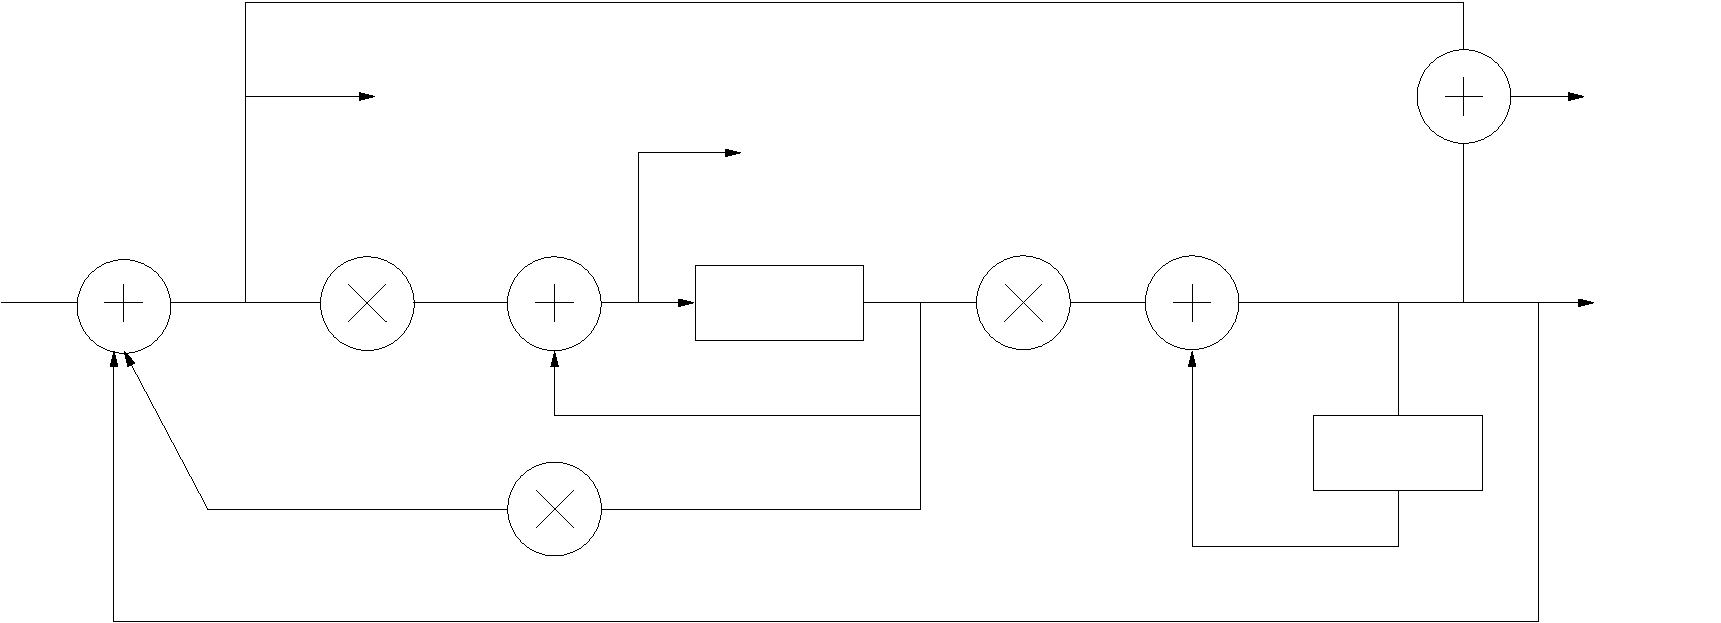
\includegraphics[width=1\textwidth]{wah_bandpass_second.pdf}%
\subsection{Bandpass filter using Chamberlin}

\autoref{fig:wah_bandpass_second} shows the general topology of the Chamberlin state variable filter.

\begin{figure} [htbp]
	\centering
		\begin{picture}(0,0)%
		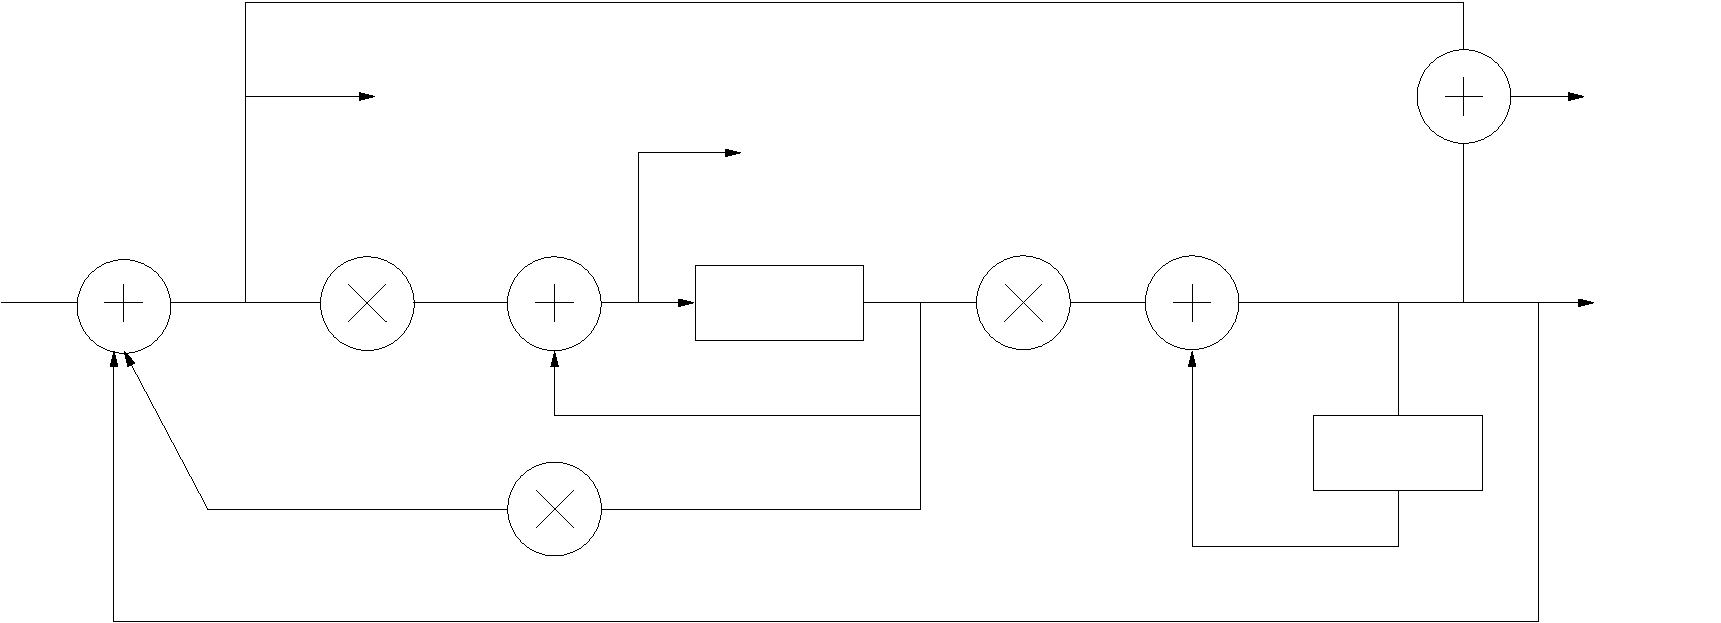
\includegraphics[width=1\textwidth]{wah_bandpass_second.pdf}%
		\end{picture}%
		\setlength{\unitlength}{1973sp}% un scaled 3947sp
		%
		\begingroup\makeatletter\ifx\SetFigFont\undefined%
		\gdef\SetFigFont#1#2#3#4#5{%
			\reset@font\fontsize{#1}{#2pt}%
			\fontfamily{#3}\fontseries{#4}\fontshape{#5}%
			\selectfont}%
		\fi\endgroup%
		\begin{picture}(13761,4974)(139,-5173)
		\put(4551,-4361){q}%
		
		\put(6001,-2786){$z^{-1}$}%
		
		\put(10951,-3986){$z^{-1}$}%
		
		\put(3226,-1036){Highpass}%
		
		\put(6076,-1486){Bandpass}%
		
		\put(12976,-2686){Lowpass}%
		
		\put(12901,-1036){Bandreject}%
		
		\put(1426,-3136){-}%
		
		\put(826,-3136){-}%
		
		\put(2751,-2786){f}%
		
		\put(7876,-2786){f}%
		
		\end{picture}%
	
	\caption{Block diagram the Chamberlin state variable filter topology \citep{}}
	\label{fig:wah_bandpass_second}
\end{figure}

This topology can be used to obtain a bandpass filter with a variable center frequency. 

The factor $f$ that is shown on \autoref{fig:wah_bandpass_second} is the frequency control coefficient defined as in the following equation:

\begin{equation}
      f = 2 \cdot sin(\frac{\pi \cdot f_{c}}{f_{s}})
\end{equation}

The factor $q$ is defined as the inverse of the Q-factor.

\begin{equation}
			q = \frac{1}{Q}
\end{equation}

The minimum value for the Q-factor is normally 0.5 while the maximum value of the frequency control coefficient $f$ is 1. 

The Chamberlin topology has different advantages; it lets the user control the center frequency and the Q-factor by controlling the previously stated characteristic coefficients. The range of the working frequencies can be changed easily by changing the gain values. Thus it is this topology that is going to be used due to its easy application. \\

The complexity of one sample calculation using this filter is five additions and three multiplications according to the book \textit{Musical Applications of Microprocessors}. 

The equations that give the output values of the filters are the following:

\begin{equation}
   			y_{1}[n] = y_{1}[n-1] + f \cdot y_{2}[n-1]
\end{equation}

\begin{equation}
            y_{3}[n] = x[n]  - y_{1}[n]   - q \cdot y_{2}[n-1]
\end{equation}

\begin{equation}
           y_{2}[n] = f \cdot y_{3}[n] + y_{2}[n-1]
\end{equation}

Where $y_{1}$ is the lowpass output, $y_{2}$ the bandpass output and $y_{3}$ the highpass output. \\
the Q-factor $q$ can also be defined as the double of the damping ratio. \\

The Wah-Wah effect output is then the sum of the bandpass filter and the direct input. Those two values can be multiplied by a certain gain. \\

\subsection{Matlab Simulation}

Using the equations found in the previous subsection, it is possible to implement the effect digitally. 

\begin{lstlisting}[language=Matlab, caption= Matlab code for wah-wah effect]

%% Wah-Wah Effect 

clear all;
filename = 'guitartune.wav'; 
%The filename is inserted here, should be in the same directory as the
%codefile.
[input, fs] = audioread(filename);
%input samples and sample rate are extracted from the file.
input = input / (max(abs(input)));
%the input is rescaled in order to have values between -1 and 1.


%Varitations of the center frequency of the bandpass filter:

minomega0 = 500;
maxomega0 = 3000;
yb = (1:1:length(input));
yl = (1:1:length(input));
yh = (1:1:length(input));
output = (1:1:length(input));
%Auto-Wah Frequency, how fast does the bandpass filter travels through the
%spectrum

autofreq = 150;

fb = 200 * 2 * pi / fs;

if fb > length(input)
error('Chosen bandwidth very big')
end

%Divide by the sampling frequency to pass from changes per second to
%changes per sample

change = autofreq / fs;

%Create a table that contains all the values of the center frequency

Fc = minomega0:change:maxomega0;


%Q = Fc/fb %the Qfactor

q = 2*0.05;

if length(Fc) < length(input)
 error('High Auto-Wah Frequency, please decrease the value')
else 
 if length (Fc) > length(input)
  Fc = Fc(1:length(input));
 end
end

f = 2 * sin((pi * Fc)/fs);

g1 = 0.7;
g2 = 2;

yl(1) = 0;
yh(1) = input(1);
yb(1) = f(1) * yh(1);

for i=2:1:length(input)
 yl(i) = yl(i-1) + f(i) * yb(i-1);
 yh(i) = input(i) - yl(i) - q * yb(i-1);
 yb(i) = f(i) * yh(i) + yb(i-1);
 output(i) = g1*input(i) + g2*yb(i);
end

output = output / (max(abs(output)));

audiowrite('wahwah_out.wav',output,fs);


plot(input,'r') %plotting the input samples in blue on the same fig.


hold on
grid
plot(output,'b') %plotting the output samples in red.

\end{lstlisting}

sources:
http://www.earlevel.com/main/2003/03/02/the-digital-state-variable-filter/ and the slides (to be added after)


%%
 \graphicspath{{figures/tests/}}
\part{Tests}\label{pt:tests}
\section{Test of the converters}
In this part, all the requirements related to the converters will be tested if they are fulfilled. 


\subsection{Test of \autoref{req:ADC_resolution}}
According to \autoref{req:ADC_resolution}, the \gls{adc} must have a resolution of at least 10 bits. In \autoref{sec:dsp_description} it is seen that the TMS320C5515 eZdsp development board has an \gls{adc} with a resolution of \SI{92}{\decibel} (16-bits). Thus the requirement is fulfilled.  

\subsection{Test of \autoref{req:ADC_Fs}}
According to \autoref{req:ADC_Fs}, the \gls{adc} must have a sampling frequency of at least \SI{8.8}{\kilo\hertz}. In \autoref{sec:dsp_description} it is seen that the TMS320C5515 eZdsp development board has an \gls{adc} with a sampling frequency, which can be set from \SI{8}{\kilo\hertz} to \SI{192}{\kilo\hertz}. Thus the requirement is fulfilled.

\subsection{Test of \autoref{req:DAC_resolution}}
According to \autoref{req:ADC_resolution}, the \gls{dac} must have a resolution of at least 10 bits. In \autoref{sec:dsp_description} it is seen that the TMS320C5515 eZdsp development board has a \gls{dac} with a resolution of \SI{100}{\decibel} (17-bits). Thus the requirement is fulfilled.  

\subsection{Test of \autoref{req:DAC_Fs}}
According to \autoref{req:ADC_Fs}, the \gls{adc} must have a sampling frequency of at least \SI{8.8}{\kilo\hertz}. In \autoref{sec:dsp_description} it is seen that the TMS320C5515 eZdsp development board has a \gls{dac} with a sampling frequency, which can be set from \SI{8}{\kilo\hertz} to \SI{192}{\kilo\hertz}. Thus the requirement is fulfilled.
 
\subsection{Test review of the converter}
In this subsection, a short review will be shown of the converter test.

\begin{table}[H]
\centering
\caption{Recap of the requirements fulfillments for the converter test}
\label{test_of_converter_table}
\begin{tabular}{|l|l|}
\hline
\rowcolor[HTML]{9B9B9B} 
\textbf{Requirement} & \textbf{Fulfillment State} \\ \hline
\textbf{\ref{req:ADC_resolution}}    & \cmark                     \\ \hline
\textbf{\ref{req:ADC_Fs}}    & \cmark                     \\ \hline
\textbf{\ref{req:DAC_resolution}}    & \cmark                      \\ \hline
\textbf{\ref{req:DAC_Fs}}    & \cmark                      \\ \hline
\end{tabular}
\end{table}

\newpage
\section{Pre-amplifier test}
This section will present the tests of all requirements related to the \gls{preamp}. 


\subsection{\autoref{req:preamp1}}
For \autoref{req:preamp1}, a test was made to ensure that the \gls{preamp} does not change the signal amplitude more than $\pm$\SI{1}{\decibel} between 20 Hz and 20 kHz. A test was made and is described in \autoref{app:preamp_frequency_response} and the result is seen in \autoref{fig:tests:appendix:amplitude}.

\begin{figure}[htbp!]
	\centering
		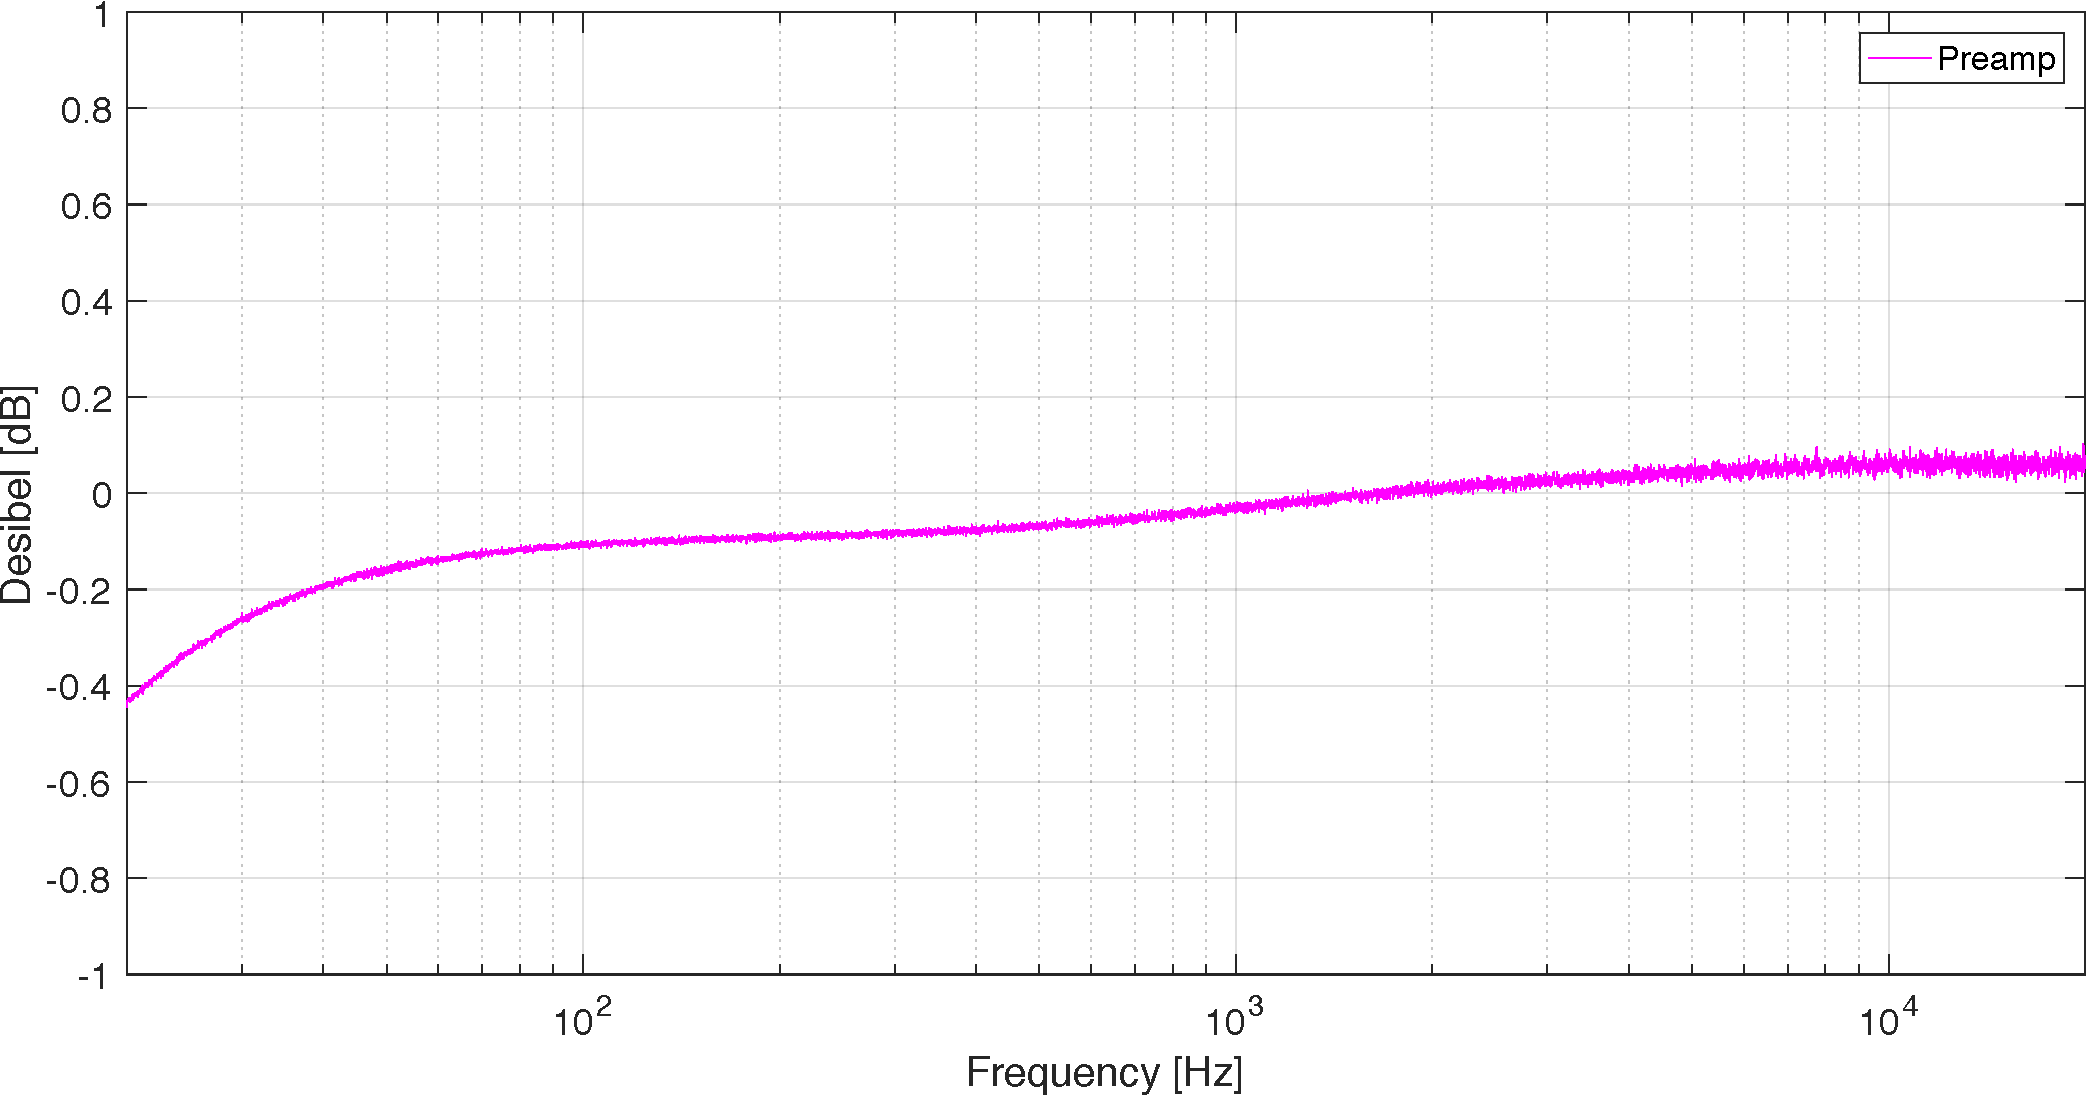
\includegraphics[width=1\textwidth]{preamp_frequency_responce.pdf}
		\caption{Measurement of the frequency response of the \gls{preamp}.}
		\label{fig:tests:appendix:amplitude}
\end{figure}

The amplitude is within $\pm$\SI{1}{\decibel} so \autoref{req:preamp1} is approved.


\subsection{\autoref{req:preamp2}}
According to \autoref{req:preamp2} the input impedance of  the \gls{preamp} must be at least 10 times the output impedance of the guitar. The requirement is assumed approved since the input impedance of an \gls{opamp} is normally between $10^5$ to $10^{12}$ $\Omega$, without a feedback loop. \autoref{eq:preamp_result} is therefore assumed correct and therefore the input impedance of the \gls{preamp} is \SI{1}{\mega\ohm}.
%According to \autoref{req:preamp2}, a test was made to ensure that the \gls{preamp} have an input impedance 10 times higher than the highest output impedance of the guitar. According to \autoref{app:output_impedance} and the requirements the \gls{preamp} shall have an input impedance of at least \SI{730.8}{\kilo\ohm}. To ensure that the input impedance is more than \SI{730.8}{\mega\ohm}. The input impedance of the \gls{opamp} was measured, and the result is to \SI{9.18}{\mega\ohm} according to \autoref{app:opamp_impedance}. Applying the input impedance to the following \autoref{eq:tests:preamp_result}, where $A$ is at least \SI{70}{\decibel}, according to \citep{TS464}.  
%
%\begin{equation}\label{eq:tests:preamp_result}
%        Z_{In_{G1}} = R_{Bias} \parallel ((Z_i + Z_{i \beta}) \cdot (1+\beta \cdot A)) \simeq R_{Bias}
%        \addunit{\si{\ohm}}
%    \end{equation}
%
%where the value from \autoref{label_Pre-amplifier} is applied as following \autoref{eq:tests:preamp_result_value}.



%
%\begin{subequations}\label{eq:tests:preamp_result_value}
%\begin{equation}
%        Z_{In_{G1}} = \SI{1}{\mega\ohm} \parallel ((\SI{9.18}{\mega\ohm} + 2550 \ohm) \cdot (1+ 0.5 \cdot 3162)) \simeq R_{Bias}
%        \addunit{\si{\ohm}}
%    \end{equation}
%\centering
%$\Updownarrow$
%\begin{equation}
%        Z_{In_{G1}} = \SI{1}{\mega\ohm} \parallel \SI{14.53}{\giga\ohm}  \simeq R_{Bias}
%        \addunit{\si{\ohm}}
%    \end{equation}
%    $\Updownarrow$
%\begin{equation}
%        \SI{999.9}{\kilo\ohm} = \SI{1}{\mega\ohm} \parallel \SI{14.53}{\giga\ohm} 
%        \addunit{\si{\ohm}}
%    \end{equation}
% \end{subequations}
%
%The calculated input impedance is higher than the required input impedance, so \autoref{req:preamp2} is approved.

\subsection{\autoref{req:preamp3}}
According to \autoref{req:preamp3} the output impedance of the preamp must be one tenth of the input impedance of the \gls{dsp}. The requirement is approved since the output impedance of an \gls{opamp} is normally between \SI{50}{\ohm} to \SI{200}{\ohm}, without a feedback loop. The input impedance of the \gls{dsp} is \SI{20}{\kilo\ohm} and \autoref{eq:preamp_zout_out} is therefore assumed correct and thus the requirement is fulfilled \citep{TLV320AIC3204}.  

\subsection{\autoref{req:preamp4}}
The \gls{preamp} is designed to be supplied by a 5 to 9 voltage supply, and the \gls{preamp} will be supplied from a \SI{9}{\volt} battery. The \autoref{req:preamp4} is therefore approved.

\subsection{\autoref{req:preamp5} and \autoref{req:preamp6}}
According to \autoref{req:preamp6}, a test was made to ensure that the \gls{preamp} \gls{pcb} including cable mount fits into the jack connector house. \autoref{fig:tests:preamp_pcb} shows the \gls{pcb} mounted on the jack connector and the cable is mounted on the \gls{preamp}. 

 

\autoref{fig:tests:preamp_jack} shows the \gls{preamp} \gls{pcb} mounted inside the jack connector house.

\begin{figure}[htbp]
\centering
\begin{subfigure}[htbp]{0.35\textwidth}
		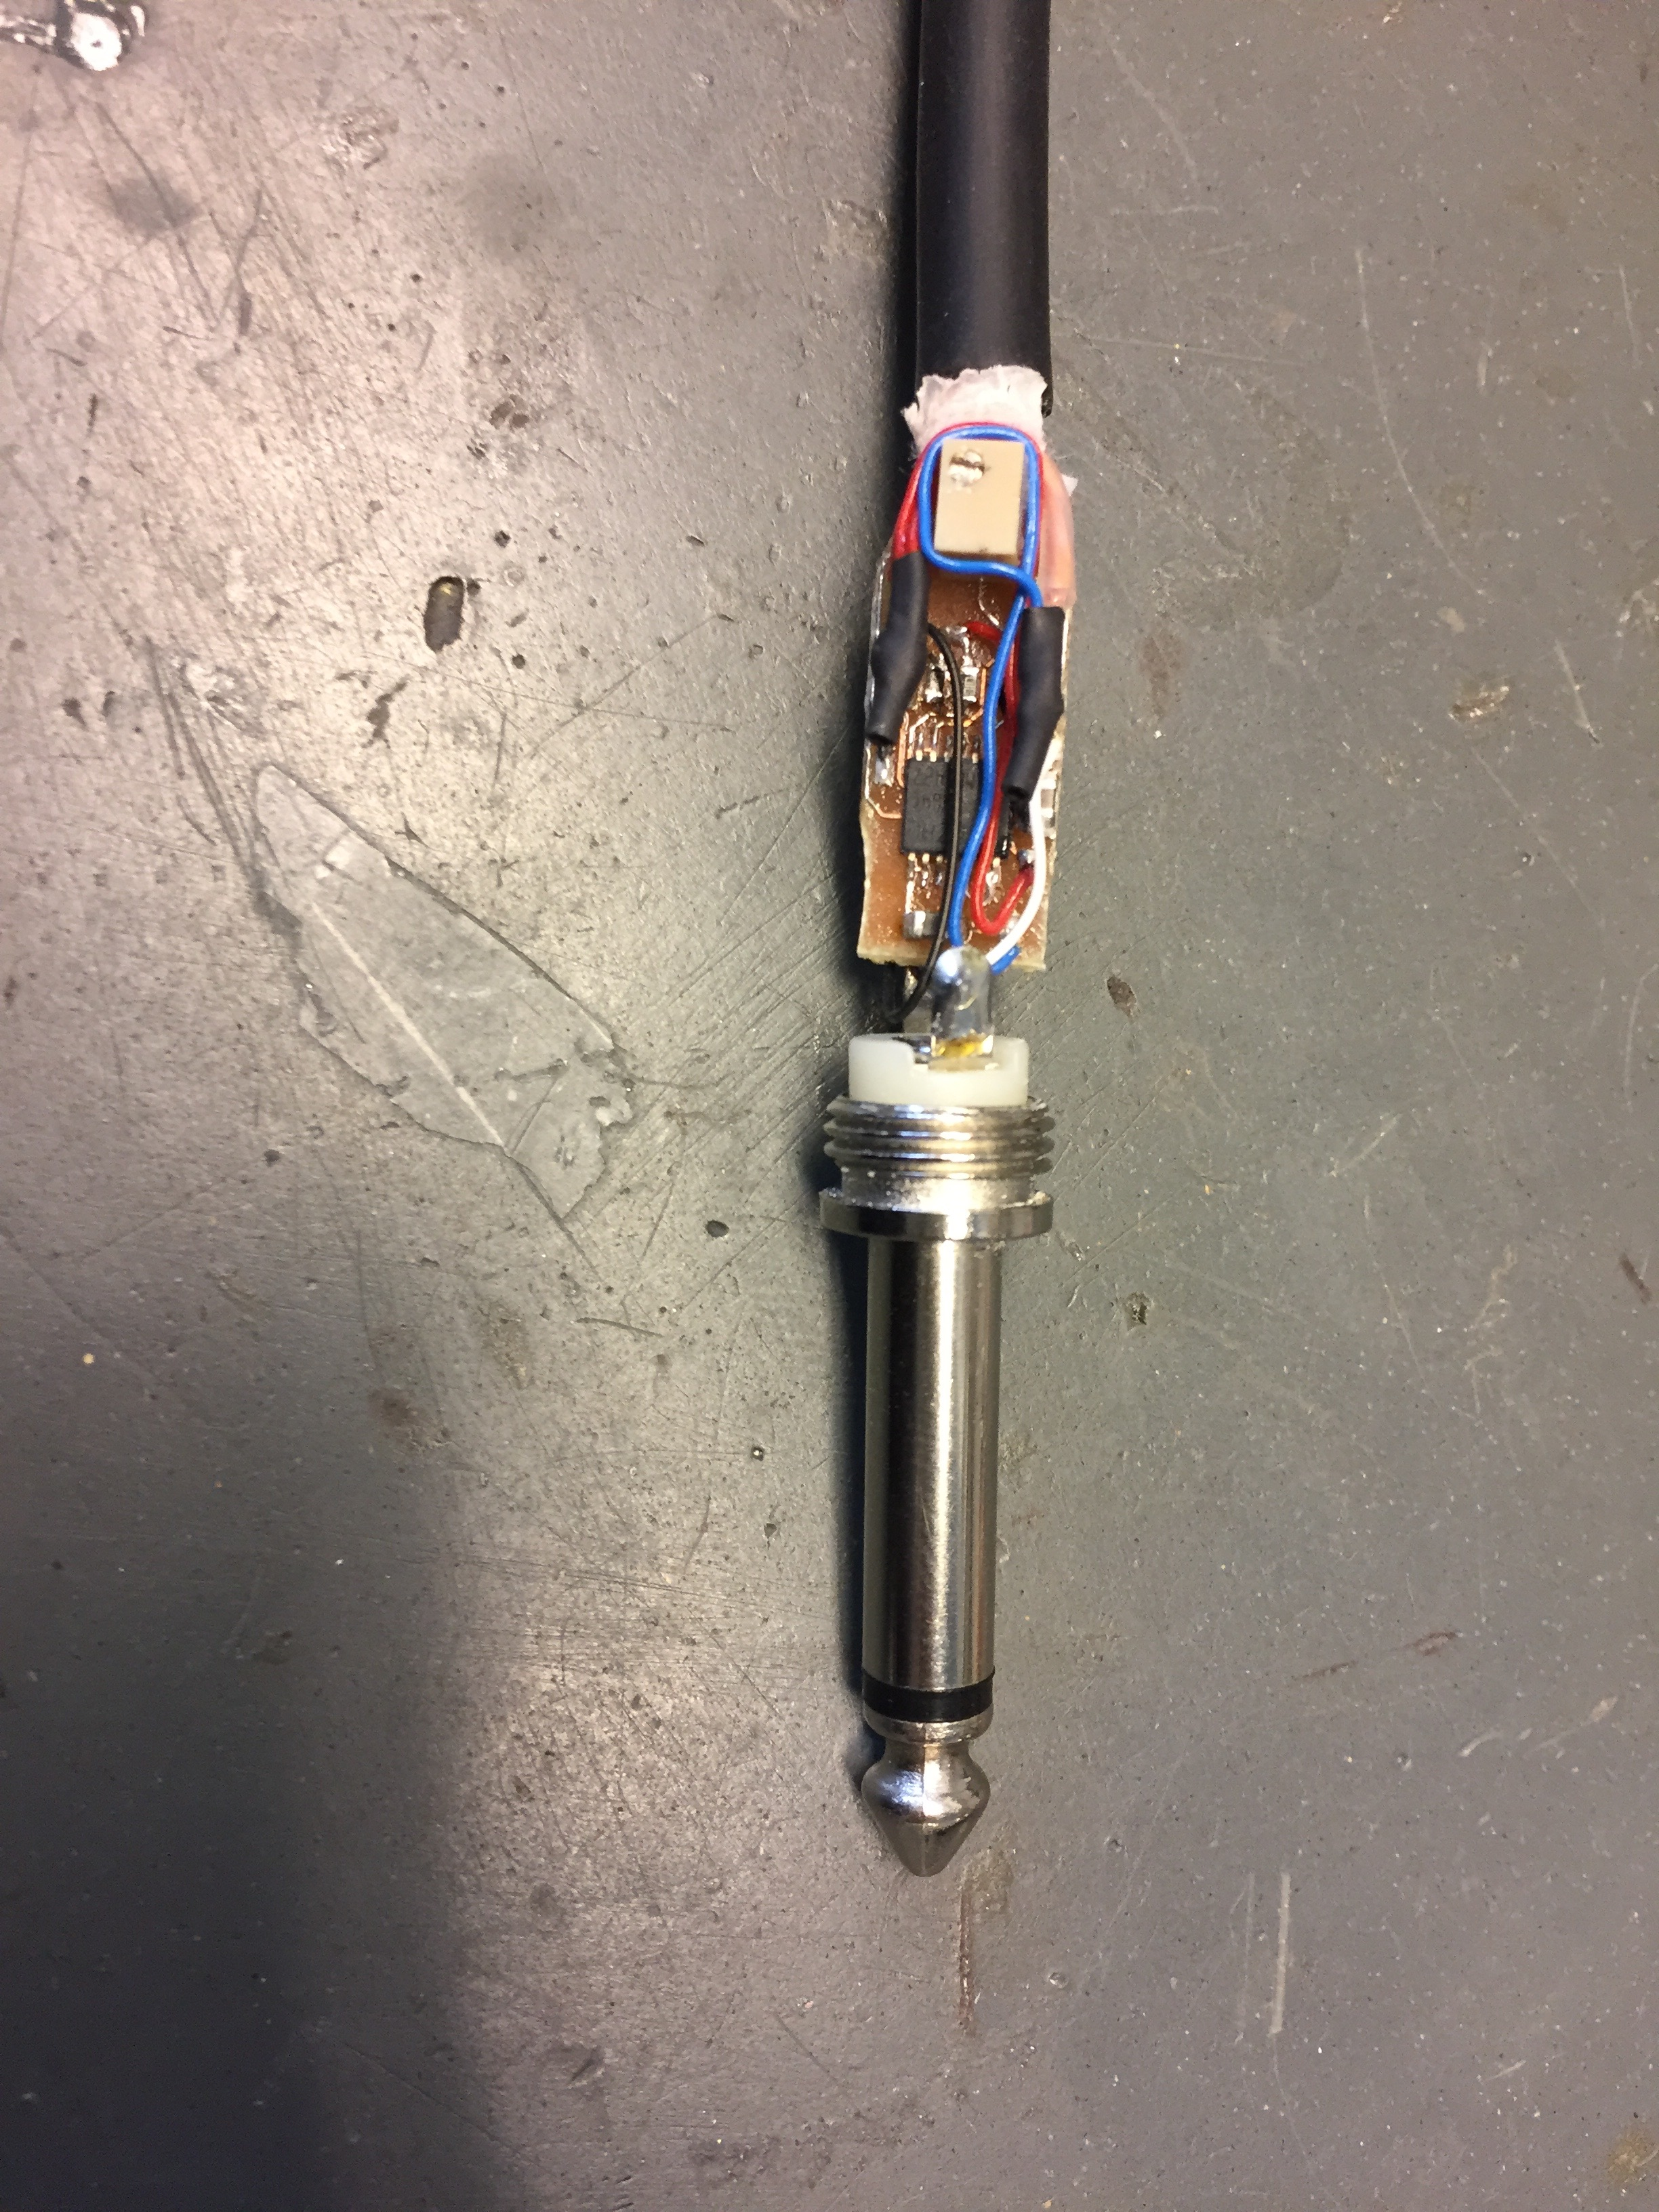
\includegraphics[width=\textwidth, angle=90]{preamp_pcb.jpg}
		\caption{The picture shows the mounted \gls{preamp} \gls{pcb} soldered to the jack connector}
		\label{fig:tests:preamp_pcb}
\end{subfigure}
 \qquad \qquad \qquad
\begin{subfigure}[htbp]{0.35\textwidth}
		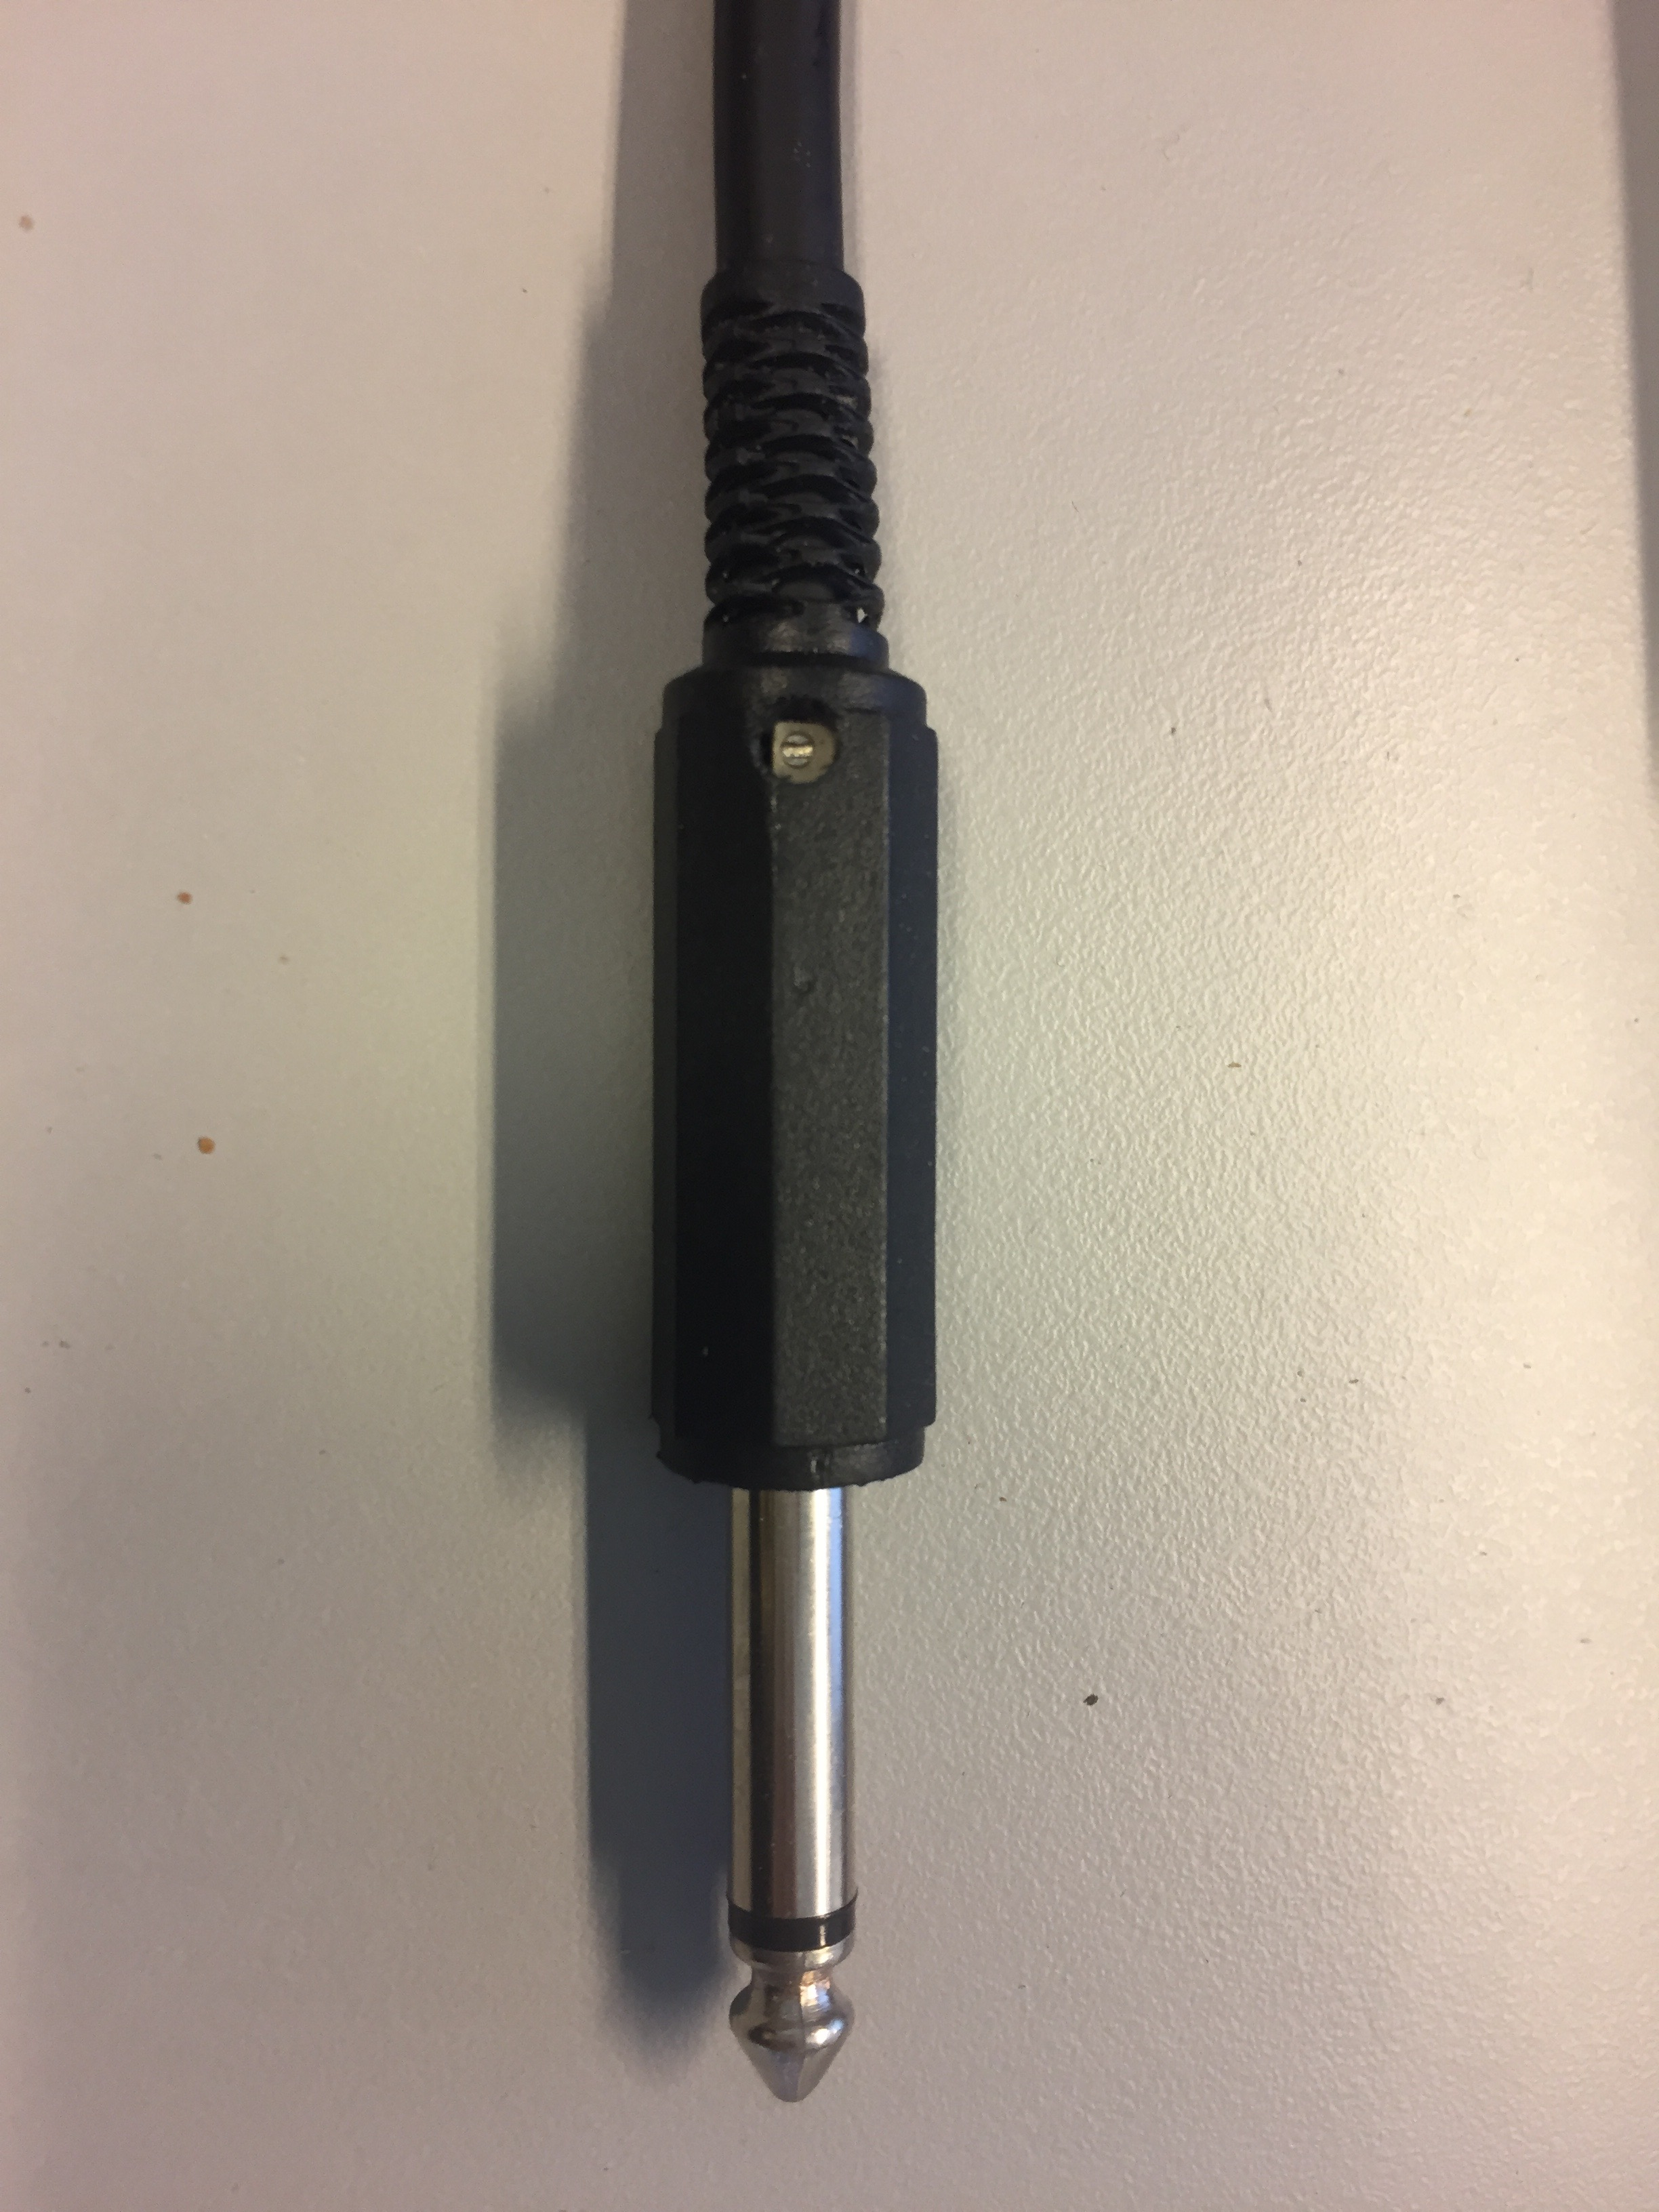
\includegraphics[width=\textwidth, angle=90]{preamp_jack.jpg}
		\caption{The picture shows the mounted \gls{preamp} \gls{pcb} inside the jack house.}
		\label{fig:tests:preamp_jack}
\end{subfigure} 
\caption{The \gls{preamp}}
\end{figure}

The \gls{preamp} \gls{pcb} fits inside the jack house, so \autoref{req:preamp5} and \autoref{req:preamp6} is approved.




\subsection{Test Review of the \gls{preamp}}
In this subsection, a short review will be shown of the \gls{preamp} test.

\begin{table}[H]
\centering
\caption{Recap of the requirements fulfilments for the \gls{preamp} test}
\label{test_of_preamp_table}
\begin{tabular}{|l|l|}
\hline
\rowcolor[HTML]{9B9B9B} 
\textbf{Requirement} & \textbf{Fulfilment State} \\ \hline
\textbf{\ref{req:preamp1}}    & \cmark                     \\ \hline
\textbf{\ref{req:preamp2}}    & \cmark                     \\ \hline
\textbf{\ref{req:preamp3}}    & \cmark                     \\ \hline
\textbf{\ref{req:preamp4}}    & \cmark                      \\ \hline
\textbf{\ref{req:preamp5}}    & \cmark                     \\ \hline
\textbf{\ref{req:preamp6}}    & \cmark                     \\ \hline
\end{tabular}
\end{table}


\newpage
\section{Test of the equalizer}
In this part, all the requirements related to the equalizer will be tested if they are fulfilled. 


\subsection{Test of \autoref{req:equalizer}}
According to \autoref{req:equalizer}, the gain value in each individual filter must be changeable by the user. This requirement has not been completely fulfilled since there has not been made an actual user interface for the effect. It is possible to change the gain of each individual filter, but only by writing it directly in the program. A test was made to prove this, where the peak filters with $\omega_0 =$ \SI{200}{\hertz} and $\omega_0 =$ \SI{3200}{\hertz} is set to amplify respectively \SI{6}{\decibel} and \SI{12}{\decibel}. 
\autoref{fig:tests:eq_gain} show the result of the test.

\begin{figure}[htbp!]
    \centering
        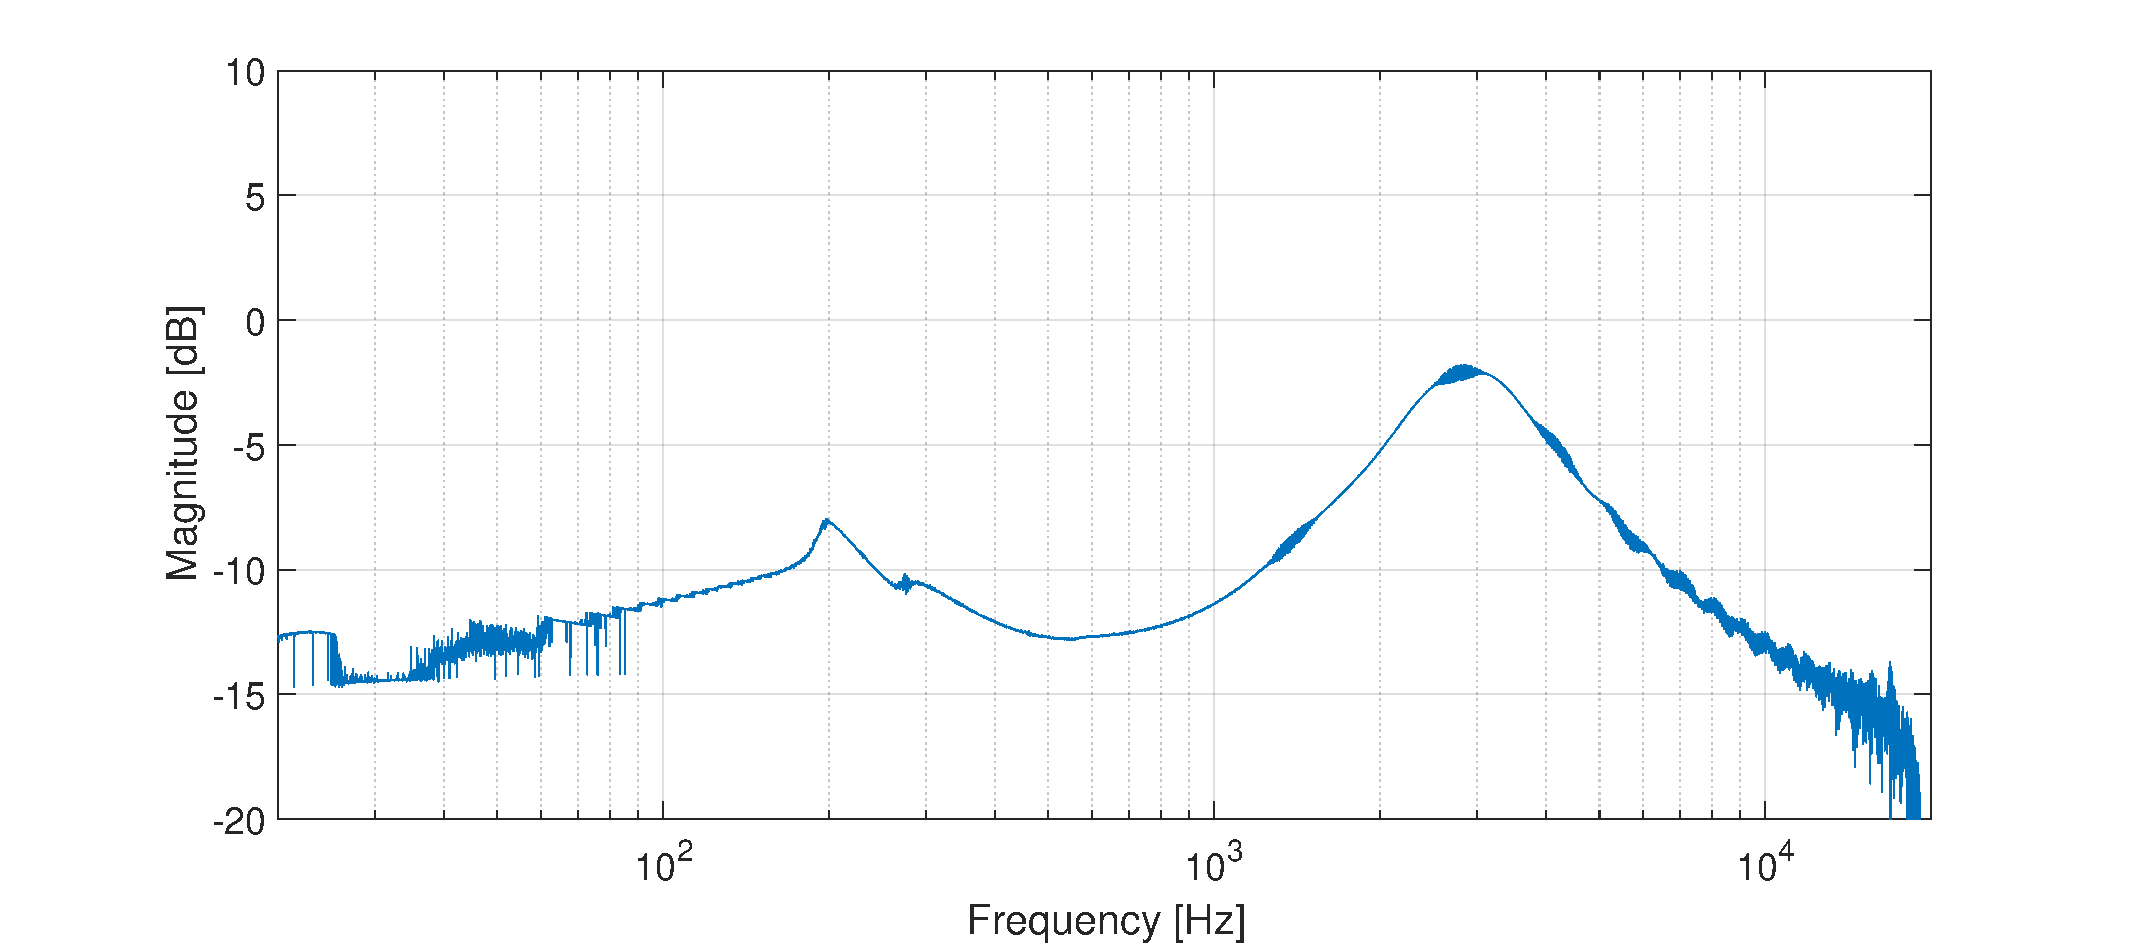
\includegraphics[width=\textwidth]{eq_200Hz_6db_3200Hz_12db.pdf}
        \caption{Measurement of the equalizer, where the peak filters with $\omega_0 =$ \SI{200}{\hertz} and $\omega_0 =$ \SI{3200}{\hertz} is set to amplify respectively \SI{6}{\decibel} and \SI{12}{\decibel}.}
        \label{fig:tests:eq_gain}
  \end{figure}



\subsection{Test of \autoref{req:equalizer2}}
According to \autoref{req:equalizer2}, each individual band must, when fully amplified, drop \SI{6}{\decibel} at the neighbouring center frequencies. A test was made using  the setup in \autoref{chap:effect_test_response}, where all the individual, fully amplified, filters and the combined filter, with all filters fully amplified, were tested. \autoref{fig:tests:eq_filters} shows the result of the test, where the upper blue graph is the combined equalizer and the others are the individual filters.

\begin{figure}[htbp!]
    \centering
        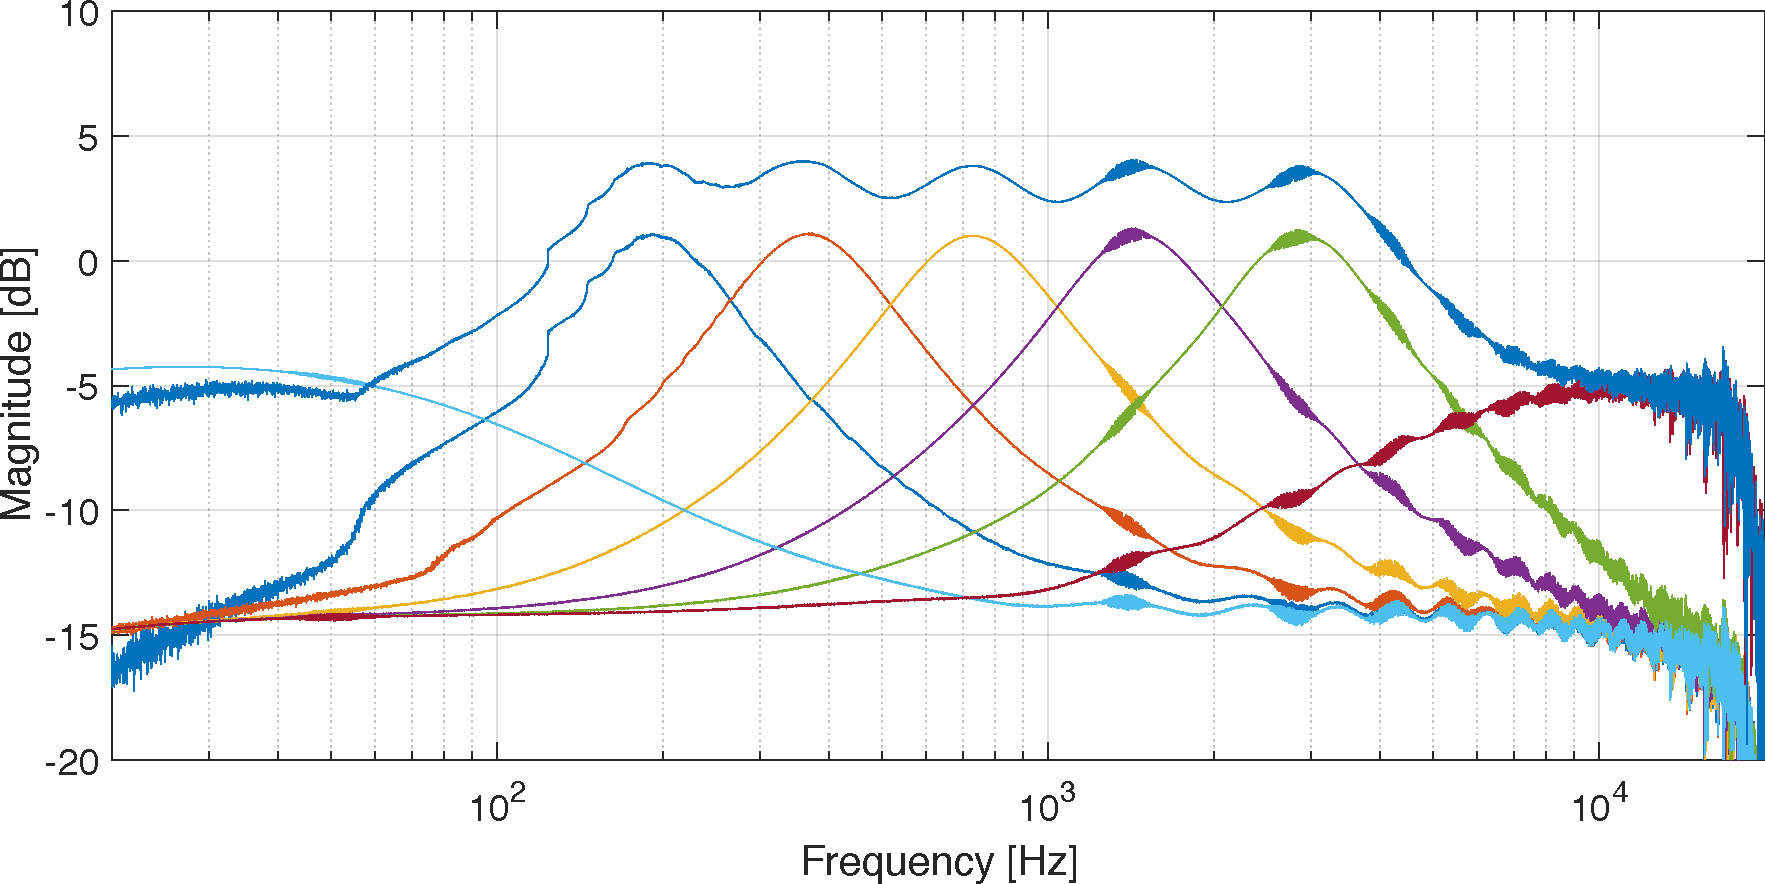
\includegraphics[width=\textwidth]{tested_eq.pdf}
        \caption{Measurement of the individual filters in the equalizer and the combined filter.}
        \label{fig:tests:eq_filters}
  \end{figure}
  
 In \autoref{fig:tests:eq_filters} it is seen that e.g. the peak filter with $\omega_0 =$ \SI{800}{\hertz} has dropped approximately \SI{6.5}{\decibel} at \SI{400}{\hertz} and \SI{1600}{\hertz}. It is also seen that at some frequencies, especially the high frequencies, the frequency response seems to oscillate. A measurement of the \gls{dsp}'s frequency response was made to investigate this. The result of the test i seen in \autoref{fig:tests:direct_dsp_gain}.

\begin{figure}[htbp!]
    \centering
        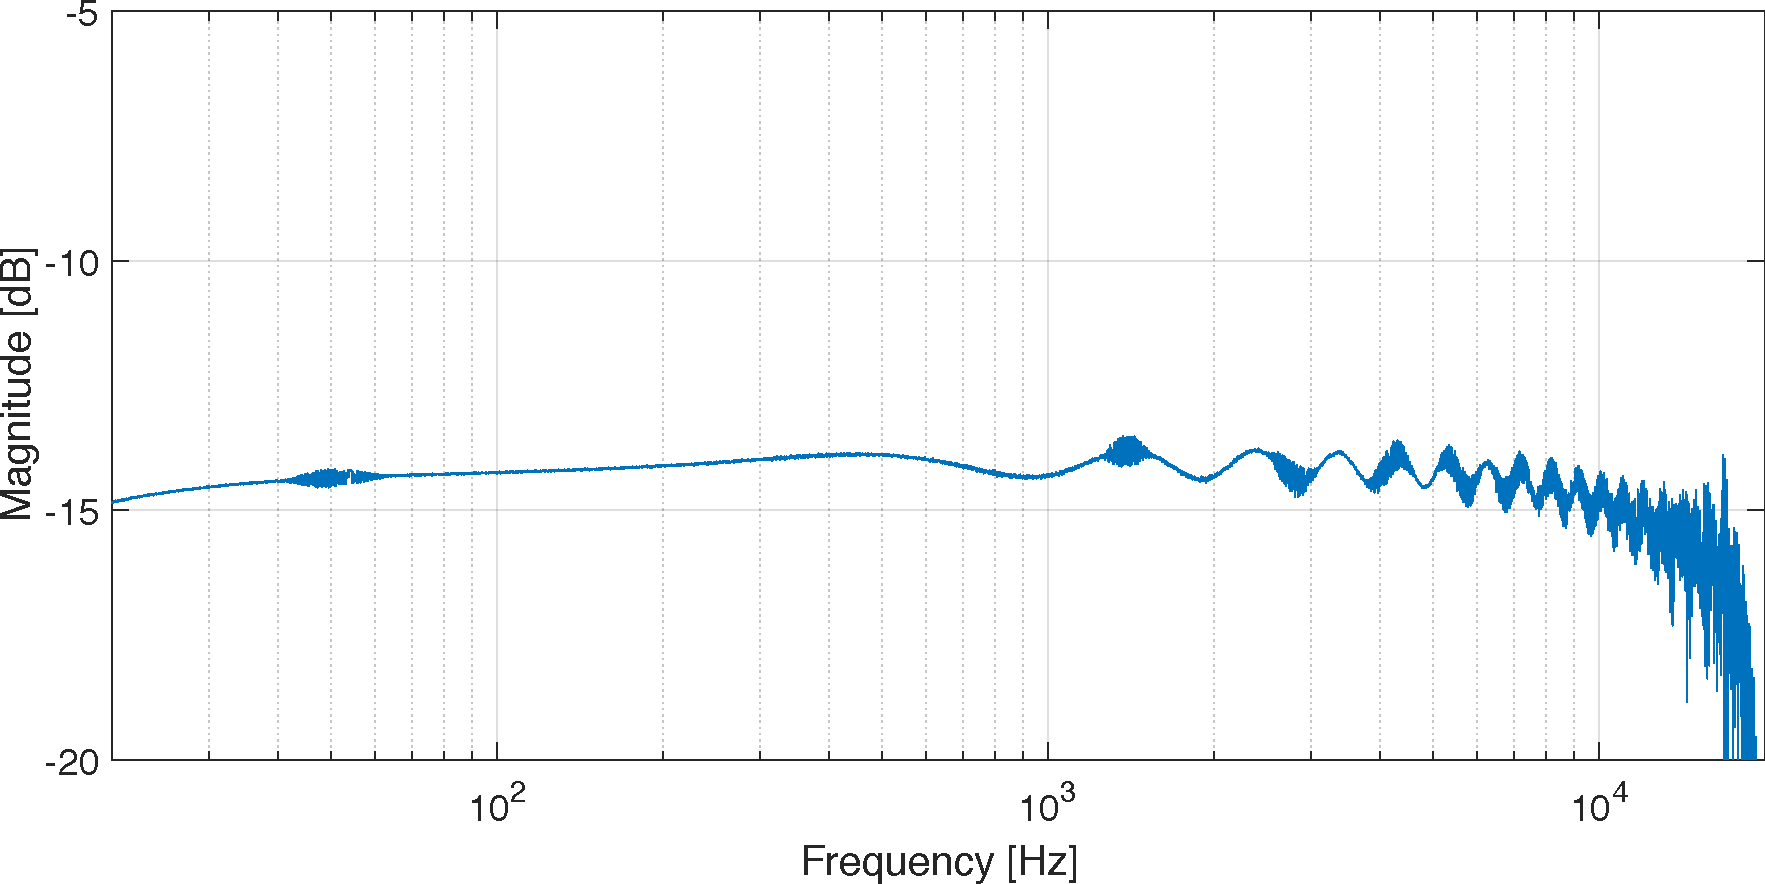
\includegraphics[width=\textwidth]{direct_dsp_gain.pdf}
        \caption{Measurement of the \gls{dsp}'s frequency response}
        \label{fig:tests:direct_dsp_gain}
  \end{figure}

\autoref{fig:tests:direct_dsp_gain} shows that the oscillations in \autoref{fig:tests:eq_filters} is because of the frequency response of the \gls{dsp}.
Thus the requirement is fulfilled. 

\subsection{Test review of the requirements for the equalizer}
In \autoref{tab:test_of_eq_table} the conclusion for the requirements related to the equalizer is summed.

\begin{table}[H]
\centering
\caption{Recap of the requirements fulfilments for the equalizer test}
\label{tab:test_of_eq_table}
\begin{tabular}{|l|l|}
\hline
\rowcolor[HTML]{9B9B9B} 
\textbf{Requirement} & \textbf{Fulfilment State} \\ \hline
\textbf{\ref{req:equalizer}}    & \cmark *                     \\ \hline
\textbf{\ref{req:equalizer2}}    & \cmark                      \\ \hline

\end{tabular}
\end{table}





 
%%
\part{Conclusion and discussion}\label{pt:conclusions}
\section{Conclusion}\label{sec:conclusion}

In the analysis \autoref{ch:analysing}, some initial problems were answered, regarding how the sound from an electric guitar could be personalized. It was found that a way to personalize the sound was by sending the signal through guitar effects, and it was found that by making the effects digitally, certain advantages followed. The following problem statement was made from this research:

\textbf{How can a number of digital guitar effects be designed and implemented using Digital Signal Processing?} \\

24 requirements were made for the further development of the product. 
It was found that the use of a \gls{dsp} was an ideal choice for implementing digital guitar effects. A \gls{preamp} was designed and constructed to connect the guitar and the \gls{dsp}, the \gls{dsp} was explained, and the initial setup of the \gls{dsp} was made. The five effects; the equalizer, \gls{reverb}, delay, chorus and flanger where designed, and the three effects; the equalizer, \gls{reverb} and flanger were implemented on the \gls{dsp} using asembly.
The final system were tested and held against the stated requirements. \\

It can be concluded that parts of the equalizer, the \gls{reverb} and the flanger could be implemented digitally on a \gls{dsp}.  


 
%

\glsresetall
\appendix % Start of appendix
\addtocontents{toc}{\protect\setcounter{tocdepth}{0}} 
%\input{chapters/appendices/_appendices} % Include appendices
%Appendix:

 \graphicspath{{figures/appendix/}}
\part{Appendix}\label{pt:appendix}
\chapter{Test a guitars frequency area}\label{app:frequency_area}
A test was made to get a view of the frequency area, in which the tones from a guitar lies.

\section*{Materials and setup}
To measure the frequency area on a guitar, the following materials are used:
\begin{itemize}
\item Digilent Analog Discovery 2 (Oscilloscope)
\item Fender Squier Classic Vibe Telecaster (Guitar)
\item Digilent Waveforms 2015 (PC - software)
\end{itemize}

\begin{figure}[htbp!]
\centering
\def\svgwidth{\columnwidth}
\chapter{Test a guitars frequency area}\label{app:frequency_area}
A test was made to get a view of the frequency area, in which the tones from a guitar lies.

\section*{Materials and setup}
To measure the frequency area on a guitar, the following materials are used:
\begin{itemize}
\item Digilent Analog Discovery 2 (Oscilloscope)
\item Fender Squier Classic Vibe Telecaster (Guitar)
\item Digilent Waveforms 2015 (PC - software)
\end{itemize}

\begin{figure}[htbp!]
\centering
\def\svgwidth{\columnwidth}
\input{figures/appendix/guitar_frequency_test.pdf_tex}
\caption{Setup for measuring frequency area on a guitar.}
		\label{fig:appendix:guitar_freq}
\end{figure}

\section*{Test procedure}
To the frequency area on a guitar, the following steps are made:
\begin{enumerate}
\item The materials are set up as in \autoref{fig:appendix:guitar_freq}.
\item Digilent Waveforms 2015 is set as a spectrum analyser. 
\item The guitar is set to use the neck pickup and the volume control and the tone control are turned all the way up.
\item The highest and the lowest tone on the guitar are played, measured by the oscilloscope and analysed in Digilent Waveforms 2015.
\item The guitar is set to use the bridge pickup and step 4 is repeated. 
\item The data is plotted in MATLAB.
\end{enumerate}

\section*{Results}

\begin{figure}[htbp!]
	\centering
		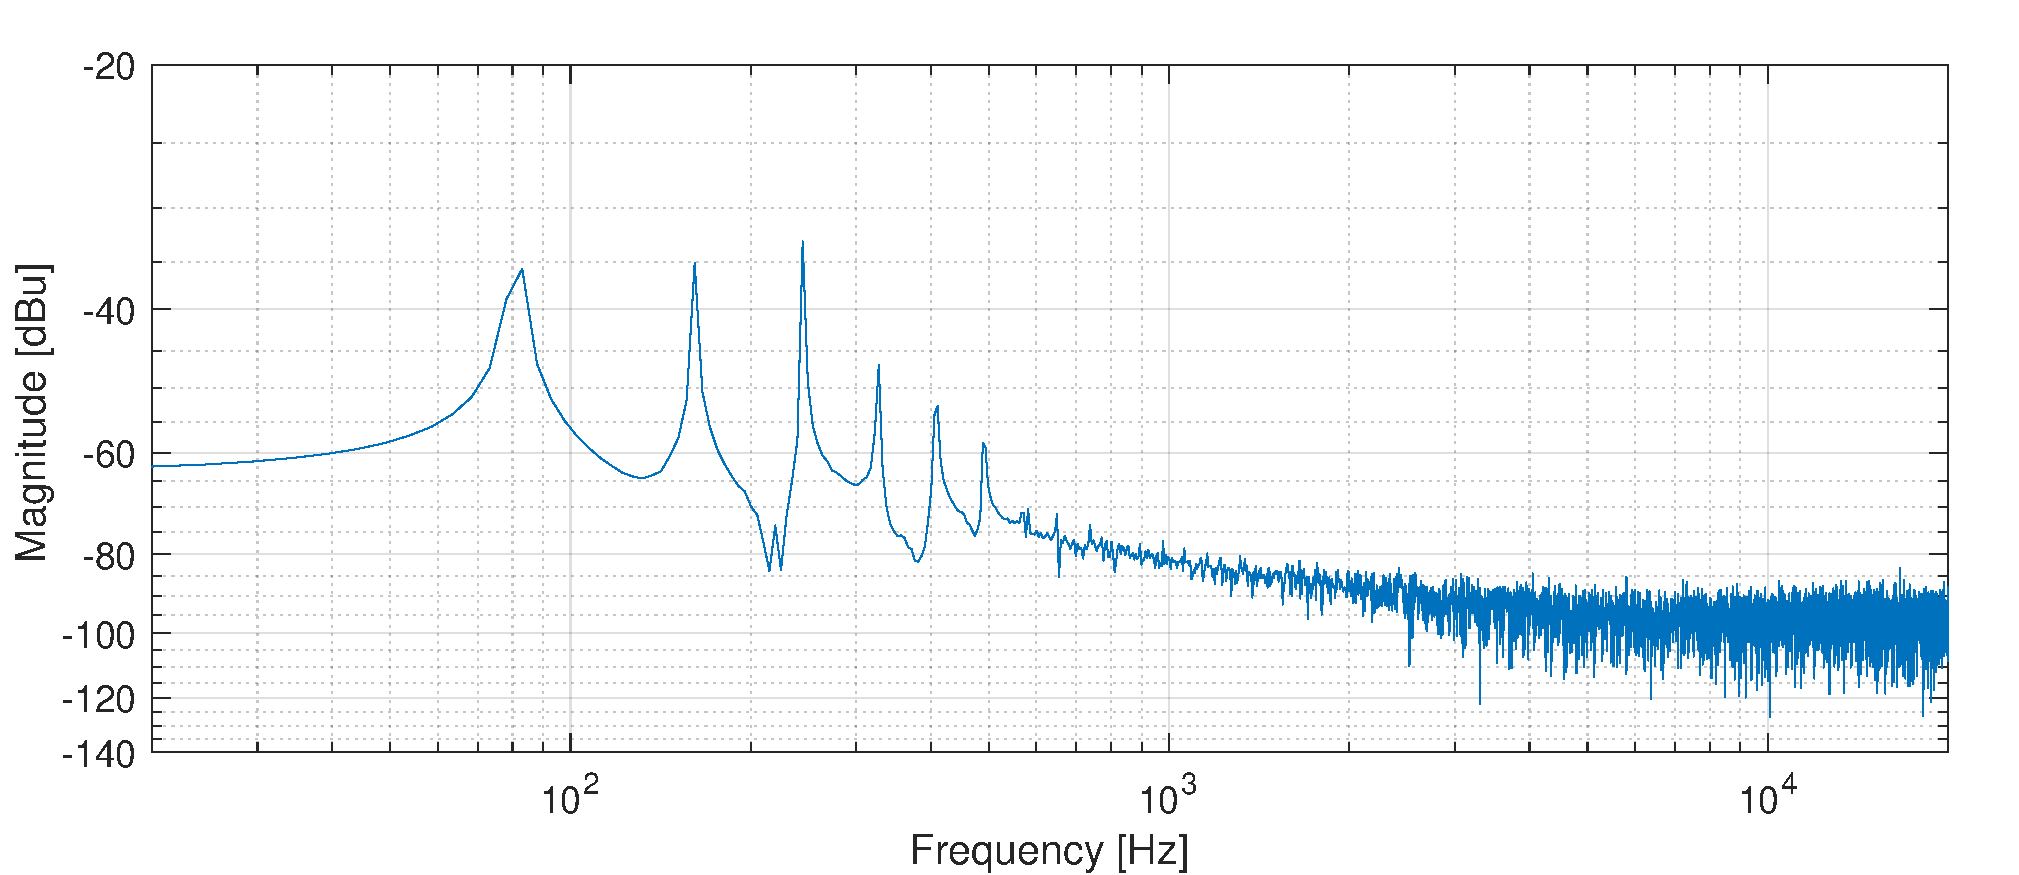
\includegraphics[width=1\textwidth]{guitar_low_E_neck.pdf}
		\caption{Measurement of the low E note on the neck pickup.}
		\label{fig:appendix:low_E_neck}
\end{figure}

On  \autoref{fig:appendix:low_E_neck} it is seen that the lowest significant frequency is around \SI{80}{\hertz} and the highest significant frequency is around \SI{400}{\hertz}, when playing the low E note on the guitar, using the neck pickup.

\begin{figure}[htbp!]
	\centering
		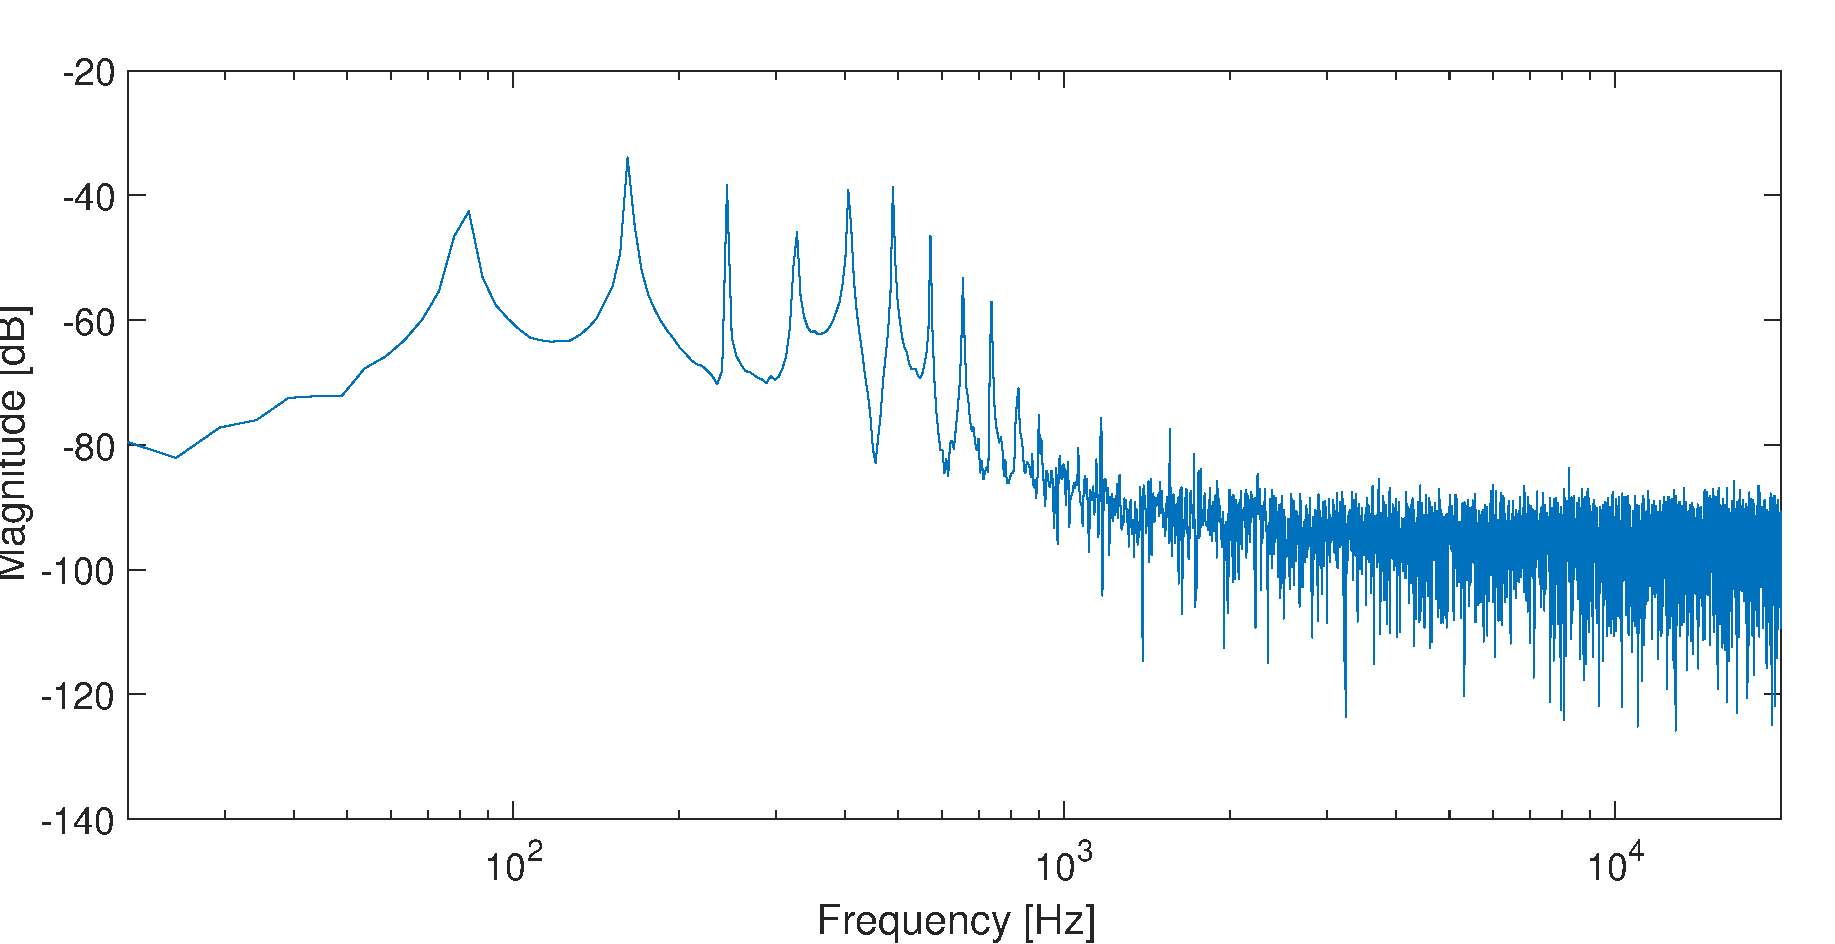
\includegraphics[width=1\textwidth]{guitar_low_E_bridge.pdf}
		\caption{Measurement of the low E note on the bridge pickup.}
		\label{fig:appendix:low_E_bridge}
\end{figure}

On  \autoref{fig:appendix:low_E_bridge} it is seen that the lowest significant frequency is around \SI{80}{\hertz} and the highest significant frequency is around \SI{730}{\hertz}, when playing the low E note on the guitar, using the bridge pickup.

\begin{figure}[htbp!]
	\centering
		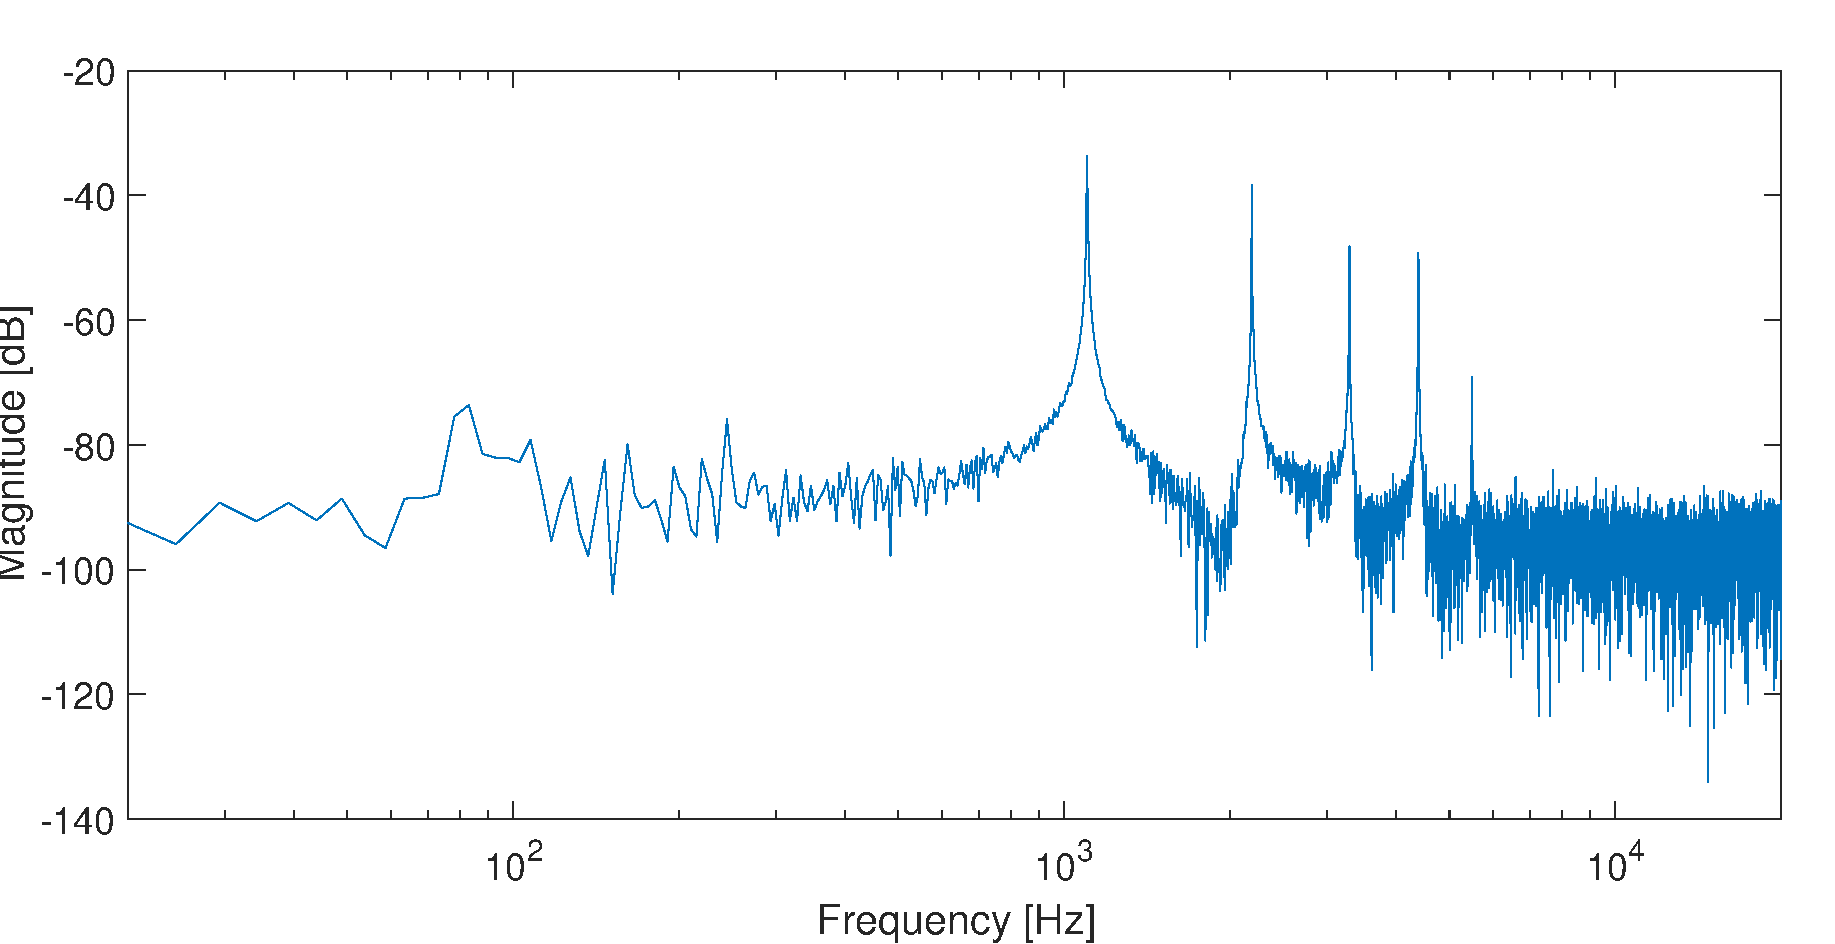
\includegraphics[width=1\textwidth]{guitar_high_Cis_neck.pdf}
		\caption{Measurement of the high C\# note on the neck pickup.}
		\label{fig:appendix:high_Cis_neck}
\end{figure}

On  \autoref{fig:appendix:high_Cis_neck} it is seen that the lowest significant frequency is around \SI{1100}{\hertz} and the highest significant frequency is around \SI{4400}{\hertz}, when playing the high C\# note on the guitar, using the neck pickup.

\begin{figure}[htbp!]
	\centering
		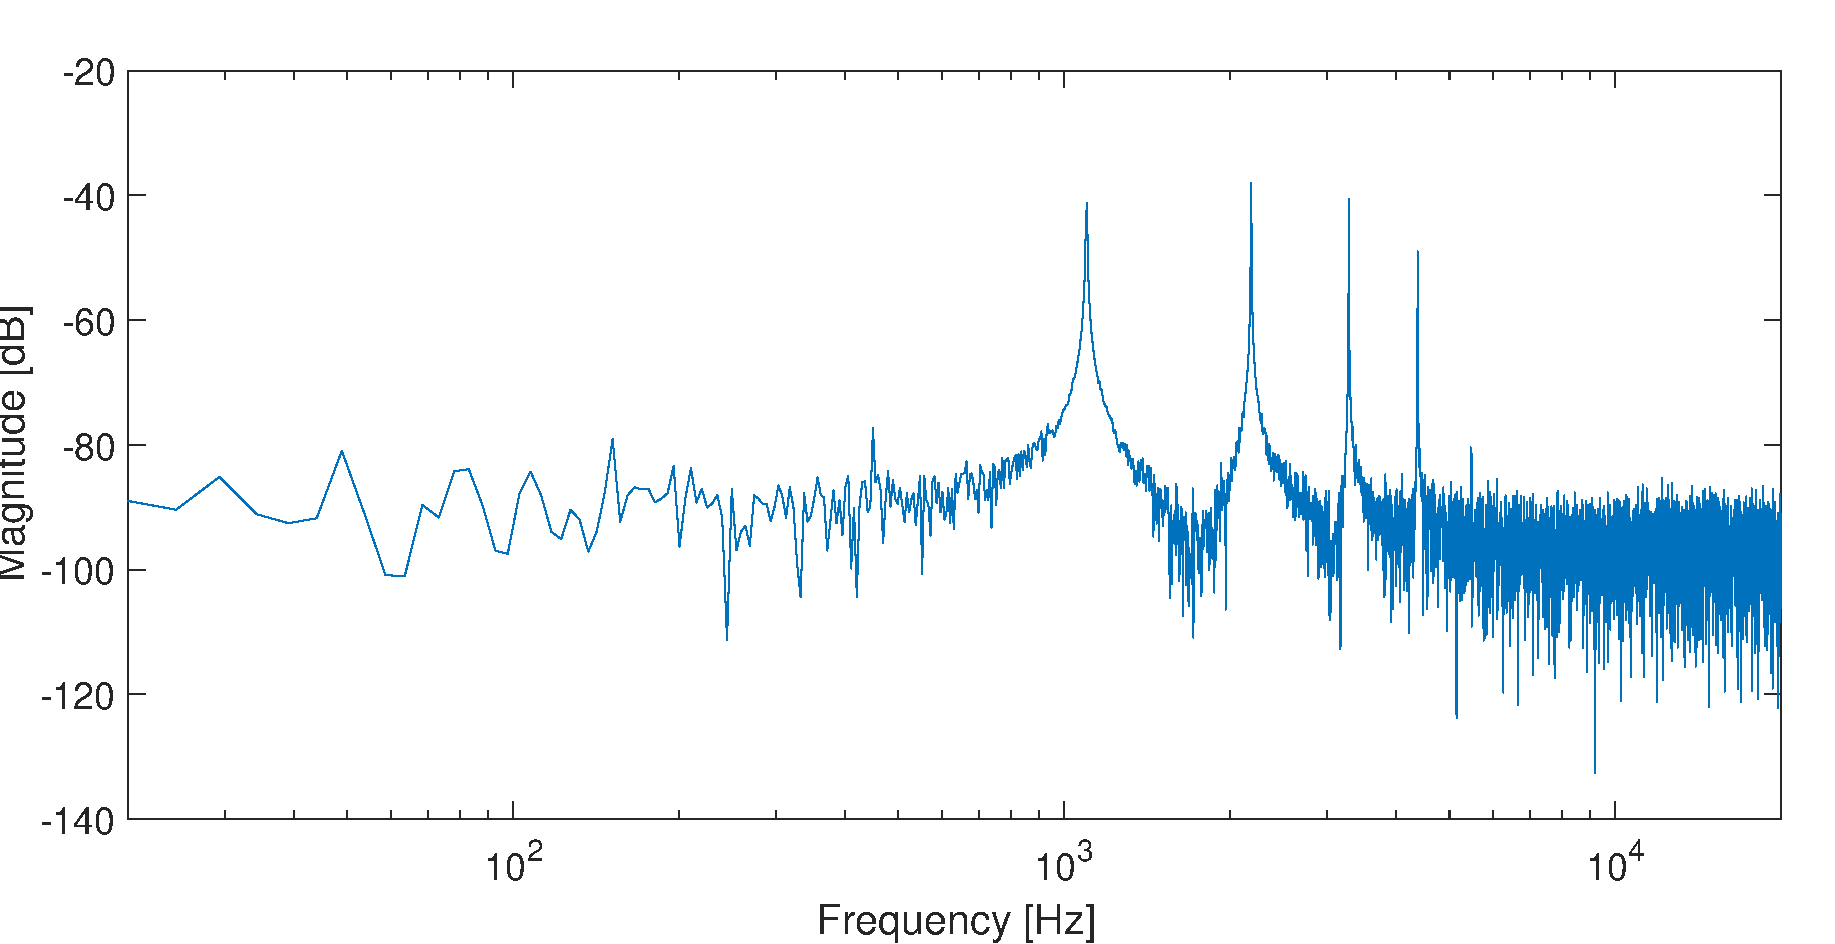
\includegraphics[width=1\textwidth]{guitar_high_Cis_bridge.pdf}
		\caption{Measurement of the high C\# note on the bridge pickup.}
		\label{fig:appendix:high_Cis_bridge}
\end{figure}

On  \autoref{fig:appendix:high_Cis_bridge} it is seen that the lowest significant frequency is around \SI{1100}{\hertz} and the highest significant frequency is around \SI{4400}{\hertz}, when playing the high C\# note on the guitar, using the bridge pickup. 

\begin{figure}[htbp!]
	\centering
		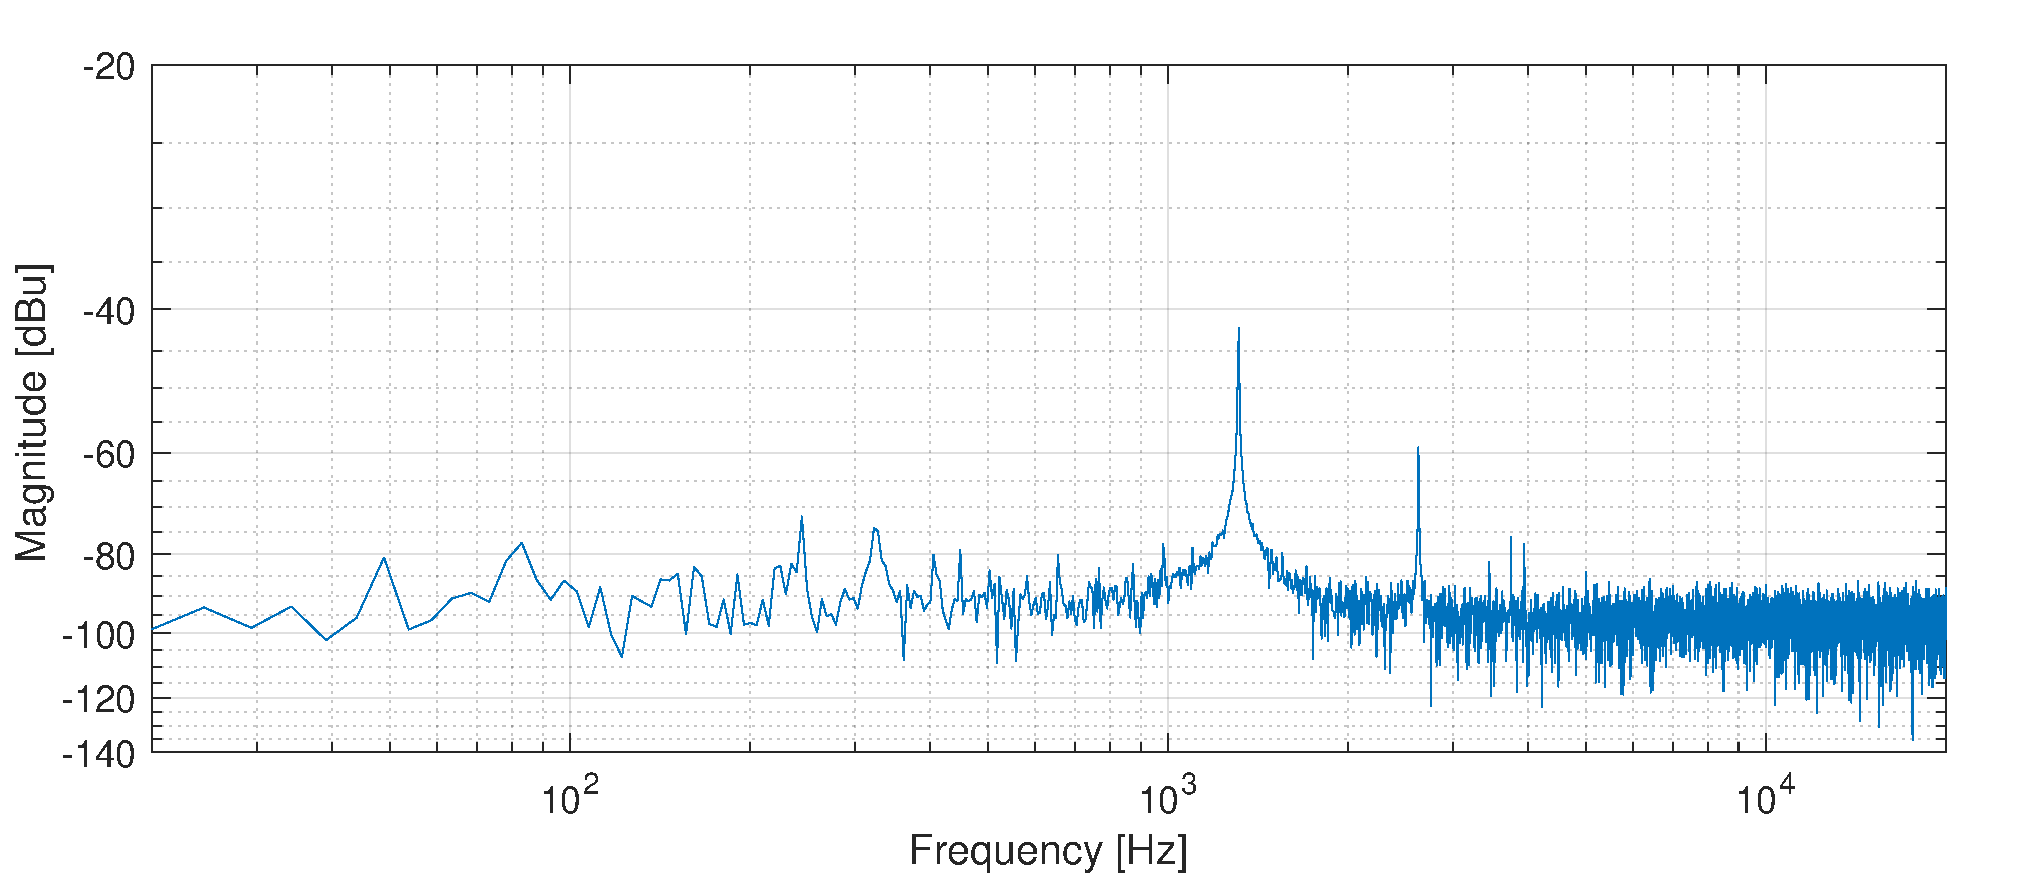
\includegraphics[width=1\textwidth]{guitar_high_E_flasholet_bridge.pdf}
		\caption{Measurement of the high E note, played as flasholet, on the bridge pickup.}
		\label{fig:appendix:high_E_bridge_flasholet}
\end{figure}

On  \autoref{fig:appendix:high_E_bridge_flasholet} it is seen that the lowest significant frequency is around \SI{1300}{\hertz} and the highest significant frequency is around \SI{2600}{\hertz}, when playing the high E note on the guitar as flasholet, using the bridge pickup. 

\caption{Setup for measuring frequency area on a guitar.}
		\label{fig:appendix:guitar_freq}
\end{figure}

\section*{Test procedure}
To the frequency area on a guitar, the following steps are made:
\begin{enumerate}
\item The materials are set up as in \autoref{fig:appendix:guitar_freq}.
\item Digilent Waveforms 2015 is set as a spectrum analyser. 
\item The guitar is set to use the neck pickup and the volume control and the tone control are turned all the way up.
\item The highest and the lowest tone on the guitar are played, measured by the oscilloscope and analysed in Digilent Waveforms 2015.
\item The guitar is set to use the bridge pickup and step 4 is repeated. 
\item The data is plotted in MATLAB.
\end{enumerate}

\section*{Results}

\begin{figure}[htbp!]
	\centering
		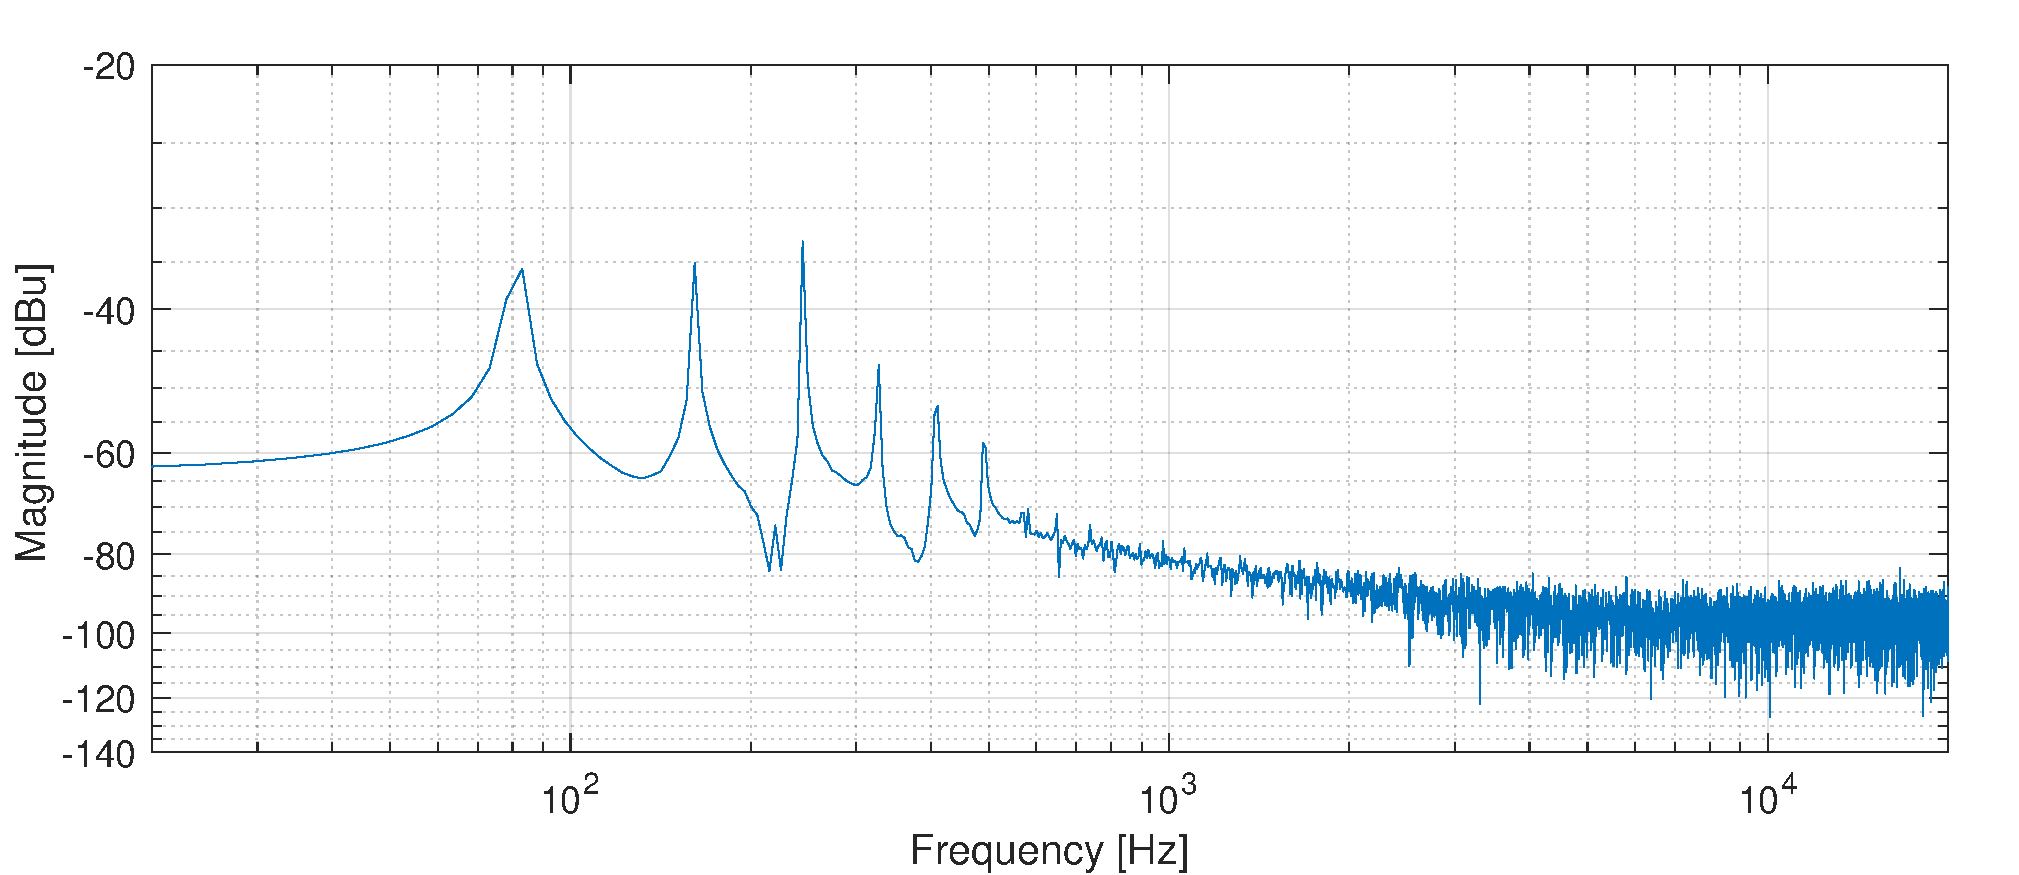
\includegraphics[width=1\textwidth]{guitar_low_E_neck.pdf}
		\caption{Measurement of the low E note on the neck pickup.}
		\label{fig:appendix:low_E_neck}
\end{figure}

On  \autoref{fig:appendix:low_E_neck} it is seen that the lowest significant frequency is around \SI{80}{\hertz} and the highest significant frequency is around \SI{400}{\hertz}, when playing the low E note on the guitar, using the neck pickup.

\begin{figure}[htbp!]
	\centering
		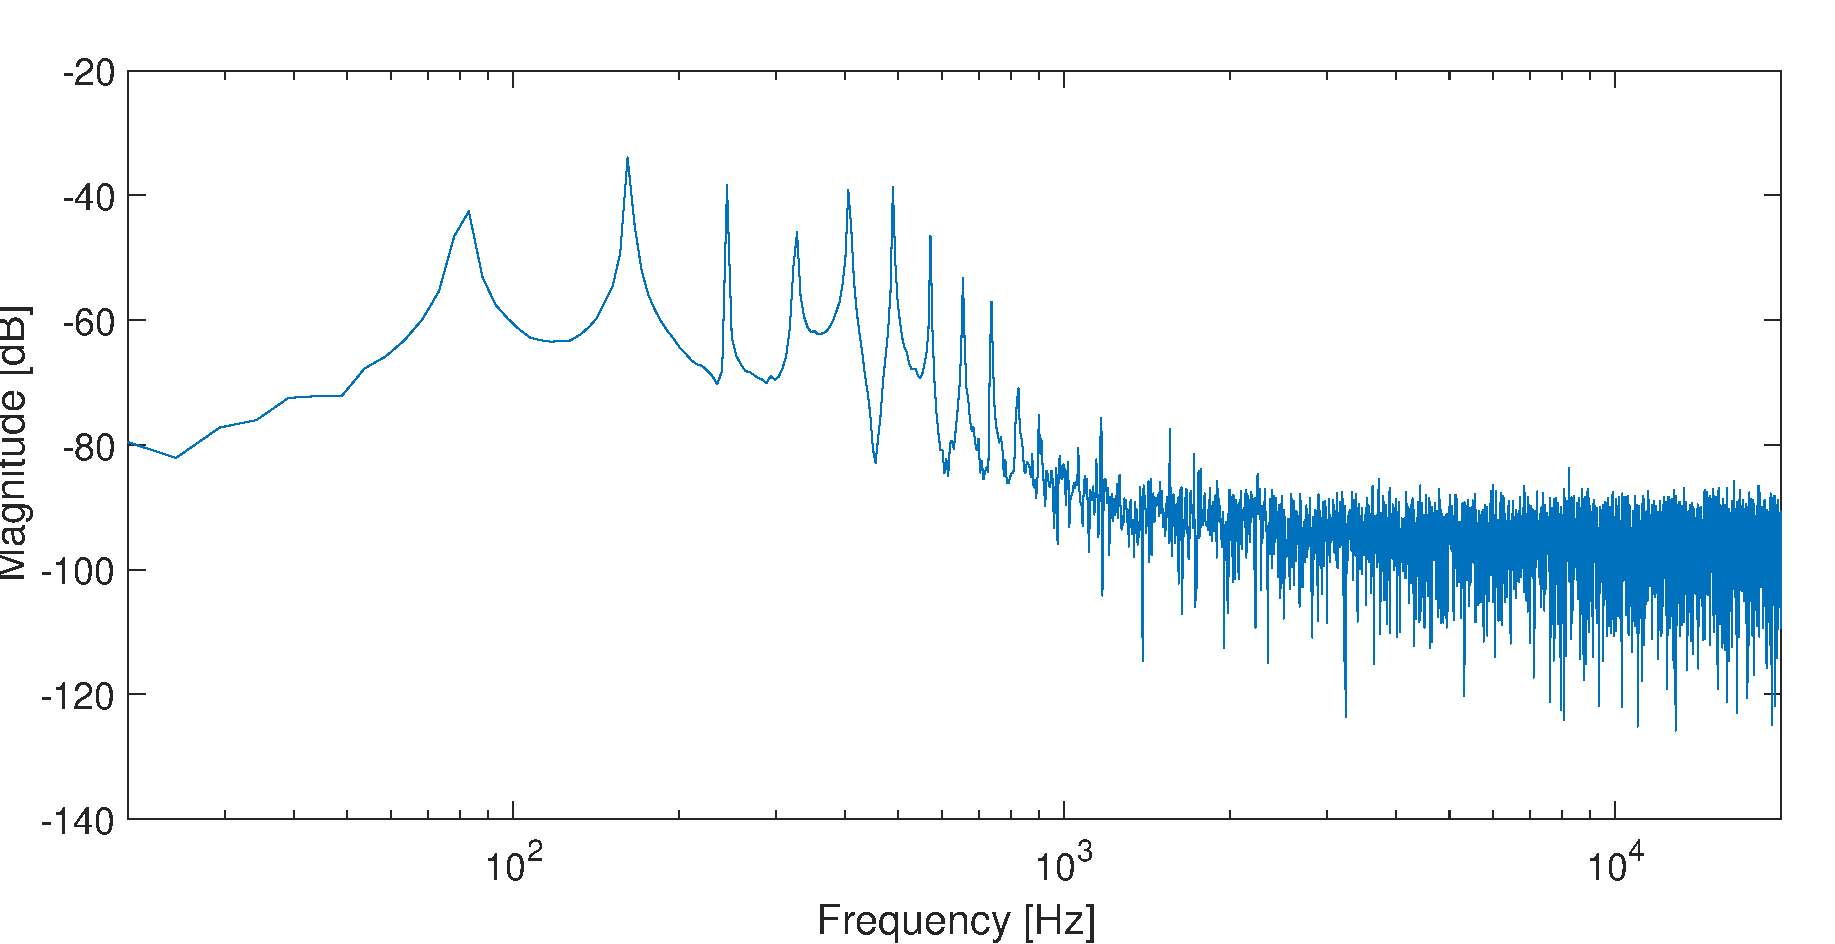
\includegraphics[width=1\textwidth]{guitar_low_E_bridge.pdf}
		\caption{Measurement of the low E note on the bridge pickup.}
		\label{fig:appendix:low_E_bridge}
\end{figure}

On  \autoref{fig:appendix:low_E_bridge} it is seen that the lowest significant frequency is around \SI{80}{\hertz} and the highest significant frequency is around \SI{730}{\hertz}, when playing the low E note on the guitar, using the bridge pickup.

\begin{figure}[htbp!]
	\centering
		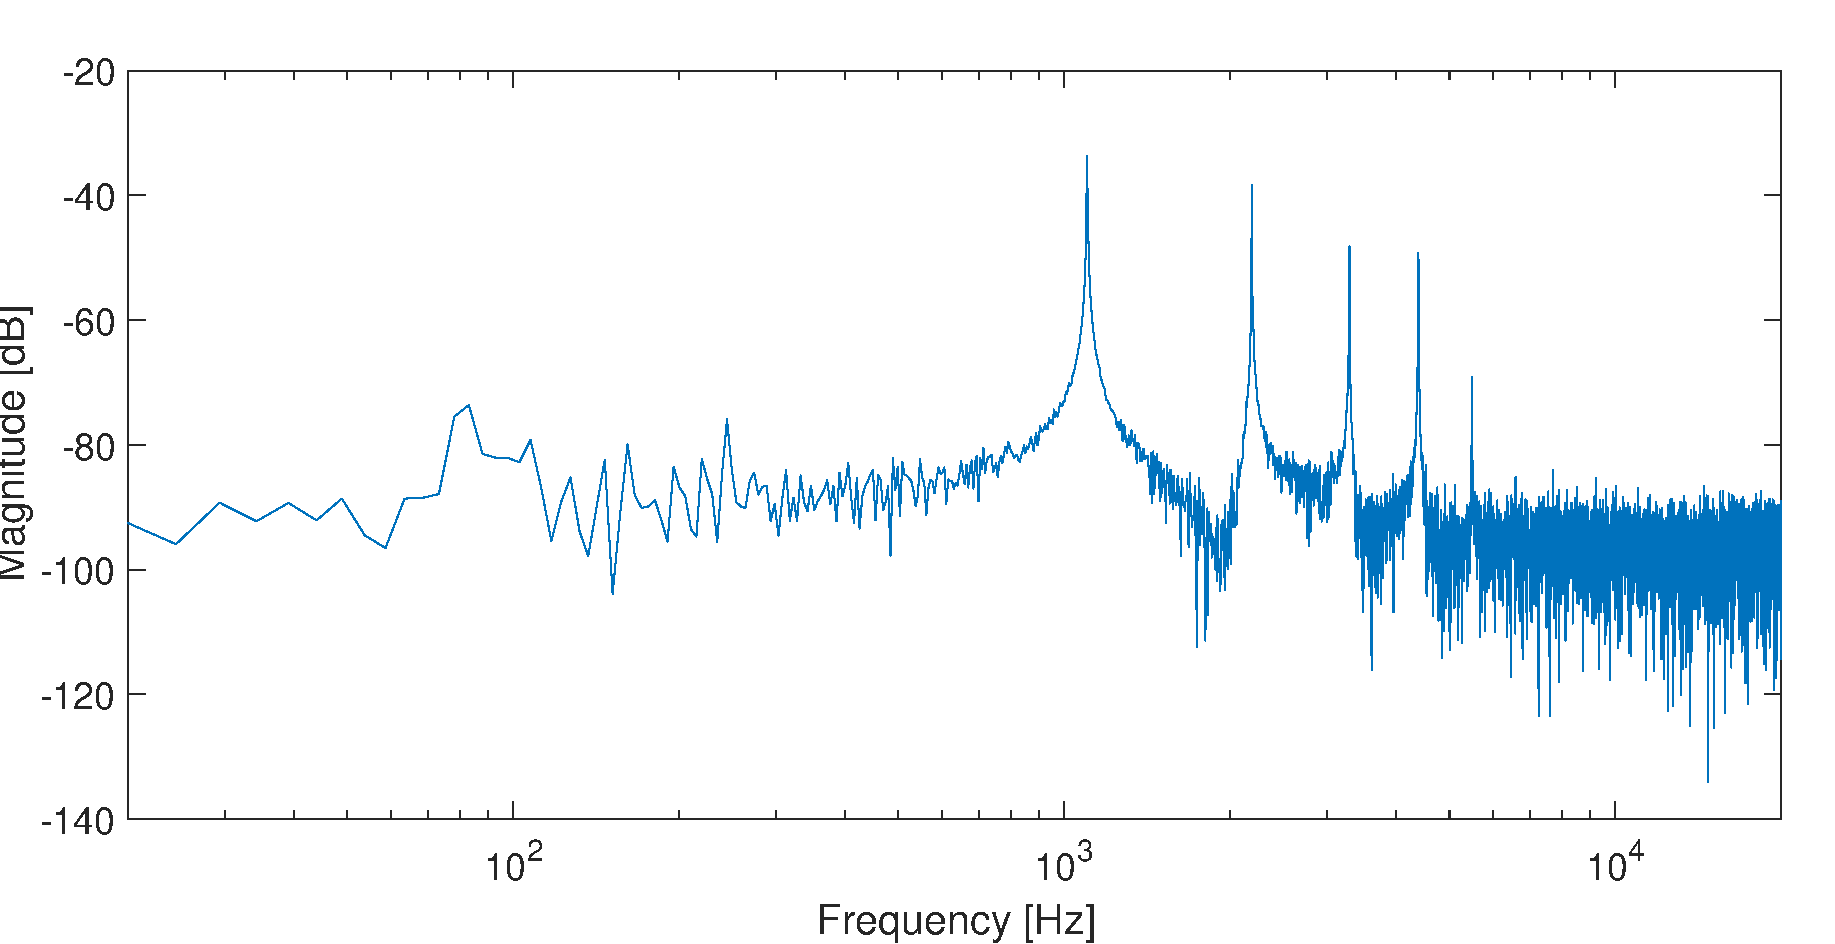
\includegraphics[width=1\textwidth]{guitar_high_Cis_neck.pdf}
		\caption{Measurement of the high C\# note on the neck pickup.}
		\label{fig:appendix:high_Cis_neck}
\end{figure}

On  \autoref{fig:appendix:high_Cis_neck} it is seen that the lowest significant frequency is around \SI{1100}{\hertz} and the highest significant frequency is around \SI{4400}{\hertz}, when playing the high C\# note on the guitar, using the neck pickup.

\begin{figure}[htbp!]
	\centering
		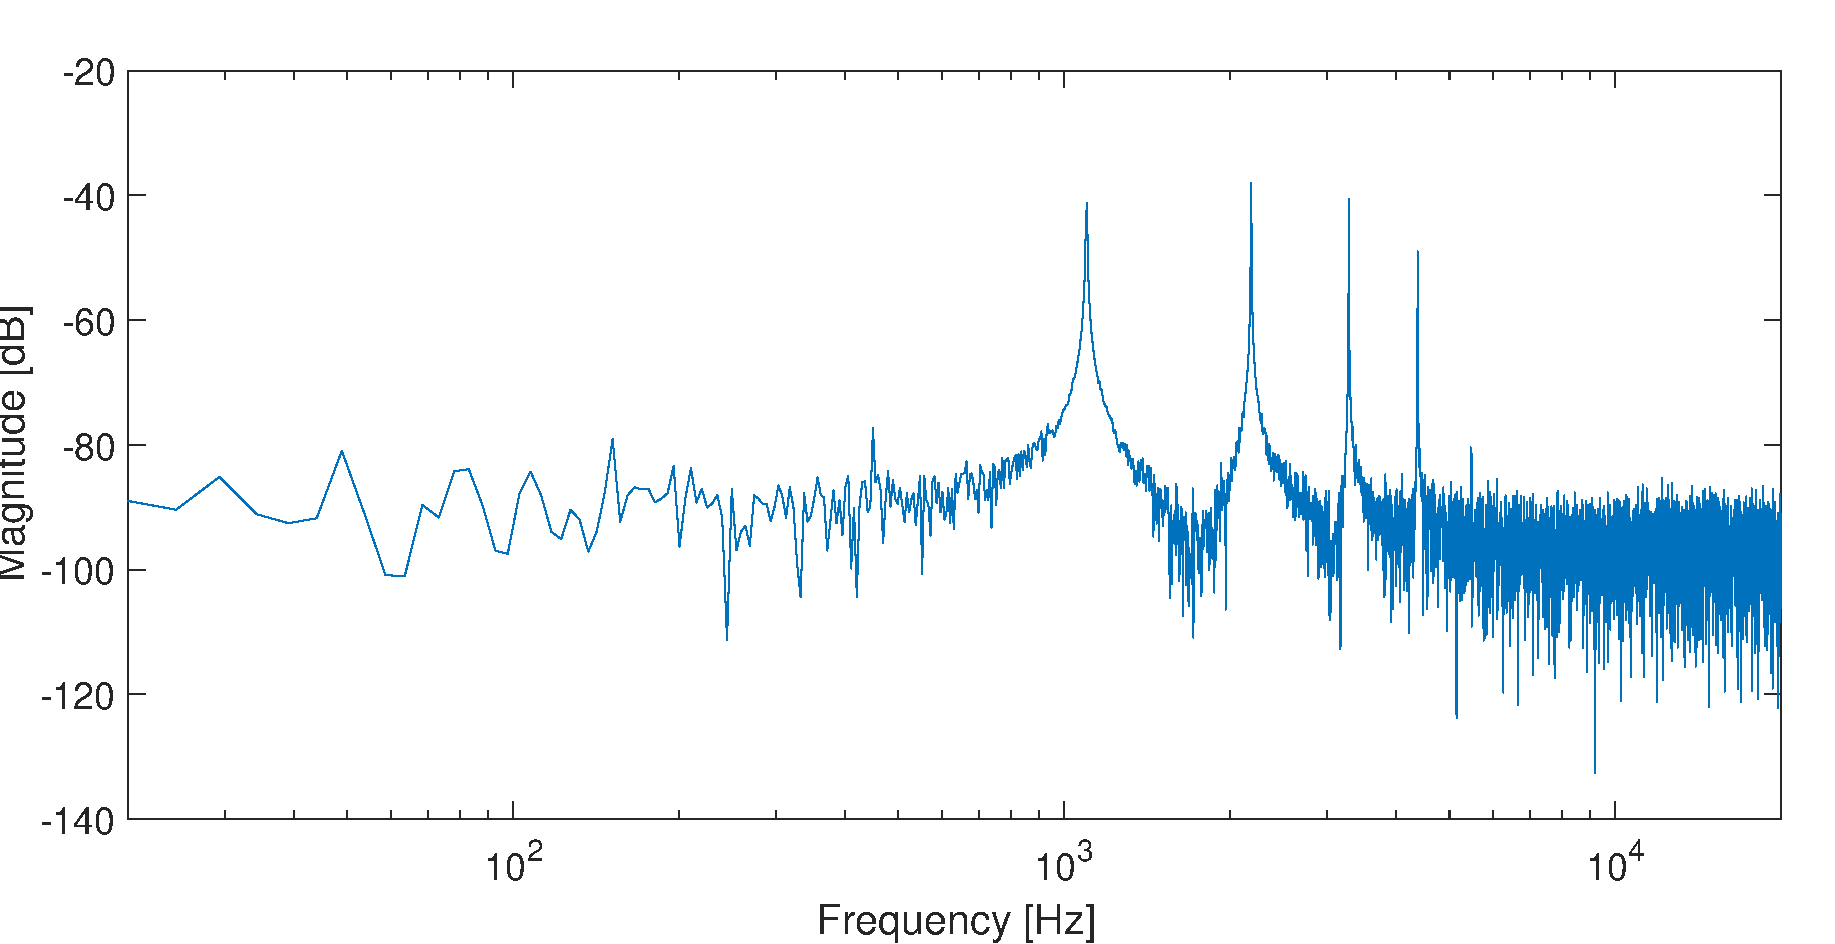
\includegraphics[width=1\textwidth]{guitar_high_Cis_bridge.pdf}
		\caption{Measurement of the high C\# note on the bridge pickup.}
		\label{fig:appendix:high_Cis_bridge}
\end{figure}

On  \autoref{fig:appendix:high_Cis_bridge} it is seen that the lowest significant frequency is around \SI{1100}{\hertz} and the highest significant frequency is around \SI{4400}{\hertz}, when playing the high C\# note on the guitar, using the bridge pickup. 

\begin{figure}[htbp!]
	\centering
		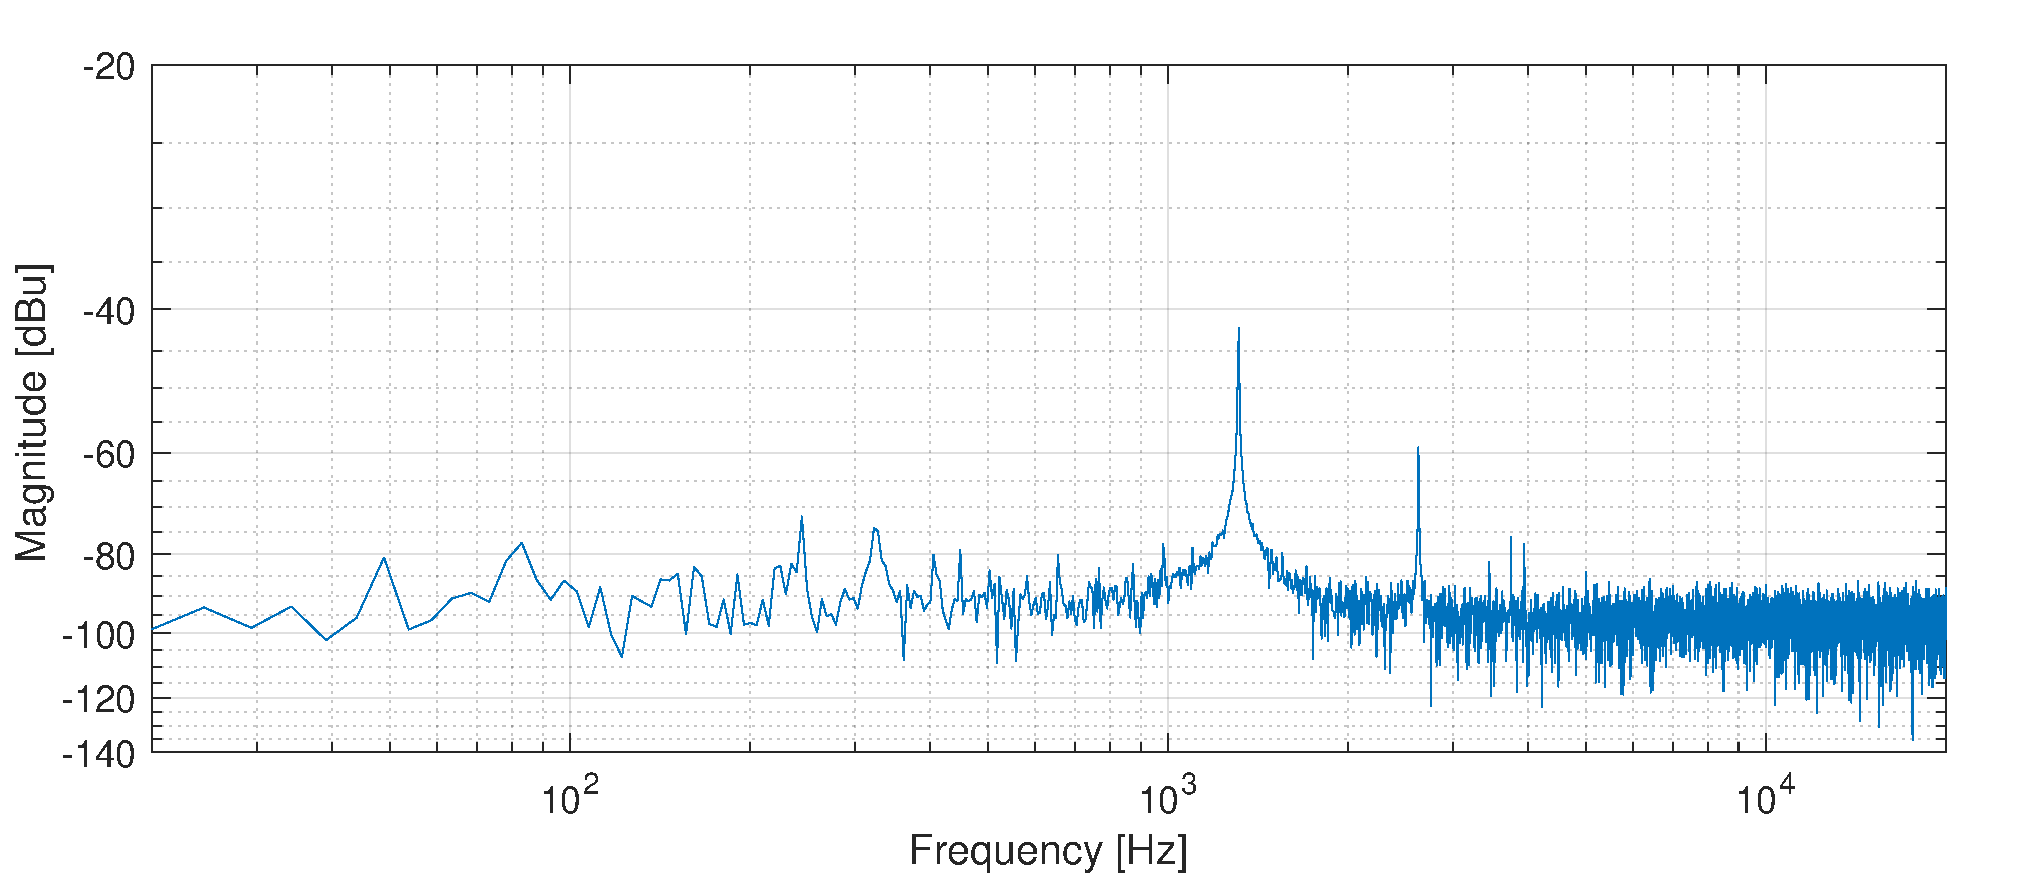
\includegraphics[width=1\textwidth]{guitar_high_E_flasholet_bridge.pdf}
		\caption{Measurement of the high E note, played as flasholet, on the bridge pickup.}
		\label{fig:appendix:high_E_bridge_flasholet}
\end{figure}

On  \autoref{fig:appendix:high_E_bridge_flasholet} it is seen that the lowest significant frequency is around \SI{1300}{\hertz} and the highest significant frequency is around \SI{2600}{\hertz}, when playing the high E note on the guitar as flasholet, using the bridge pickup. 

\chapter{Test a guitars frequency area}\label{app:frequency_area}
A test was made to get a view of the frequency area, in which the tones from a guitar lies.

\section*{Materials and setup}
To measure the frequency area on a guitar, the following materials are used:
\begin{itemize}
\item Digilent Analog Discovery 2 (Oscilloscope)
\item Fender Squier Classic Vibe Telecaster (Guitar)
\item Digilent Waveforms 2015 (PC - software)
\end{itemize}

\begin{figure}[htbp!]
\centering
\def\svgwidth{\columnwidth}
\chapter{Test a guitars frequency area}\label{app:frequency_area}
A test was made to get a view of the frequency area, in which the tones from a guitar lies.

\section*{Materials and setup}
To measure the frequency area on a guitar, the following materials are used:
\begin{itemize}
\item Digilent Analog Discovery 2 (Oscilloscope)
\item Fender Squier Classic Vibe Telecaster (Guitar)
\item Digilent Waveforms 2015 (PC - software)
\end{itemize}

\begin{figure}[htbp!]
\centering
\def\svgwidth{\columnwidth}
\input{figures/appendix/guitar_frequency_test.pdf_tex}
\caption{Setup for measuring frequency area on a guitar.}
		\label{fig:appendix:guitar_freq}
\end{figure}

\section*{Test procedure}
To the frequency area on a guitar, the following steps are made:
\begin{enumerate}
\item The materials are set up as in \autoref{fig:appendix:guitar_freq}.
\item Digilent Waveforms 2015 is set as a spectrum analyser. 
\item The guitar is set to use the neck pickup and the volume control and the tone control are turned all the way up.
\item The highest and the lowest tone on the guitar are played, measured by the oscilloscope and analysed in Digilent Waveforms 2015.
\item The guitar is set to use the bridge pickup and step 4 is repeated. 
\item The data is plotted in MATLAB.
\end{enumerate}

\section*{Results}

\begin{figure}[htbp!]
	\centering
		\includegraphics[width=1\textwidth]{guitar_low_E_neck.pdf}
		\caption{Measurement of the low E note on the neck pickup.}
		\label{fig:appendix:low_E_neck}
\end{figure}

On  \autoref{fig:appendix:low_E_neck} it is seen that the lowest significant frequency is around \SI{80}{\hertz} and the highest significant frequency is around \SI{400}{\hertz}, when playing the low E note on the guitar, using the neck pickup.

\begin{figure}[htbp!]
	\centering
		\includegraphics[width=1\textwidth]{guitar_low_E_bridge.pdf}
		\caption{Measurement of the low E note on the bridge pickup.}
		\label{fig:appendix:low_E_bridge}
\end{figure}

On  \autoref{fig:appendix:low_E_bridge} it is seen that the lowest significant frequency is around \SI{80}{\hertz} and the highest significant frequency is around \SI{730}{\hertz}, when playing the low E note on the guitar, using the bridge pickup.

\begin{figure}[htbp!]
	\centering
		\includegraphics[width=1\textwidth]{guitar_high_Cis_neck.pdf}
		\caption{Measurement of the high C\# note on the neck pickup.}
		\label{fig:appendix:high_Cis_neck}
\end{figure}

On  \autoref{fig:appendix:high_Cis_neck} it is seen that the lowest significant frequency is around \SI{1100}{\hertz} and the highest significant frequency is around \SI{4400}{\hertz}, when playing the high C\# note on the guitar, using the neck pickup.

\begin{figure}[htbp!]
	\centering
		\includegraphics[width=1\textwidth]{guitar_high_Cis_bridge.pdf}
		\caption{Measurement of the high C\# note on the bridge pickup.}
		\label{fig:appendix:high_Cis_bridge}
\end{figure}

On  \autoref{fig:appendix:high_Cis_bridge} it is seen that the lowest significant frequency is around \SI{1100}{\hertz} and the highest significant frequency is around \SI{4400}{\hertz}, when playing the high C\# note on the guitar, using the bridge pickup. 

\begin{figure}[htbp!]
	\centering
		\includegraphics[width=1\textwidth]{guitar_high_E_flasholet_bridge.pdf}
		\caption{Measurement of the high E note, played as flasholet, on the bridge pickup.}
		\label{fig:appendix:high_E_bridge_flasholet}
\end{figure}

On  \autoref{fig:appendix:high_E_bridge_flasholet} it is seen that the lowest significant frequency is around \SI{1300}{\hertz} and the highest significant frequency is around \SI{2600}{\hertz}, when playing the high E note on the guitar as flasholet, using the bridge pickup. 

\caption{Setup for measuring frequency area on a guitar.}
		\label{fig:appendix:guitar_freq}
\end{figure}

\section*{Test procedure}
To the frequency area on a guitar, the following steps are made:
\begin{enumerate}
\item The materials are set up as in \autoref{fig:appendix:guitar_freq}.
\item Digilent Waveforms 2015 is set as a spectrum analyser. 
\item The guitar is set to use the neck pickup and the volume control and the tone control are turned all the way up.
\item The highest and the lowest tone on the guitar are played, measured by the oscilloscope and analysed in Digilent Waveforms 2015.
\item The guitar is set to use the bridge pickup and step 4 is repeated. 
\item The data is plotted in MATLAB.
\end{enumerate}

\section*{Results}

\begin{figure}[htbp!]
	\centering
		\includegraphics[width=1\textwidth]{guitar_low_E_neck.pdf}
		\caption{Measurement of the low E note on the neck pickup.}
		\label{fig:appendix:low_E_neck}
\end{figure}

On  \autoref{fig:appendix:low_E_neck} it is seen that the lowest significant frequency is around \SI{80}{\hertz} and the highest significant frequency is around \SI{400}{\hertz}, when playing the low E note on the guitar, using the neck pickup.

\begin{figure}[htbp!]
	\centering
		\includegraphics[width=1\textwidth]{guitar_low_E_bridge.pdf}
		\caption{Measurement of the low E note on the bridge pickup.}
		\label{fig:appendix:low_E_bridge}
\end{figure}

On  \autoref{fig:appendix:low_E_bridge} it is seen that the lowest significant frequency is around \SI{80}{\hertz} and the highest significant frequency is around \SI{730}{\hertz}, when playing the low E note on the guitar, using the bridge pickup.

\begin{figure}[htbp!]
	\centering
		\includegraphics[width=1\textwidth]{guitar_high_Cis_neck.pdf}
		\caption{Measurement of the high C\# note on the neck pickup.}
		\label{fig:appendix:high_Cis_neck}
\end{figure}

On  \autoref{fig:appendix:high_Cis_neck} it is seen that the lowest significant frequency is around \SI{1100}{\hertz} and the highest significant frequency is around \SI{4400}{\hertz}, when playing the high C\# note on the guitar, using the neck pickup.

\begin{figure}[htbp!]
	\centering
		\includegraphics[width=1\textwidth]{guitar_high_Cis_bridge.pdf}
		\caption{Measurement of the high C\# note on the bridge pickup.}
		\label{fig:appendix:high_Cis_bridge}
\end{figure}

On  \autoref{fig:appendix:high_Cis_bridge} it is seen that the lowest significant frequency is around \SI{1100}{\hertz} and the highest significant frequency is around \SI{4400}{\hertz}, when playing the high C\# note on the guitar, using the bridge pickup. 

\begin{figure}[htbp!]
	\centering
		\includegraphics[width=1\textwidth]{guitar_high_E_flasholet_bridge.pdf}
		\caption{Measurement of the high E note, played as flasholet, on the bridge pickup.}
		\label{fig:appendix:high_E_bridge_flasholet}
\end{figure}

On  \autoref{fig:appendix:high_E_bridge_flasholet} it is seen that the lowest significant frequency is around \SI{1300}{\hertz} and the highest significant frequency is around \SI{2600}{\hertz}, when playing the high E note on the guitar as flasholet, using the bridge pickup. 

\chapter*{Test a guitars frequency area}
A test was made to get a view of the output impedance of a guitar.

\section*{Materials and setup}
To measure the output impedance on a guitar, the following materials are used:
\begin{itemize}
\item Digilent Analog Discovery 2 (Oscilloscope)
\item Fender Squier Classic Vibe Telecaster (Guitar)
\item Digilent Waveforms 2015 (PC - software)
\end{itemize}

\begin{figure}[htbp!]
\centering
\def\svgwidth{\columnwidth}
\chapter{Test a guitars frequency area}\label{app:frequency_area}
A test was made to get a view of the frequency area, in which the tones from a guitar lies.

\section*{Materials and setup}
To measure the frequency area on a guitar, the following materials are used:
\begin{itemize}
\item Digilent Analog Discovery 2 (Oscilloscope)
\item Fender Squier Classic Vibe Telecaster (Guitar)
\item Digilent Waveforms 2015 (PC - software)
\end{itemize}

\begin{figure}[htbp!]
\centering
\def\svgwidth{\columnwidth}
\input{figures/appendix/guitar_frequency_test.pdf_tex}
\caption{Setup for measuring frequency area on a guitar.}
		\label{fig:appendix:guitar_freq}
\end{figure}

\section*{Test procedure}
To the frequency area on a guitar, the following steps are made:
\begin{enumerate}
\item The materials are set up as in \autoref{fig:appendix:guitar_freq}.
\item Digilent Waveforms 2015 is set as a spectrum analyser. 
\item The guitar is set to use the neck pickup and the volume control and the tone control are turned all the way up.
\item The highest and the lowest tone on the guitar are played, measured by the oscilloscope and analysed in Digilent Waveforms 2015.
\item The guitar is set to use the bridge pickup and step 4 is repeated. 
\item The data is plotted in MATLAB.
\end{enumerate}

\section*{Results}

\begin{figure}[htbp!]
	\centering
		\includegraphics[width=1\textwidth]{guitar_low_E_neck.pdf}
		\caption{Measurement of the low E note on the neck pickup.}
		\label{fig:appendix:low_E_neck}
\end{figure}

On  \autoref{fig:appendix:low_E_neck} it is seen that the lowest significant frequency is around \SI{80}{\hertz} and the highest significant frequency is around \SI{400}{\hertz}, when playing the low E note on the guitar, using the neck pickup.

\begin{figure}[htbp!]
	\centering
		\includegraphics[width=1\textwidth]{guitar_low_E_bridge.pdf}
		\caption{Measurement of the low E note on the bridge pickup.}
		\label{fig:appendix:low_E_bridge}
\end{figure}

On  \autoref{fig:appendix:low_E_bridge} it is seen that the lowest significant frequency is around \SI{80}{\hertz} and the highest significant frequency is around \SI{730}{\hertz}, when playing the low E note on the guitar, using the bridge pickup.

\begin{figure}[htbp!]
	\centering
		\includegraphics[width=1\textwidth]{guitar_high_Cis_neck.pdf}
		\caption{Measurement of the high C\# note on the neck pickup.}
		\label{fig:appendix:high_Cis_neck}
\end{figure}

On  \autoref{fig:appendix:high_Cis_neck} it is seen that the lowest significant frequency is around \SI{1100}{\hertz} and the highest significant frequency is around \SI{4400}{\hertz}, when playing the high C\# note on the guitar, using the neck pickup.

\begin{figure}[htbp!]
	\centering
		\includegraphics[width=1\textwidth]{guitar_high_Cis_bridge.pdf}
		\caption{Measurement of the high C\# note on the bridge pickup.}
		\label{fig:appendix:high_Cis_bridge}
\end{figure}

On  \autoref{fig:appendix:high_Cis_bridge} it is seen that the lowest significant frequency is around \SI{1100}{\hertz} and the highest significant frequency is around \SI{4400}{\hertz}, when playing the high C\# note on the guitar, using the bridge pickup. 

\begin{figure}[htbp!]
	\centering
		\includegraphics[width=1\textwidth]{guitar_high_E_flasholet_bridge.pdf}
		\caption{Measurement of the high E note, played as flasholet, on the bridge pickup.}
		\label{fig:appendix:high_E_bridge_flasholet}
\end{figure}

On  \autoref{fig:appendix:high_E_bridge_flasholet} it is seen that the lowest significant frequency is around \SI{1300}{\hertz} and the highest significant frequency is around \SI{2600}{\hertz}, when playing the high E note on the guitar as flasholet, using the bridge pickup. 

\caption{Setup for measuring frequency area on a guitar.}
		\label{fig:appendix:guitar_freq}
\end{figure}

\section*{Test procedure}


\begin{enumerate}
\item The materials are set up as in \autoref{fig:appendix:guitar_output_impedance}.
\item 
\item  
\item  
\item 
\item 
\end{enumerate}

\section*{Results}

\begin{figure}[htbp!]
	\centering
		\includegraphics[width=1\textwidth]{guitar_low_E_neck.pdf}
		\caption{Measurement of the low E note on the neck pickup.}
		\label{fig:appendix:low_E_neck}
\end{figure}

On  \autoref{fig:appendix:low_E_neck} it is seen that the lowest significant frequency is around \SI{80}{\hertz} and the highest significant frequency is around \SI{400}{\hertz}, when playing the low E note on the guitar, using the neck pickup.


\chapter{Reverb and Delay Simulation and Test}\label{app:reverb}

The MATLAB simulation code for delay effect. 
\includeCode{delay.m}{matlab}{1}{39}{The delay simulation matlab code}{code:delay_sim}{code/design/}

The MATLAB simulation code for \gls{reverb} effect. 
\includeCode{reverb.m}{matlab}{1}{80}{The reverb simulation matlab code}{code:reverb_sim}{code/design/}


\chapter{Flanger and Chorus MATLAB code and simulation}x

The Matlab code for the flanger effect is:

\begin{lstlisting}[language=Matlab, caption= Matlab code for flanger effect]

%Flanger Effect
%Group 641
%Mohamed Gabr, Jonas and Sebastian


filename = 'inputttt.wav'; 
%The filename is inserted here, should be in the same directory as the
%codefile.
[input, fs] = audioread(filename, 'native');
%input samples and sample rate are extracted from the file.
input = input / (max(abs(input)));
%the input is rescaled in order to have values between -1 and 1. 
fl = 100;  
%LFO Frequency is chosen here.
sample_no = length(input); 
%Length of the input samples table.
g = 100; 
%Gain
delay_s = 0.0050; 
% The maximum delay in seconds.
after_delay = (1:1:sample_no); 
before_delay = (1:1:sample_no);
output = (1:1:sample_no);
%Needed tables in the code are intialized to make the code faster.
disp('max delay')
max_delay = delay_s * fs  
%Convert the maximum delay from delay in seconds to delay in samples.

buffer = zeros(1,abs(round(max_delay))); 
%intializing the buffer array.

for i = 1:1:sample_no  %Loop that treats a sample per iteration. 
 delay = max_delay * cos(2*pi*i*(fl/fs)); %Calculate time varying delay 
 %(unit is samples)
 buffer = [buffer(2:end) input(i)]; 
 %move the values in the buffer ==> first value overwritten, one new 
 %value added at the end.
 if abs(delay) < 1   %All delay values less than zero are considered as
  %not having a delay
  after_delay(i) = 0;
 else
  if floor(delay) == delay || abs(floor(delay)) >= floor(max_delay)
   after_delay(i) = buffer(round(abs(delay))) * g;
   %Treating the case when the delay is an integer and when it has a
   %value bigger than the maximum delay. 
  else %Treating the case when the delay is not an integer
   x1 = abs(floor(delay));
   x2 = x1 + 1;
   y1 = buffer(x1);
   y2 = buffer(x2);
   coeff = (y1 - y2)/(x1 - x2);
   %Making a linear approximation between the samples to increase
   %precision
   after_delay(i) = delay * coeff * g;  %sound from the delay line
   %in the block diagram 
  end
 end
 before_delay(i) = input(i);  %sound from the direct line
 output(i) = after_delay(i) + before_delay(i); %output delayed signal 
end
output = output / max(abs(output)); %output is rescaled to values between
% -1 and 1 to avoid clipping. 
audiowrite('out_flan.wav',output,fs); %Writing the values in a file, 
% PS: audiowrite will clip if the values are not between -1 and 1. 
plot(output,'r') %plotting the output samples in red.
hold on
grid
plot(before_delay,'b') %plotting the input samples in blue on the same fig.




\end{lstlisting}


The code is commented for the user's instruction.\\

The Matlab code for the chorus effect is:

\begin{lstlisting}[language=Matlab, caption= Matlab code for chorus effect]

%Chorus Effect
%Group 641
%Mohamed, Jonas and Sebastian

filename = 'inputttt.wav'; %Typing the filename, should be in same 
%directory as the codefile
[input, fs] = audioread(filename);
%input samples and sample rate are extracted from the file.
input = input / (max(abs(input)));
%the input is rescaled in order to have values between -1 and 1.
lines = 5; %number of chorus lines 
fl = randi(10,1,lines);
%LFO Frequencies for each line are generated.
delay = (1:1:lines);
%Delay table generated here to speed the coding. 
sample_no = length(input); 
%Length of the input samples
g = rand(1,lines); 
%Gain values generated here
delay_s = 0.025; 
% Maximum delay in seconds 
after_delay = rand(lines, sample_no); 
before_delay = (1:1:sample_no);
output = (1:1:sample_no);
% Generating tables to speed the code. 
max_delay = delay_s * fs  
%convert the delay from delay in seconds to delay in samples. 


buffer = zeros(1,abs(round(max_delay))); %create the buffer array 

for i = 1:1:sample_no %loop that gives one output sample per iteration
 buffer = [buffer(2:end) input(i)]; %moving buffer values
 before_delay(i) = input(i); %Value before delay
 output(i) = before_delay(i); %adding it to one output sample
 for j = 1:1:lines %Generating delays and then samples after delay for 
 %each chorus line
   delay(j) = max_delay * cos(2*pi*i*(fl(j)/fs)); %Calculate time  
   %varying delay (unit is samples)
   if abs(delay(j)) < 1 %Treating the case where the delay is less 
   %than one.
	 after_delay(j,i) =0;
   else
	 if floor(delay(j)) == delay(j) || abs(floor(delay(j))) >= floor(max_delay)
	   after_delay(j,i) = buffer(round(abs(delay(j)))) * g(j);
	   %Treating the case when the delay is an integer and when it has a
	   %value bigger than the maximum delay. 
	 else  %Treating the case when the delay is not an integer
	   x1 = abs(floor(delay(j)));
	   x2 = x1 + 1;
	   y1 = buffer(x1);
	   y2 = buffer(x2);
	   coeff = (y1 - y2)/(x1 - x2);
	   %Making a linear approximation between the samples to increase
	   %precision
	   after_delay(j,i) = delay(j) * coeff * g(j);  
	   %sound from the delay line in the block diagram
	 end
   end
   output(i) = output(i) + after_delay(j,i);
   %Signal output sample
 end
end
output = output / max(abs(output)); %output is rescaled to values between
% -1 and 1 to avoid clipping. 
audiowrite('out_chor.wav',output,fs); %Writing the values in a file, 
% PS: audiowrite will clip if the values are not between -1 and 1.
plot(output,'r') %plotting the output samples in red.
hold on
grid
plot(before_delay,'b') %plotting the input samples in blue on the same fig.



\end{lstlisting}

The codes where simulated on different audiofiles. 
\chapter{Test of Signal to Noise Ratio}\label{app:test:snr}

The test of SNR of the guitar is going to be presented in this appendix. It will include the used material and setup, the test procedure and the results. \\

\section{Material and Setup}

In order to perform this test, the following material has been used:

\begin{itemize}
	\item Electric guitar used during the project (same for all tests)
	\item Analog Discovery Digilent 2 USB Oscilloscope
	\item A computer with Waveforms 2015 and MATLAB
	\item Wires
\end{itemize}


The first step is to connect the oscilloscope to the computer with a USB cable and then connect the oscilloscope to the guitar. Different converters maybe needed. The user should ensure that none of the connections are loose in order to obtain the best results possible. \\

\section{Test Procedure}

The test is done in two steps. First, noise is measured without the guitar connected. It is done by measuring the maximum and the minimum amplitude of the signal of the ocilloscope alone. \\

The second test to make is to measure the noise with the guitar connected by taking the maximum and the minimum amplitude of the signal with the guitar connected.  \\

For each of the tests, a difference between the maximum and the minimum is made. The wanted value is the difference between the two resulting calculations. \\

\section{Results}

The plot of the signal amplitude without the guitar is shown in figure \ref{fig:without_guitar}. \\

\begin{figure}[hbt]
  \centering
  \includegraphics[width=1\textwidth]{without_guitar.pdf}
  \caption{Signal Amplitude without the guitar connected}
  \label{fig:without_guitar}
\end{figure}

The maximum value obtained is -0.002355 V and the minimum is -0.0034 V which gives a difference of 0.001045 V. \\

The plot of the signal amplitude with the guitar is shown in figure \ref{fig:with_guitar}. \\

\begin{figure}[hbt]
  \centering
  \includegraphics[width=1\textwidth]{with_guitar.pdf}
  \caption{Signal Amplitude without the guitar connected}
  \label{fig:with_guitar}
\end{figure}

The maximum and the minimum obtained from the aquired data seems to be -0.003693 V and -0.00202 V respectively which gives a difference of 0.001673 V.  \\
The difference between the two (max-min) is then 0.000628 V. \\
Supposing that the maximum signal that can be obtained peak to peak from the guitar is 2 V according to the test in \autoref{app:guitar_max_amplitude}, the signal to noise ratio is then:

\begin{equation}
	SNR = 20 \cdot log_{10}(\frac{2}{0.000628} = 70.06dB
	\end{equation}

Where:

$SNR$ is the signal to noise ratio of the guitar in dB \\


This result is subject to many errors. From the graphs in the two cases, it can be seen that the oscilloscope precision is not enough to get a clear conclusion. The sure conclusion is that the noise is of the order of 0.0001V but the exact value cannot be verified. In all cases, an SNR of the order 70dB can be assumed sufficient.
\chapter{Test of preamp frequency response}\label{app:preamp_frequency_response}
A test was made to get a view of the frequency response of the preamp.

\section*{Materials and setup}
To measure the frequency response of the preamp, the following materials are used:
\begin{itemize}
\item Digilent Analog Discovery 2 (Oscilloscope)
\item Digilent Waveforms 2015 (PC - software)
\end{itemize}


\begin{figure}[htbp!]
\centering
\begin{picture}(0,0)%
\includegraphics{guitar_output_phase_impedance.pdf}%
\end{picture}%
\setlength{\unitlength}{4144sp}%
%
\begingroup\makeatletter\ifx\SetFigFont\undefined%
\gdef\SetFigFont#1#2#3#4#5{%
  \reset@font\fontsize{#1}{#2pt}%
  \fontfamily{#3}\fontseries{#4}\fontshape{#5}%
  \selectfont}%
\fi\endgroup%
\begin{picture}(4205,1464)(4129,-2773)
\put(7426,-1996){Osc}%
\put(6346,-1996){Osc}%
\put(6346,-2176){Ch2}%
\put(7966,-1996){Osc}%
\put(8011,-2176){W1}%
\put(4681,-2086){DSP}%
\put(6346,-1771){+}%
\put(6346,-2401){-}%
\put(7426,-1771){+}%
\put(7471,-2401){-}%
\put(6796,-1591){Preamp}%
\put(7426,-2176){ch1}%
\end{picture}%
\caption{Setup for measuring phase of output impedance on a guitar.}
		\label{fig:appendix:preamp_frequency_response}
\end{figure}


\section*{Test procedure}
\begin{enumerate}
\item The materials are set up as in \autoref{fig:appendix:preamp_frequency_response}.
\item The Digilent Waveform 2015 is set as a Network analyser.
\item  The \gls{preamp} is set to have an gain of \SI{0}{\decibel}
\item  The network analyser is set to measure $dB$ from \SI{20}{\hertz} to \SI{20}{\kilo\hertz} with 10000 sample.
\item The measured data on the Osc ch1 and ch2 is used in the following formula $\text{dB diffetent}= \text{ch2}-\text{ch1}$ which depend on the frequency. 
\item The data is plotted in MATLAB.
\end{enumerate}

\section*{Results}

\begin{figure}[htbp!]
	\centering
		\includegraphics[width=1\textwidth]{preamp_frequency_responce.pdf}
		\caption{Measurement of the real output impedance of the three pickup settings.}
		\label{fig:appendix:preamp_amplitude}
		\includegraphics[width=1\textwidth]{preamp_frequency_responce_phase.pdf}
		\caption{Measurement of the imaginary output impedance of the three pickup settings.}
		\label{fig:appendix:preamp_phase}
\end{figure}

\chapter{Test of effect run time}\label{app:effect_run_time}

The tests of the time needed to run effects are presented in this appendix.

\section*{Materials and setup}
To measure the time consumption of each effect, the following materials are used:
\begin{itemize}
\item Digilent Analog Discovery 2 (Oscilloscope)
\item Digilent Waveforms 2015 (PC - software)
\item Ezdsp board
\end{itemize}


\begin{figure}[htbp!]
	\centering
		\includegraphics[width=0.5\textwidth]{run_time.pdf}
		\caption{Illustration showing the location of the measurement point on the EZdsp}
		\label{fig:run_time_test_point}
\end{figure}

\includeCode{mainas.asm}{assembly}{12}{21}{Example of runtime testing main program}{code:mainas_asm}{code/design/}

\section*{Test procedure}
\begin{enumerate}
\item The materials are set up as in \autoref{fig:run_time_test_point}.
\item The Digilent Waveform 2015 is set as a Scope.
\item  The XF led bit is set at the beginning of the program and cleared in the end of the program, in the mainas file, see example \autoref{code:mainas_asm}. The time from when the LED is being illuminated until it is turned off is the runtime, also measured using the magnitude as shown in \autoref{fig:run_time_test_point}. 
\item  The Scope is then used to measure the XF LED runtime 
\item The data is plotted in MATLAB.
\end{enumerate}

\section*{Reverb run time}
The following \autoref{fig:reverb_time_test} shows the measurement results of the \gls{reverb} assembly program runtime.
\begin{figure}[htbp!]
	\centering
		\includegraphics[width=1\textwidth]{reverb_run_time.pdf}
		\caption{The figure shows the runtime of the \gls{reverb} assembly program}
		\label{fig:reverb_time_test}
\end{figure}

According to \autoref{fig:reverb_time_test}, the \gls{reverb} runtime is \SI{2.25}{\micro\second}

\section*{Cordic run time}
The following \autoref{fig:cordic_time_test} shows the measurement results of the cordic assembly program runtime.
\begin{figure}[htbp!]
	\centering
		\includegraphics[width=1\textwidth]{cordic_run_time.pdf}
		\caption{The figure shows the runtime of the cordic assembly program}
		\label{fig:cordic_time_test}
\end{figure}

According to \autoref{fig:cordic_time_test}, the cordic runtime is \SI{1.3}{\micro\second}

\section*{Flanger run time}
The following \autoref{fig:flanger_time_test} shows the measurement results of the flanger assembly program runtime.
\begin{figure}[htbp!]
	\centering
		\includegraphics[width=1\textwidth]{flanger_run_time.pdf}
		\caption{The figure shows the runtime of the flanger assembly program}
		\label{fig:flanger_time_test}
\end{figure}

According to \autoref{fig:flanger_time_test}, the flanger run time is \SI{2.4}{\micro\second}
\chapter{Test of input and output impedance of the TS464 operational amplifier}
\label{app:opamp_impedance}

The test was made to measure the input- and output- impedance of the TS464 \gls{opamp}. \\

\section{Material and Setup}

In order to perform this test, the following material has been used:

\begin{itemize}
	\item TS464 operational amplifier
	\item Analog Discovery Digilent 2 USB Oscilloscope
	\item A computer with Waveforms 2015 and MATLAB
	\item Wires
\end{itemize}


At first the input impedance will be measured, using the setup in \autoref{fig:opamp_zi}, where $R_S$ is chosen \SI{1}{\mega\ohm}. Afterwords the output impedance will be measured, using the setup in \autoref{fig:opamp_zo}, where $R$ is set to \SI{1}{\kilo\ohm}. In both cases $V_S$ is set to make a \SI{1}{\kilo\hertz} sine, with an amplitude of \SI{0.5}{\volt} and a \SI{2}{\volt} offset.

\begin{figure}[h!]
\centering
\begin{circuitikz}\draw (0,0)
(3,.5) node[op amp]{}
(-1,0)to[R=$R_S$] (1,0)
(1,0)to[short]  (2,0)
(4,.5)to[short] (5,.5)
to[short] (5,2)
to[short] (1,2)
to[short] (1,1)
to[short] (2,1)
(-1,0)to[short](-1.5,0)
to[sV=$V_S$] (-1.5,-2)
node[ground]{}
(1,0)to[sV=$V_2$] (1,-2)
node[ground]{}
(5,.5)to[R=$R_L$] (5,-2)
node[ground]{}

;\end{circuitikz}
\caption{Test setup for measuring input impedance of an \gls{opamp}, where $R_S =$\SI{1}{\mega\ohm} and $R_L = $\SI{1}{\kilo\ohm}.}
\label{fig:opamp_zi}
\end{figure}

\begin{figure}[h!]
\centering
\begin{circuitikz}\draw (0,0)
(3,.5) node[op amp]{}
(-1,0)to[R=$R_S$] (1,0)
(1,0)to[short]  (2,0)
(4,.5)to[short] (5,.5)
to[short] (5,2)
to[short] (1,2)
to[short] (1,1)
to[short] (2,1)
(-1,0)to[short](-1.5,0)
to[short] (-1.5,-2)
node[ground]{}
(5,.5)to[R=$R_L$] (7.5,.5)
to[sV=$V_S$] (7.5,-2)
node[ground]{}
(5,.5)to[sV=$V_2$] (5,-2)
node[ground]{}

;\end{circuitikz}
\caption{Test setup for measuring output impedance of an \gls{opamp}, where $R_S = R_L = $\SI{1}{\kilo\ohm}.}
\label{fig:opamp_zo}
\end{figure}



\section{Test Procedure}

For the input impedance the steps are as follows:
\begin{itemize}
\item Measure the amplitude of the signal at $V_S$.
\item Measure the amplitude of the signal at $V_2$ 
\item Subtract $V_2$ from $V_S$ to get the amplitude of $V_1$. 
\item Use \autoref{eq:opamp_zi} to calculate the input impedance.
\end{itemize}

\begin{equation}\label{eq:opamp_zi}
        Z_i = \frac{V_2}{V_1} \cdot R_S
        \addunit{\si{\ohm}}
    \end{equation}

    \startexplain
        \explain{$Z_i$ is the input impedance of the \gls{opamp}}{\si{\ohm}}
        \explain{$V_2$ is the voltage over the input of the \gls{opamp}}{\si{\volt}}
        \explain{$V_1$ is the voltage $R_S$}{\si{\volt}}
    \stopexplain
    
For the output impedance the steps are as follows:
\begin{itemize}
\item Measure the amplitude of the signal at $V_S$.
\item Measure the amplitude of the signal at $V_2$ 
\item Subtract $V_2$ from $V_S$ to get the amplitude of $V_1$. 
\item Use \autoref{eq:opamp_zo} to calculate the input impedance.
\end{itemize}

\begin{equation}\label{eq:opamp_zo}
        Z_o = \frac{V_2}{V_1} \cdot R
        \addunit{\si{\ohm}}
    \end{equation}

    \startexplain
        \explain{$Z_o$ is the output impedance of the \gls{opamp}}{\si{\ohm}}
        \explain{$V_2$ is the voltage over the output of the \gls{opamp}}{\si{\volt}}
        \explain{$V_1$ is the voltage $R$}{\si{\volt}}
    \stopexplain

\section{Results}

In \ref{fig:opamp_zi_v0} the measurement of $V_S$, when measuring the input impedance shown, and in \ref{fig:opamp_zi_v2} the measurement of $V_2$, when measuring the input impedance shown. \\

\begin{figure}[hbt]
  \centering
  \includegraphics[width=1\textwidth]{opamp_zi_v0}
  \caption{Measurement of $V_S$, when measuring the input impedance.}
  \label{fig:opamp_zi_v0}
\end{figure}

\begin{figure}[hbt]
  \centering
  \includegraphics[width=1\textwidth]{opamp_zi_v2}
  \caption{Measurement of $V_2$, when measuring the input impedance.}
  \label{fig:opamp_zi_v2}
\end{figure}

In \ref{fig:opamp_zo_v0} the measurement of $V_S$, when measuring the output impedance shown, and in \ref{fig:opamp_zo_v2} the measurement of $V_2$, when measuring the output impedance shown. \\

\begin{figure}[hbt]
  \centering
  \includegraphics[width=1\textwidth]{opamp_zo_v0}
  \caption{Measurement of $V_S$, when measuring the output impedance.}
  \label{fig:opamp_zo_v0}
\end{figure}

\begin{figure}[hbt]
  \centering
  \includegraphics[width=1\textwidth]{opamp_zo_v2}
  \caption{Measurement of $V_2$, when measuring the output impedance.}
  \label{fig:opamp_zo_v2}
\end{figure}

The amplitudes of $V_S$ and $V_2$, when measuring the input impedance are measured to \SI{489}{\milli\volt} and \SI{441}{\milli\volt}. $V_1$ here by is calculated to \SI{48}{\milli\volt}. The input impedance of the \gls{opamp} is therefore as in \autoref{}.

\begin{equation}\label{eq:opamp_zi}
        Z_i = \frac{441}{48} \cdot 10^6 = 9.18
        \addunit{\si{\mega\ohm}}
    \end{equation} 
    
The amplitudes of $V_S$ and $V_2$, when measuring the output impedance are measured to \SI{493}{\milli\volt} and \SI{444}{\milli\volt}. $V_1$ here by is calculated to \SI{49}{\milli\volt}. The input impedance of the \gls{opamp} is therefore as in \autoref{}.

\begin{equation}\label{eq:opamp_zo}
        Z_o = \frac{444}{49} \cdot 10^3 = 9.06
        \addunit{\si{\kilo\ohm}}
    \end{equation} 
\chapter{Test of cordic shape and offset}\label{app:cordic_shape}
A test was made to get a view of the cordic shape and offset.

\section*{Materials and setup}
To measure the cordic shape and offset, the following materials are used:
\begin{itemize}
\item Digilent Analog Discovery 2 (Oscilloscope)
\item Digilent Waveforms 2015 (PC - software)
\end{itemize}

\begin{figure}[htbp!]
	\centering
		\includegraphics[width=1\textwidth]{cordic_435mHz.pdf}
		\caption{hgfs}
		\label{fig:appendix:cordic_435mHz}
\end{figure} % Include chapters

% For use if report is split up in parts
\bookmarksetup{startatroot}% Goto root of Table of Contents
\addtocontents{toc}{\bigskip}% Add space before next item in Table of Contents

% Appearance of the bibliography
\iflanguage{english}{%
\bibliographystyle{setup/plainnat_en}%
}{%
\bibliographystyle{setup/plainnat_dk}%
}



\bibliography{bib/conference,bib/datasheets,bib/mastersthesis,bib/newsarticles,bib/phdthesis,bib/sciencearticles,bib/standards,bib/techreports,bib/websites,bib/books}
\label{bib:mybiblio}



%\setlength{\chapnumb}{2cm} % Ændrer længden på stregen under kapiteloverskriften så den passer til bilag
\appendix % Start of appendix
\addtocontents{toc}{\protect\setcounter{tocdepth}{0}} 
%\input{chapters/appendices/_appendices} % Include appendices

\end{document}
